\documentclass[12pt]{article}
\usepackage{lmodern}
\usepackage{amsmath}
\usepackage{amssymb}
\usepackage{graphicx}
\usepackage{caption}
\captionsetup{font=small, labelfont=bf}
\renewcommand{\arraystretch}{1.1}
\usepackage{float}
\usepackage[round]{natbib}
\setcitestyle{round}
\usepackage{hyperref}
\usepackage{geometry}
\usepackage{setspace}
\usepackage{booktabs}
\usepackage{array}
\usepackage{subcaption}
\usepackage{xcolor}
\usepackage{colortbl}
\usepackage{fancyhdr}

% Set reasonable margins for a professional report
\geometry{margin=1in}

% Configure running headers
\pagestyle{fancy}
\fancyhf{}
\fancyhead[L]{\textcolor{gray}{\nouppercase{\leftmark}}}
\fancyhead[R]{\textcolor{gray}{\thepage}}
\renewcommand{\headrulewidth}{0pt}

% Configure hyperlinks
\hypersetup{
    colorlinks=true,
    linkcolor=black,
    urlcolor=black,
    citecolor=black
}

% Title page information
\title{Customer Churn in Banking: An Integrated Approach Combining Survival Analysis and Machine Learning}
\author{Andrew Sullivan}
\date{October~23,~2025}

\begin{document}

% Title page
\begin{titlepage}
  \centering
  \vspace*{2cm}
  \Huge\textbf{Customer Churn in Banking:}\\An Integrated Approach Combining\\Survival Analysis and Machine Learning
  \vspace{1.5cm}

  \large
  Andrew Sullivan\\[0.5cm]
  Independent Research Project\\[0.5cm]
  Fall~2025
  
  \vfill
\end{titlepage}
\thispagestyle{plain}

\newpage
\thispagestyle{plain}
\begin{abstract}
Customer retention has emerged as a strategic priority for banks amid intensifying competition, shrinking margins, and rising digital expectations. Using 10,000 retail-banking records, this study integrates exploratory analysis, survival modeling, and machine learning to explain and predict churn. Building on prior survival-analysis work, this study quantifies risk factors, estimates time to churn, and delivers a Random Forest classifier with 85.9\% accuracy for proactive risk scoring. Inactivity, product-portfolio imbalance, and lifecycle stage dominate risk; inactive members face 1.88× higher churn. Combining Kaplan–Meier and Cox models with interpretable ensemble methods provides both temporal and probabilistic insights, enabling targeted re-engagement campaigns, lifecycle retention programs, and portfolio optimization.
\end{abstract}

\newpage
\pagenumbering{roman}
\pagestyle{plain}
\tableofcontents
\newpage
\pagenumbering{arabic}
\pagestyle{fancy}

\section{Introduction}
\markboth{INTRODUCTION}{}
Customer churn, the process by which customers close accounts or cease doing business with a firm, is a critical concern for banks. On average, acquiring a new customer can cost five to seven times more than retaining an existing one \citep{businessbuilders2024cost}, and even modest improvements in retention can yield disproportionate profit increases \citep{kumar2022customerretention}. For many financial institutions, high churn rates translate into substantial losses in lifetime value. Effective churn management therefore requires not only understanding who leaves and when, but also why they leave and how the bank can intervene.

Using a rich dataset of ten thousand customers made publicly available by \citet{kollipara2022bank}, this study investigates demographic, behavioral and financial attributes to determine how they contribute to attrition. The analysis employs survival analysis and machine learning techniques to estimate individual churn probabilities and design targeted retention programs. Specifically, this study conducts exploratory data analysis to identify predictive factors, quantifies time‑to‑churn patterns using Kaplan–Meier estimators and Cox proportional hazards models, builds a random forest classifier for proactive risk scoring, validates model performance against alternative algorithms, and translates statistical findings into actionable business recommendations with quantified ROI. The methods and insights presented here demonstrate an integrated approach to analytics‑driven customer retention applicable to similar banking contexts.

\subsection{Literature Review}
Customer retention has emerged as a fundamental business imperative across service industries, driven by the well-established principle that retaining existing customers costs significantly less than acquiring new ones \citep{businessbuilders2024cost}. In banking, this dynamic is particularly pronounced, with customer lifetime values ranging from \$2,000 to \$4,000 for typical retail banking relationships \citep{meleis2010clv}.

Early approaches to churn management relied on customer relationship management (CRM) systems that operated reactively, identifying problems only after customers had begun to disengage \citep{singh2024productchurn}. The shift toward proactive churn prediction leverages machine learning techniques to identify customers at risk based on demographic, behavioral, and transactional patterns observed before explicit signals of dissatisfaction emerge. \citet{singh2024productchurn} conducted a comprehensive comparative analysis of multiple ML algorithms on the same dataset used in this study, achieving optimal performance with Random Forest (78.3\% accuracy, 69.3\% sensitivity using SMOTE oversampling) and XGBoost (83.9\% accuracy, 60.1\% sensitivity). Their findings validated several critical patterns in bank customer behavior, including elevated churn rates among German customers and the optimal retention profile for customers holding exactly two products, patterns that receive independent confirmation in our exploratory analysis.

However, traditional classification approaches, while effective at answering \emph{who} will churn, provide limited insight into \emph{when} churn occurs or how temporal factors contribute to attrition risk. Survival analysis methods, adapted from biostatistics and telecommunications churn studies \citep{desai_customer_survival}, offer a complementary framework for modeling time-to-event outcomes. Model interpretability has also emerged as a critical requirement for operational deployment, with recent work demonstrating the utility of SHAP (Shapley Additive Explanations) frameworks for explaining black-box predictions in banking contexts \citep{peng2023interpretability}. The translation of predictive insights into actionable business strategy also remains a critical gap in academic churn research \citep{brito2024framework}.

This study bridges these gaps by combining survival analysis methodology with comparative ML evaluation and strategic business planning. The analysis extends the findings of \citet{singh2024productchurn} through several methodological contributions: (1) incorporation of Kaplan–Meier survival curves and Cox proportional hazards modeling to quantify temporal churn patterns; (2) systematic comparison of SMOTE oversampling versus class-weight balancing strategies; (3) application of SHAP values and partial dependence plots for granular model interpretability; and (4) translation of statistical findings into quantified ROI projections and phased implementation strategies.

\section{Methods}
\markboth{METHODS}{}
This section describes the data sources, preprocessing procedures, statistical methods, and model development approaches employed in the analysis. The methodology encompasses three main components: exploratory data analysis to identify patterns and guide feature selection, survival analysis to quantify temporal churn patterns, and predictive modeling to develop actionable risk scoring tools.

\subsection{Dataset and Pre‑Processing}
\subsubsection{Data Source and Structure}
The analysis uses the \emph{Bank Customer Churn} dataset compiled by \citet{kollipara2022bank}.  The dataset comprises 10,000 anonymised records of retail banking customers.  Each record includes demographic variables (e.g.\ gender, geography, age), behavioral indicators (active membership status, tenure), product usage metrics (number of products, credit card ownership), financial variables (balance, estimated salary, credit score) and experiential measures (satisfaction score, complaint status, card type and loyalty points).  In addition to the feature columns, the dataset includes a binary target variable indicating whether the customer exited the bank.  The data card provided by the dataset author notes that identifier columns such as RowNumber and CustomerId have no predictive value and should be dropped.

\subsubsection{Cleaning and Feature Engineering}
Records with missing or duplicate values were removed. Identifier fields (RowNumber, CustomerId) were discarded. An age\_group feature was engineered by discretising the Age variable into six categories (18–30, 31–40, 41–50, 51–60, 61–70, 70+) to capture non‑linear lifecycle effects while preserving interpretability. One‑hot encoding was applied to categorical variables (gender and geography). The complaint indicator was intentionally excluded from predictive models as a lagging indicator of churn. Continuous variables were standardized using Z-score normalization primarily for Cox regression compatibility; tree-based algorithms are invariant to scaling but standardization was applied consistently across all models.

\subsubsection{Feature Selection and Rationale}
Linear correlation analysis with churn was used to identify predictive features. Features with moderate to strong correlations (|r| $\geq$ 0.10) were retained as core predictors, while those with minimal linear relationships (|r| $<$ 0.10) were excluded from modeling. The threshold of |r| $\geq$ 0.10 represents a standard heuristic for identifying meaningful associations in behavioral data; correlations below this threshold typically indicate negligible linear relationships that are unlikely to meaningfully contribute to prediction models. The complaint indicator was intentionally excluded because it represents a lagging indicator of churn that would create a methodological degenerate case \citep{kumar2022customerretention}. This selective approach balances predictive power with interpretability, emphasizing modifiable factors (number of products, activity status) and strong demographic predictors (age, geography) that directly inform intervention strategies. Features with weak linear correlation but anticipated non-linear effects were retained for tree-based algorithms capable of capturing complex patterns.


\subsection{Survival Analysis}
Survival analysis models the time until an event occurs and is well suited for churn studies where the timing of attrition matters. The fundamental quantity is the survival function \(S(t) = \Pr(T > t)\), which represents the probability of surviving at least to time \(t\). The hazard function \(h(t)\) quantifies the instantaneous risk of experiencing the event at time \(t\), given survival until \(t\).

\subsubsection{Kaplan–Meier Estimator}
Kaplan–Meier (K–M) estimators, first described by \citet{dudley2016kaplan}, are non‑parametric methods that estimate the survival function based solely on observed event times and censoring. K–M curves were computed for customer segments stratified by age group, number of products, activity status, geography, gender, and balance group. Log-rank tests were performed to assess statistical significance of differences between groups, testing the null hypothesis that survival distributions are identical across strata.

\subsubsection{Cox Proportional Hazards Model}
The Cox proportional‑hazards model is a multivariable regression that relates the hazard of the event to multiple covariates simultaneously \citep{sthda_cox}. The hazard function in the Cox model is specified as
\[ h(t) = h_0(t) \exp(\beta_1 x_1 + \beta_2 x_2 + \cdots + \beta_p x_p), \]
where \(h_0(t)\) is the baseline hazard and the coefficients \(\beta_i\) quantify the effect of covariate \(x_i\) on the hazard. Hazard ratios (\(\exp(\beta_i)\)) greater than one indicate increased risk, while ratios below one signify protective effects.

A Cox model was fitted excluding the complaint variable to avoid its dominance. Covariates included gender, tenure, balance, number of products, activity status, geography, and age group dummy variables. Model fit was assessed using the concordance index (C-index), which measures the proportion of comparable pairs where the predicted outcomes are correctly ordered. The proportional hazards assumption was tested using Schoenfeld residuals; all covariates satisfied the assumption (no significant time-dependency), validating the hazard ratio interpretations.

\subsection{Predictive Modeling}
A random forest classifier was trained on the curated feature set to identify at‑risk customers before a complaint is lodged. Random forests are ensemble learning techniques that combine the output of many decision trees built on bootstrap samples of the data \citep{geeksforgeeks_randomforest}. Each tree considers a random subset of features at each split and contributes a vote to the final prediction. Formally, for a random forest with \(B\) trees, the ensemble prediction is
\[ \hat{f}_{\text{RF}}(\mathbf{x}) = \frac{1}{B} \sum_{b=1}^{B} \hat{f}_b(\mathbf{x}), \]
where \(\hat{f}_b(\mathbf{x})\) is the prediction from the \(b\)-th tree trained on a bootstrap sample with random feature selection at each split. For classification, the final prediction is the majority vote across all trees.

Data were split into training (80\%) and test (20\%) sets using stratified sampling to preserve class distribution. A four‑stage grid search was performed to tune hyperparameters including the number of trees, maximum depth, splitting criteria, minimum samples per split, and class weights. Class imbalance was addressed by weighting the minority class twice as heavily as the majority class.

\subsubsection{Random Forest Implementation}
Random forests were implemented using scikit-learn's RandomForestClassifier. The algorithm randomly samples both observations (with replacement) and features (without replacement) at each split, creating decorrelated trees that reduce overfitting through ensemble averaging.

\subsubsection{Model Evaluation Metrics}
Model performance was assessed using multiple metrics. Accuracy quantifies the overall proportion of correct predictions but is sensitive to class imbalance. Precision measures the fraction of predicted churners that actually churn. Recall measures the fraction of actual churners correctly identified. F1-score provides a harmonic mean balancing precision and recall.

Threshold-agnostic discrimination was evaluated using receiver operating characteristic (ROC) curves, computing the area under the curve (ROC-AUC). The ROC-AUC quantifies the probability that the classifier ranks a randomly chosen positive instance higher than a randomly chosen negative instance. Precision-recall curves and PR-AUC were also computed, providing more informative assessment under class imbalance.

Feature importance was assessed using three complementary approaches: (1) built-in impurity-based importance from the trained model, (2) permutation importance measuring performance degradation when features are randomly shuffled, and (3) SHAP (Shapley Additive Explanations) values quantifying marginal feature contributions to individual predictions. Partial dependence plots were generated to visualize the marginal effect of individual features on predicted probabilities.

\subsubsection{Model Comparison and Validation}
Hyperparameter tuning employed 3-fold cross-validation within GridSearchCV to select optimal parameters; final model performance was validated using 5-fold cross-validation on the training set. While cross-validation guided model selection, final performance metrics are reported on the holdout test set to provide unbiased estimates of generalization capability.

The Random Forest classifier was compared against two gradient‑boosting alternatives: XGBoost \citep{Chen_2016} and LightGBM \citep{ke2017lightgbm}. Both are ensemble methods that sequentially add weak learners to correct prior errors, differing primarily in their splitting strategies: XGBoost uses a level‑wise (breadth‑first) tree growth approach with regularization, while LightGBM employs a leaf‑wise (depth‑first) growth strategy optimized for computational efficiency. All models were trained on identical data splits and tuned with analogous hyperparameter grid searches.

Additionally, experiments evaluated synthetic minority oversampling (SMOTE) versus class-weight balancing strategies. In SMOTE experiments, synthetic samples were generated only from training data to prevent leakage into the test set; the holdout test set remained untouched. Both SMOTE and class-weight approaches were evaluated within the cross-validation framework to ensure robust performance estimates.

\section{Results}
\markboth{RESULTS}{}
\subsection{Exploratory Data Analysis}
Exploratory data analysis was conducted to characterize the dataset, identify baseline churn patterns, and guide feature selection decisions. This initial investigation revealed several striking patterns that informed subsequent survival analysis and predictive modeling approaches.

\subsubsection{Baseline Churn Rate and Descriptive Statistics}
The baseline churn rate in the dataset is 20.4~\%, corresponding to 2,038 customers exiting during the observation window and 7,962 remaining (Figure~\ref{fig:churn_rate}). The most dominant factor was complaint status: 99.5~\% of customers who lodged a complaint subsequently churned, compared to only 0.05~\% of non‑complainers. Because complaint status is effectively a point of no return, it was analysed separately from the main predictive model.

\begin{figure}[H]
\centering
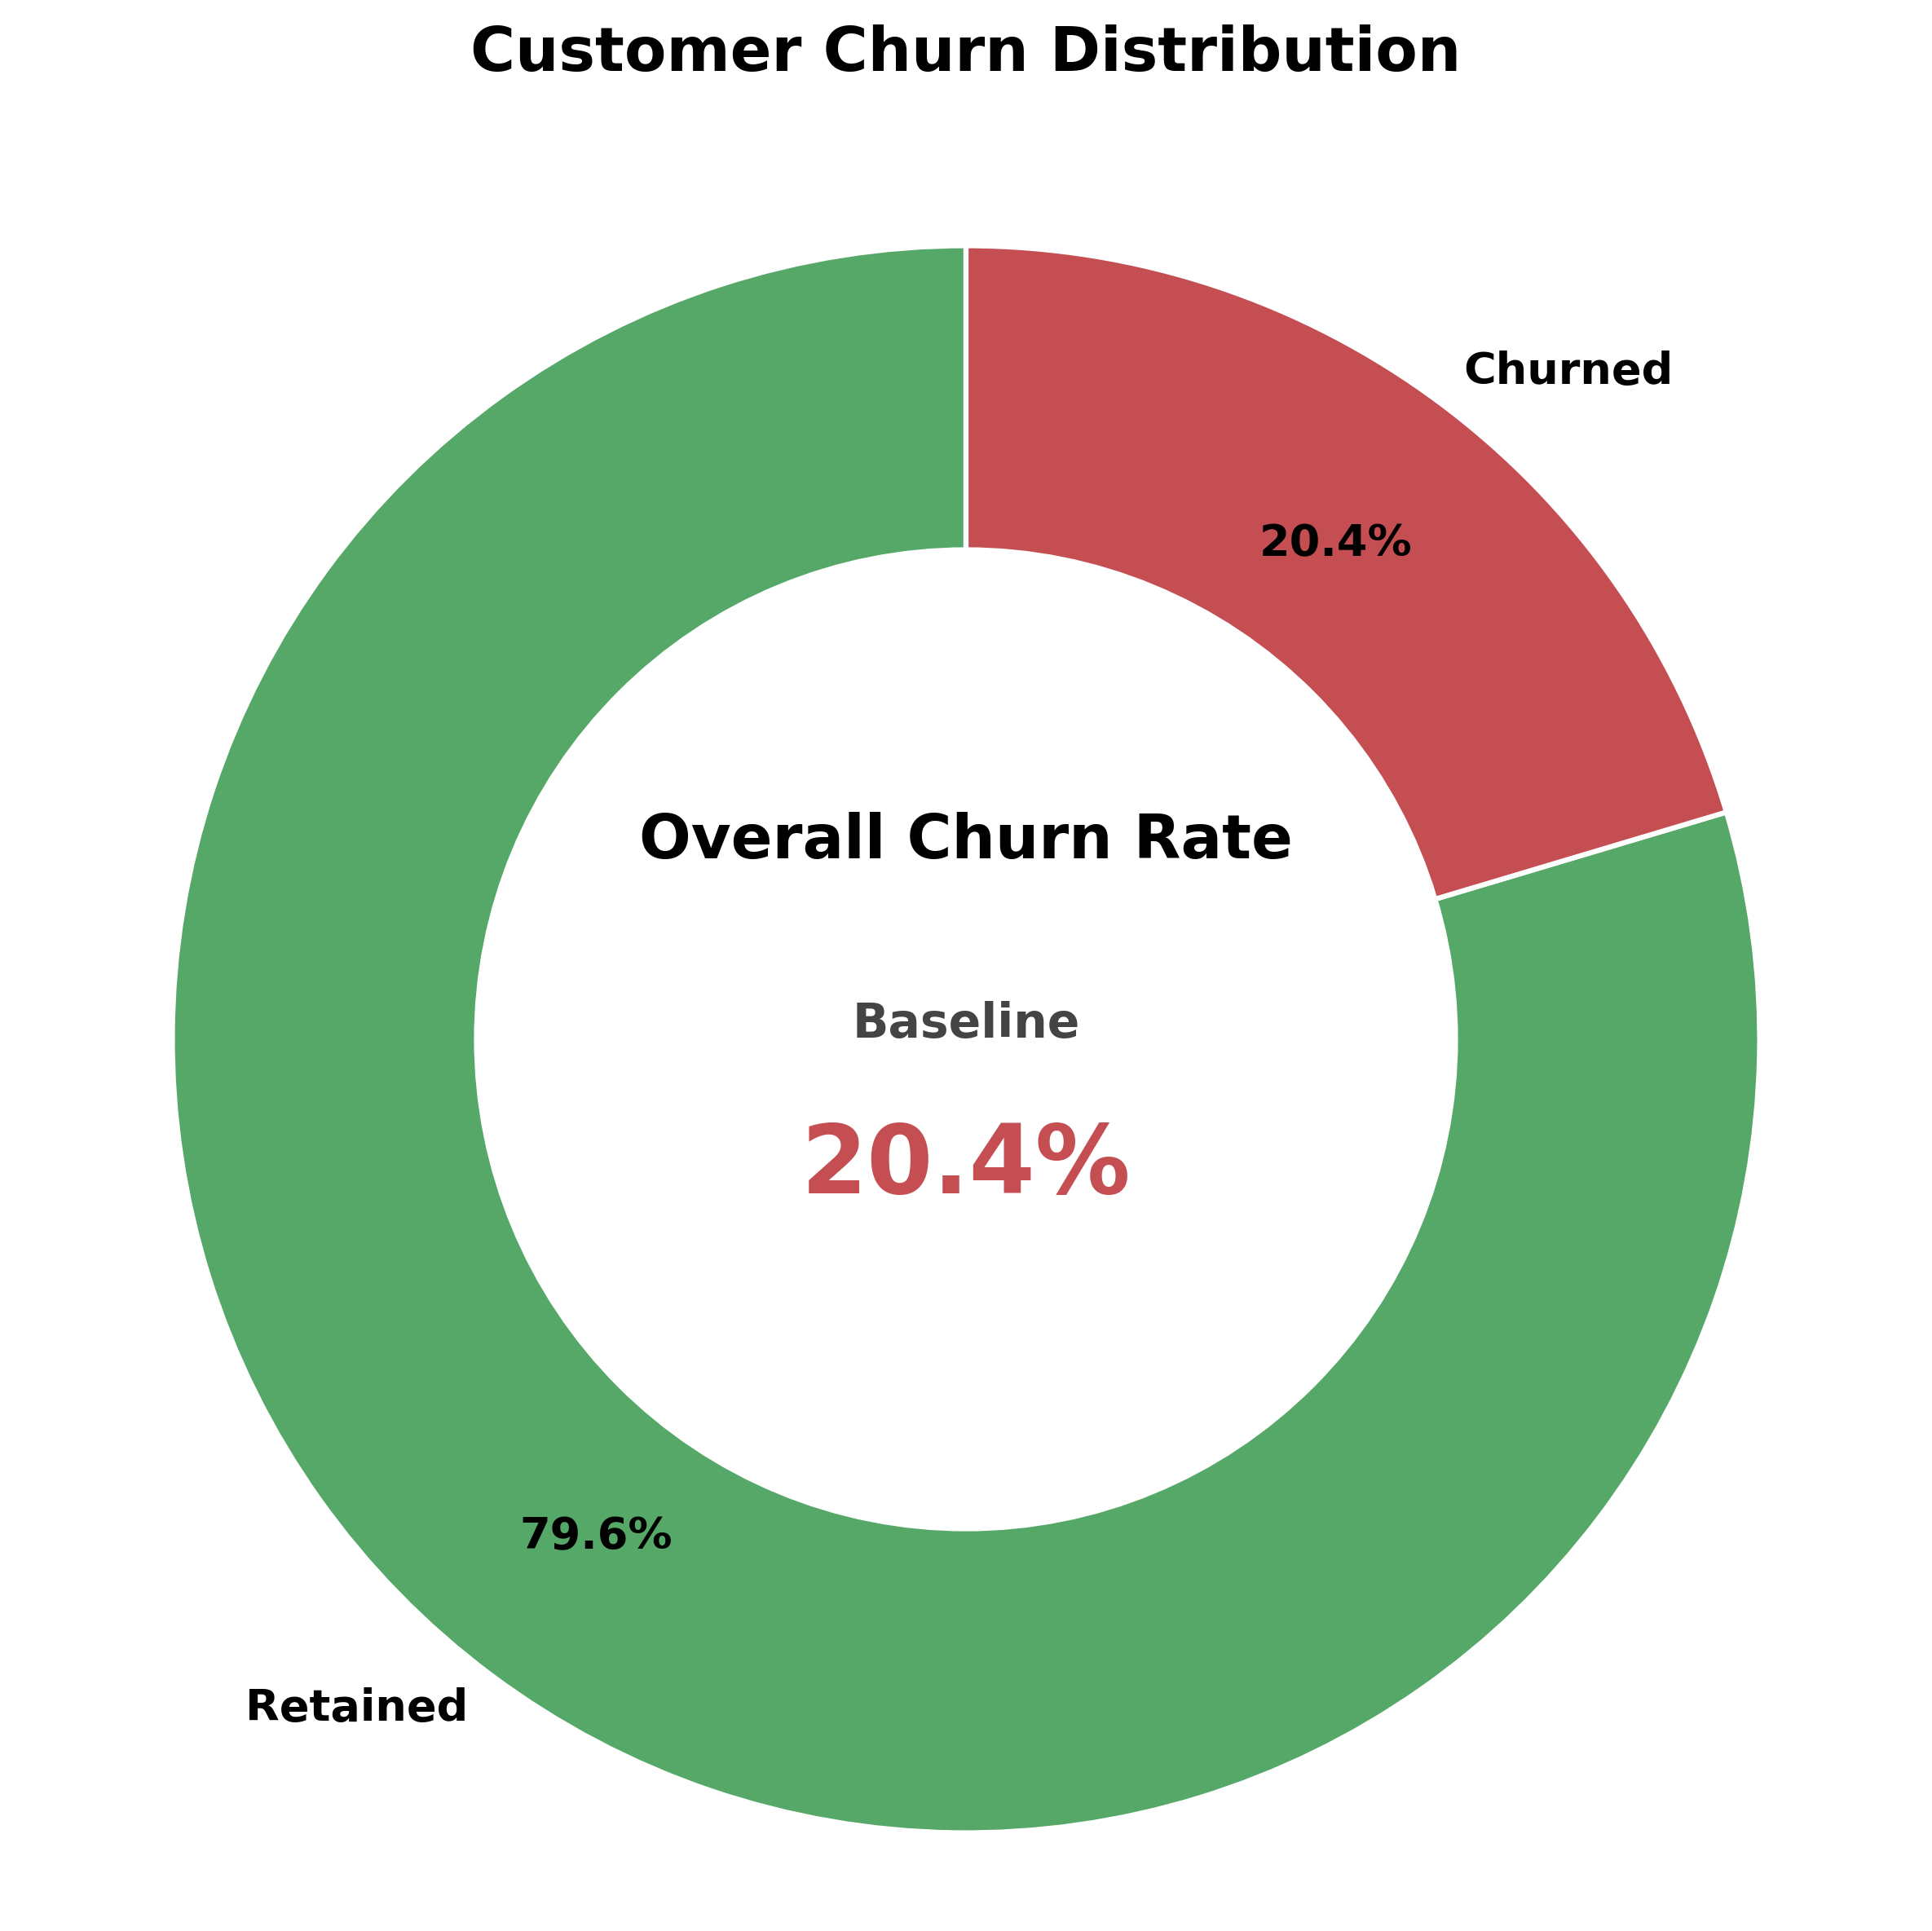
\includegraphics[width=0.5\textwidth]{../img/04_products_donut_chart.png}
\caption{Overall customer churn rate distribution. Baseline churn rate is 20.4\%.}
\label{fig:churn_rate}
\end{figure}

\subsubsection{Segment-Level Churn Patterns}
A "Goldilocks" effect was observed with respect to the number of products owned: customers with exactly two products exhibited the lowest churn rate (7.6~\%, n=4,590), whereas those with three or four products showed higher attrition rates (82.7~\% and 100~\% respectively, n=266 and n=60 respectively), as shown in Figure~\ref{fig:products}. Age displayed a lifecycle pattern, with churn rates rising sharply for pre‑retirement customers (51–60 years) and declining for very young or very old clients (Figure~\ref{fig:age}). Activity status was strongly predictive: inactive members were 1.88 times more likely to churn than active members (Figure~\ref{fig:active}). Geography revealed a pronounced disparity: German customers had twice the churn rate of their French and Spanish counterparts (Figure~\ref{fig:geography}).

\begin{figure}[H]
\centering
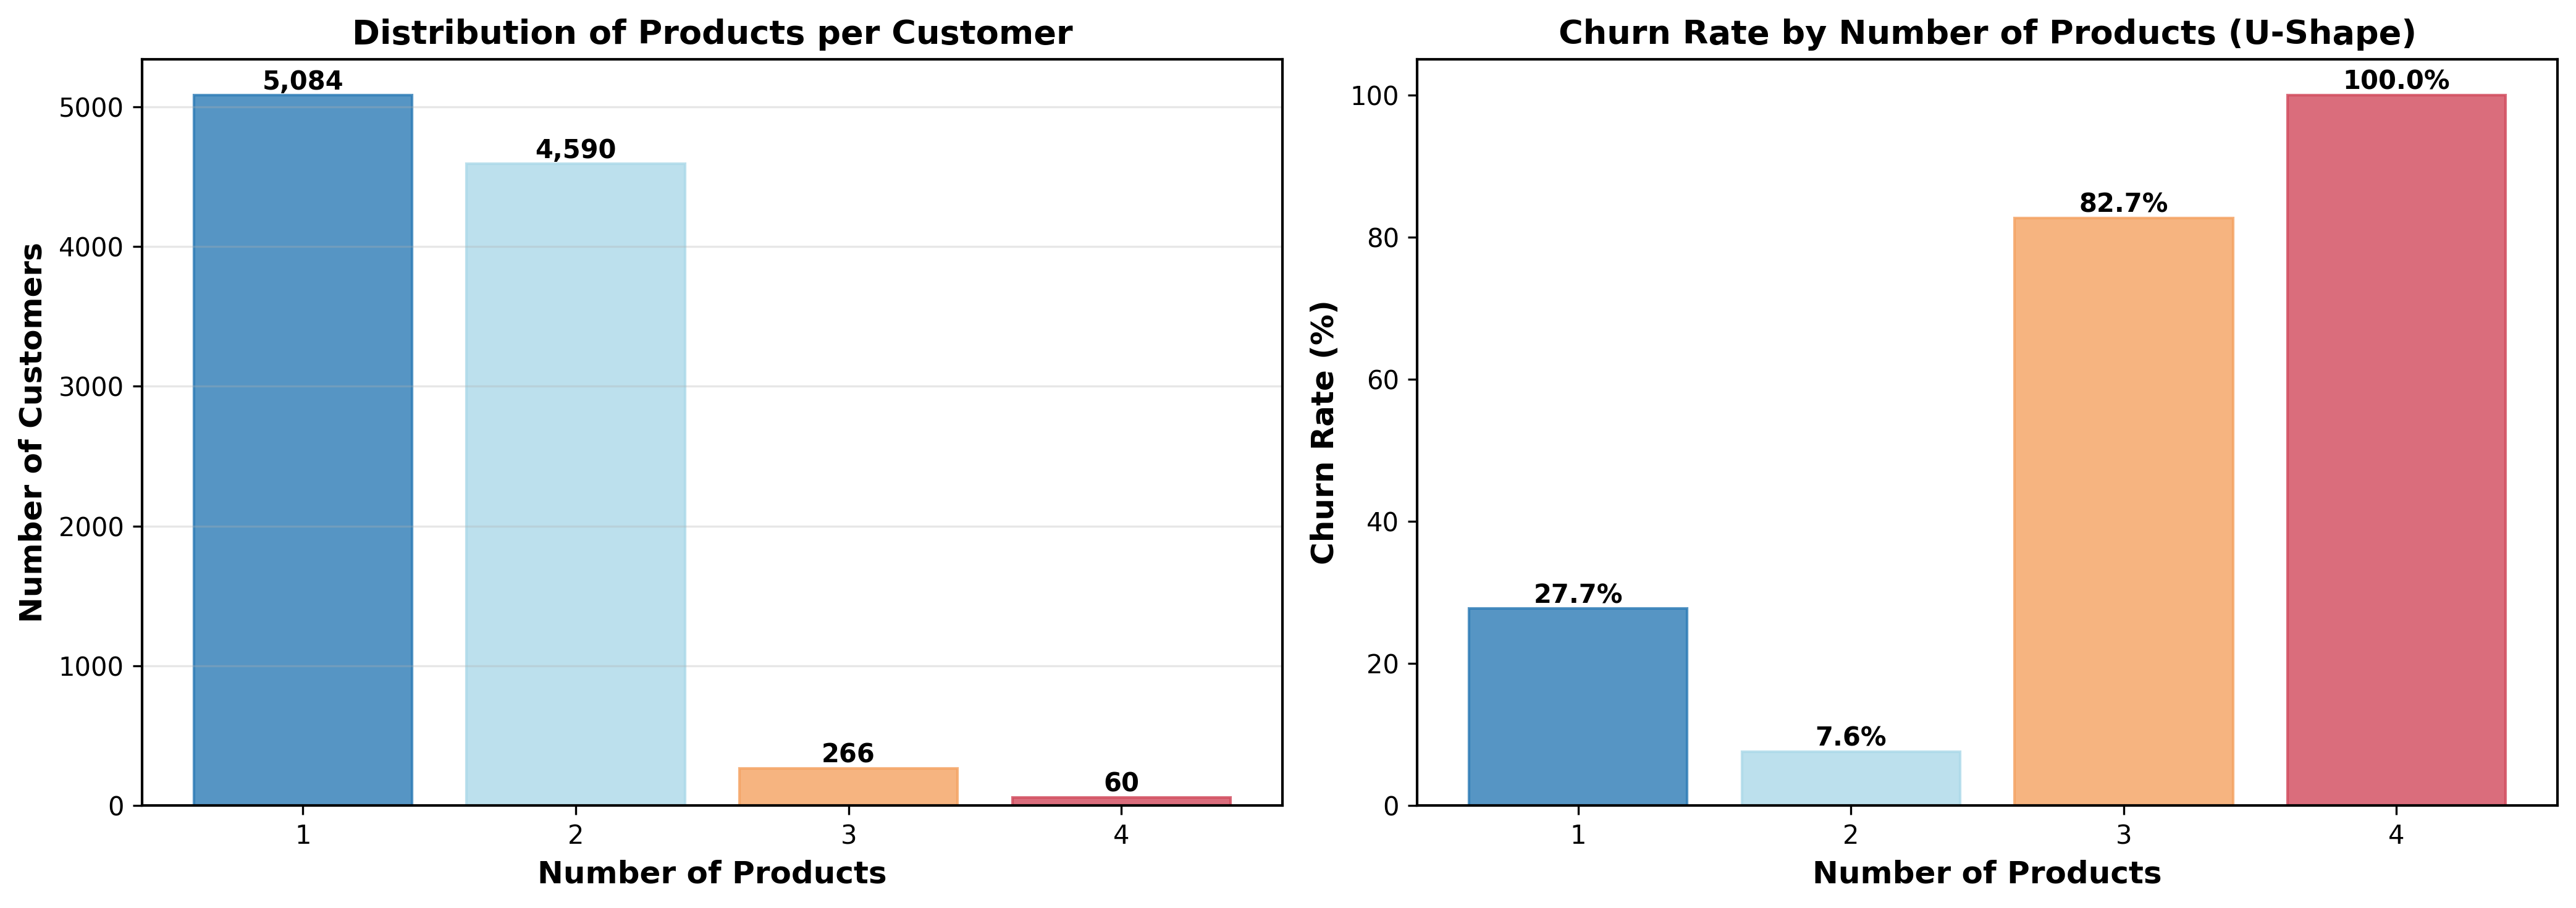
\includegraphics[width=0.7\textwidth]{../img/04_products_churn_analysis.png}
\caption{Product count analysis revealing "Goldilocks" effect. Customers with exactly 2 products show optimal retention.}
\label{fig:products}
\end{figure}

\begin{figure}[H]
\centering
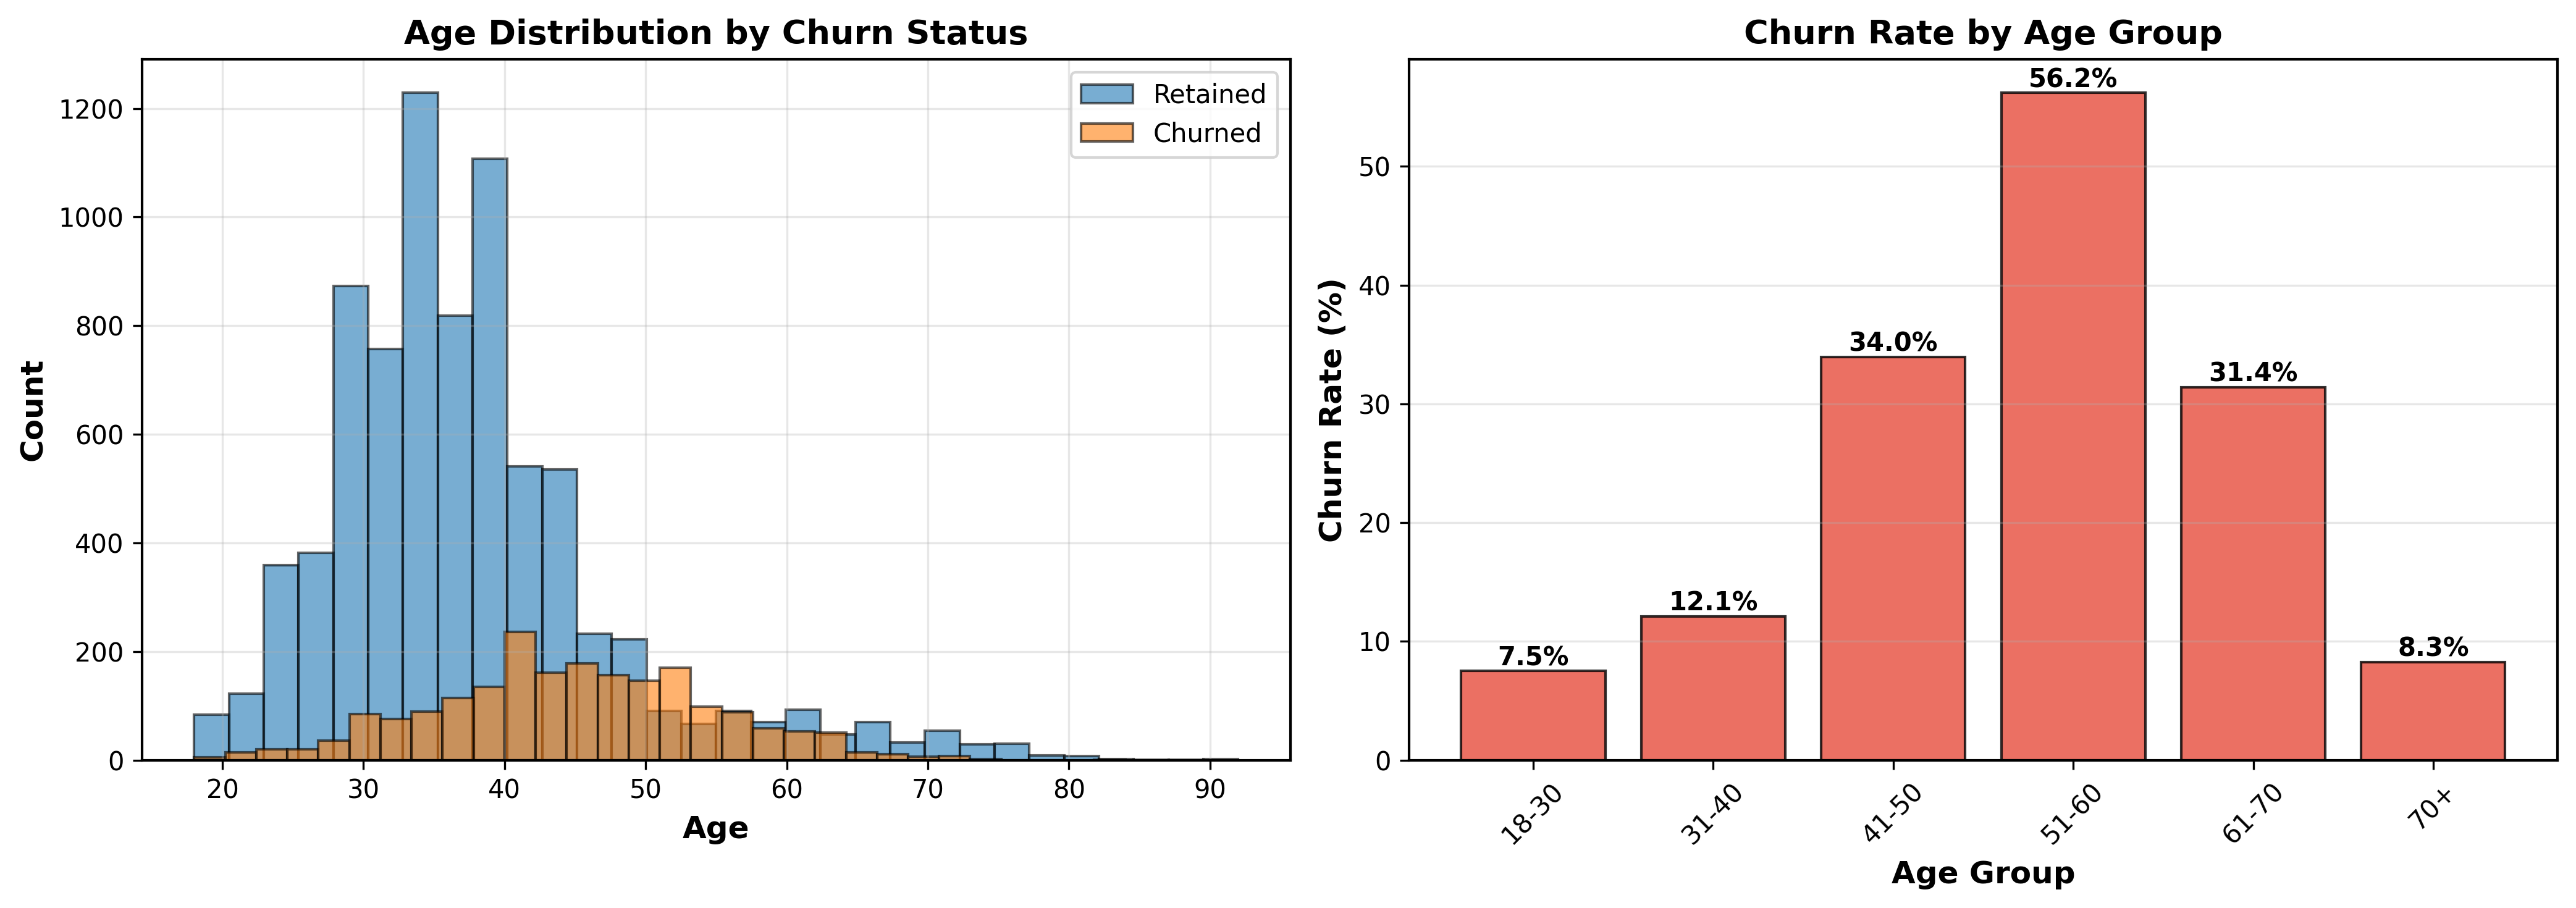
\includegraphics[width=0.7\textwidth]{../img/03_age_distribution_churn.png}
\caption{Age lifecycle pattern in churn risk. Peak vulnerability occurs at 51–60 years.}
\label{fig:age}
\end{figure}

\begin{figure}[H]
\centering
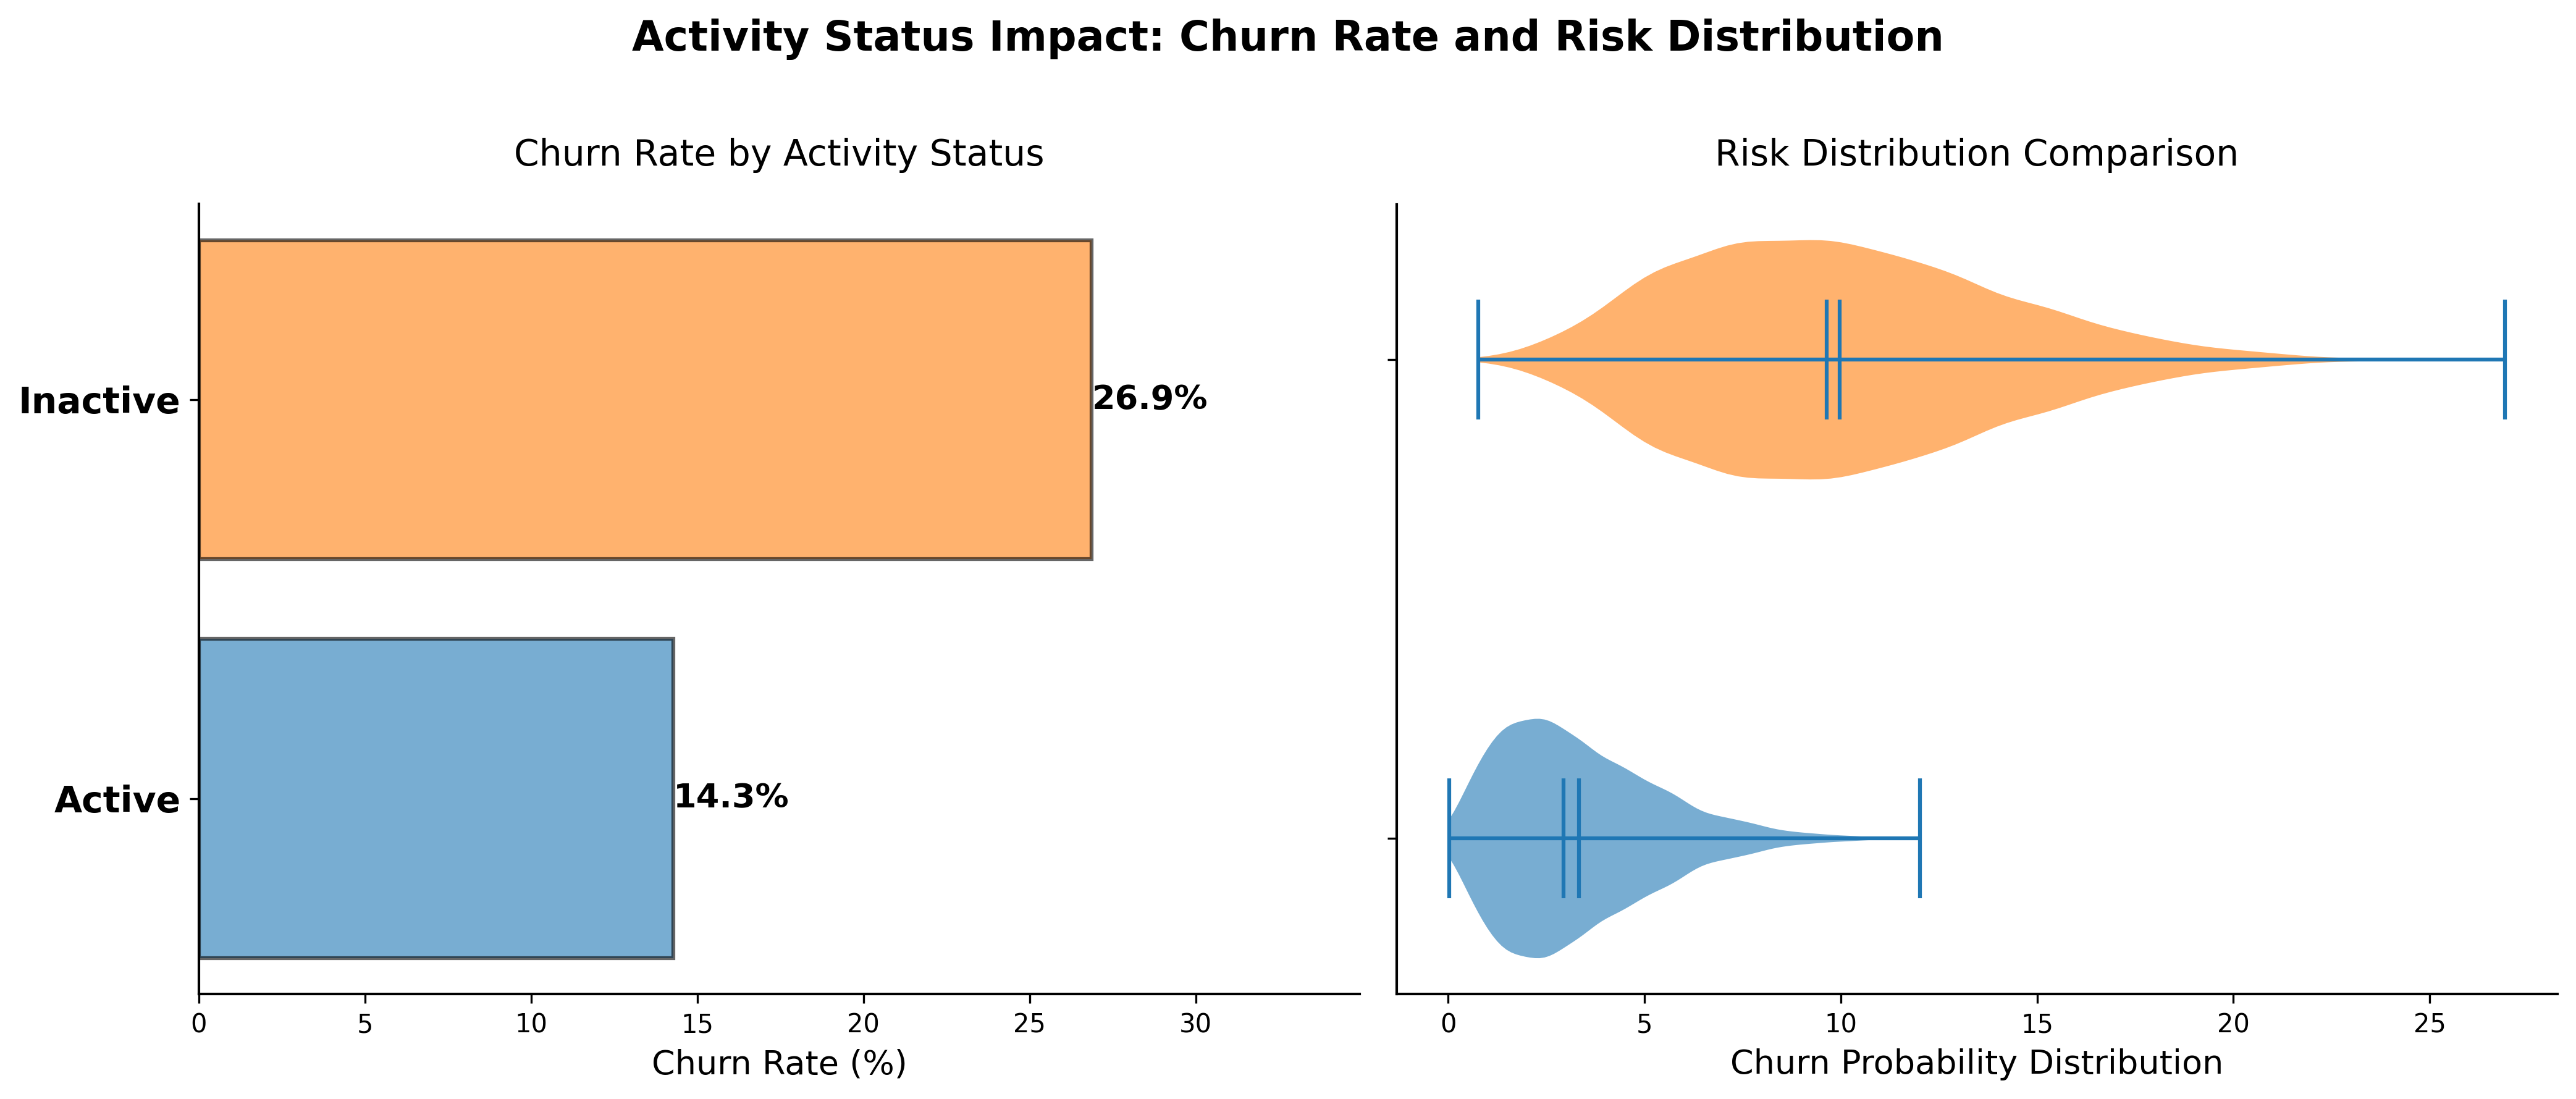
\includegraphics[width=0.9\textwidth]{../img/08_churn_rate_violin_hybridv2.png}
\caption{Activity status impact on churn risk. Inactive members exhibit 1.88× higher churn risk than active members.}
\label{fig:active}
\end{figure}

\begin{figure}[H]
\centering
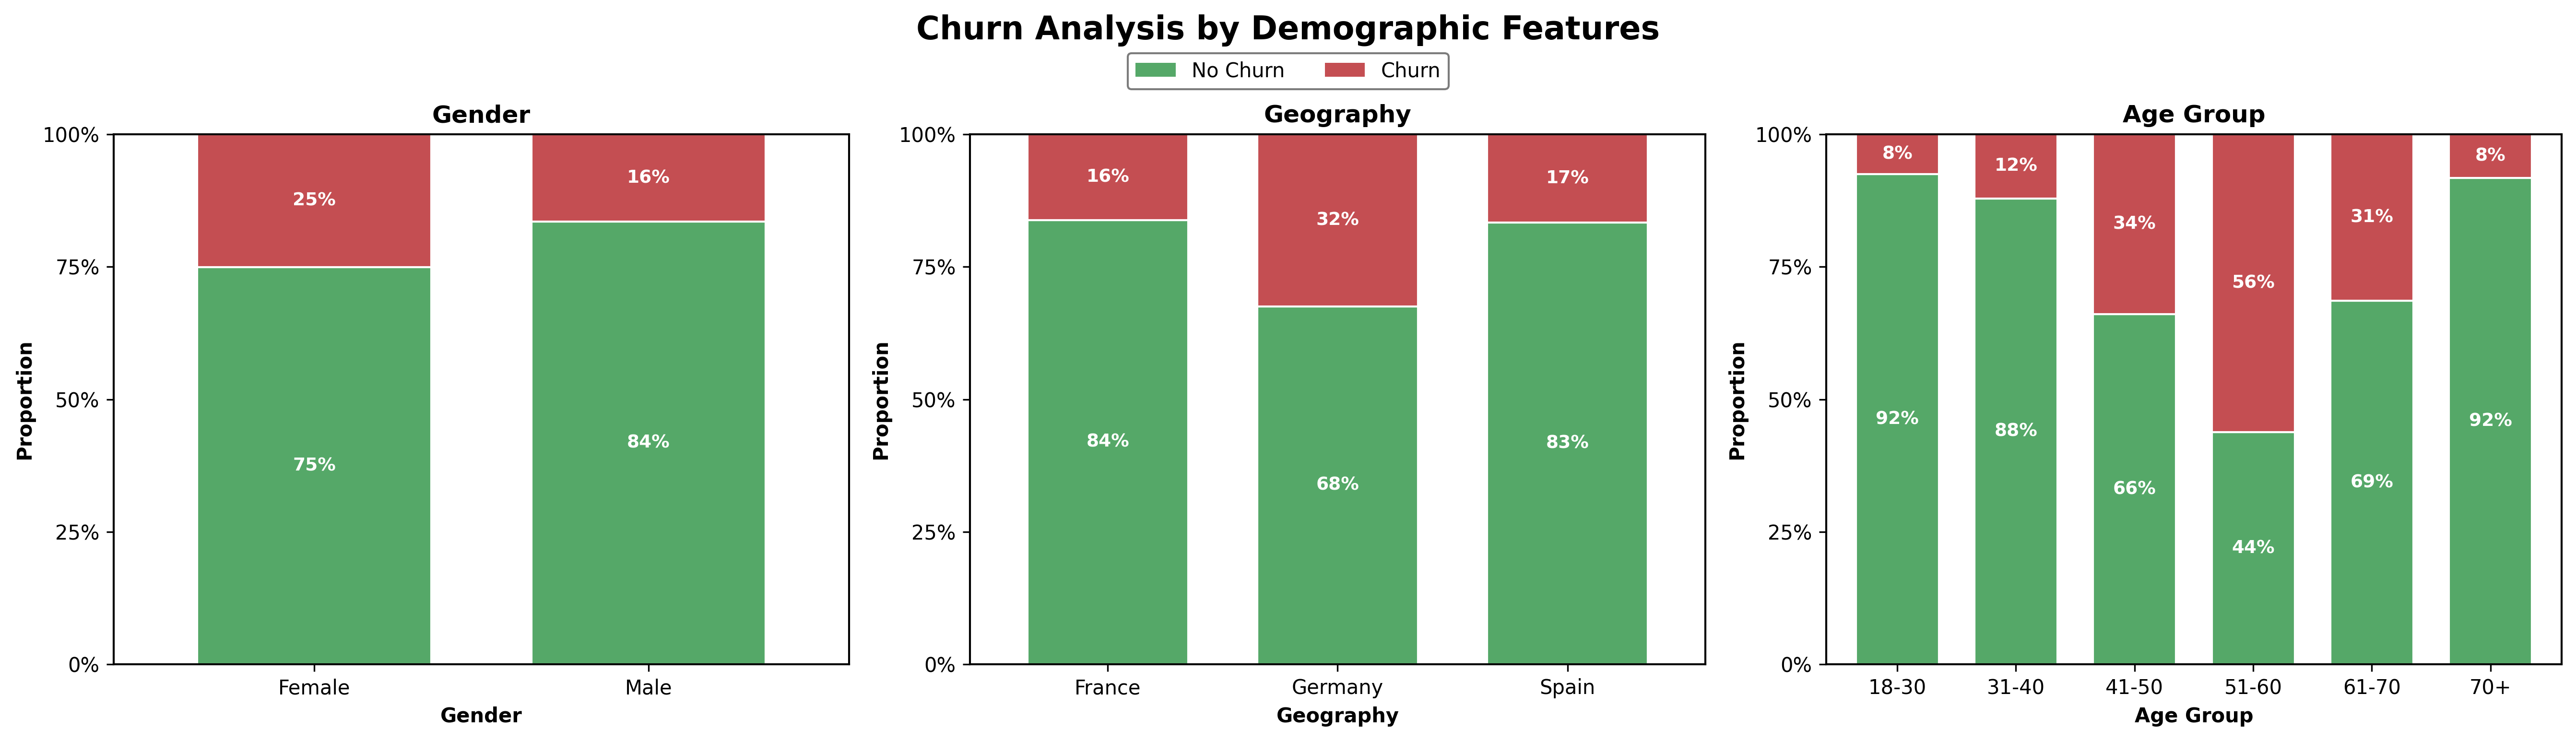
\includegraphics[width=0.9\textwidth]{../img/02_demographic_overview.png}
\caption{Demographic overview showing geographic churn disparity. Germany exhibits churn rates 2× higher than France and Spain.}
\label{fig:geography}
\end{figure}

\subsubsection{Feature Selection Analysis}
Linear correlation analysis with churn revealed distinct tiers of predictive strength (Figure~\ref{fig:feature_selection}). Age, activity status and balance showed moderate to strong correlations (r=0.285, -0.156 and 0.119 respectively) and were retained as core predictors, along with geography and number of products. In contrast, satisfaction\_score, point\_earned, estimated\_salary, credit\_score, tenure and card\_type exhibited minimal linear relationships (|r| $<$ 0.10) and were excluded from modeling.

\begin{figure}[H]
\centering
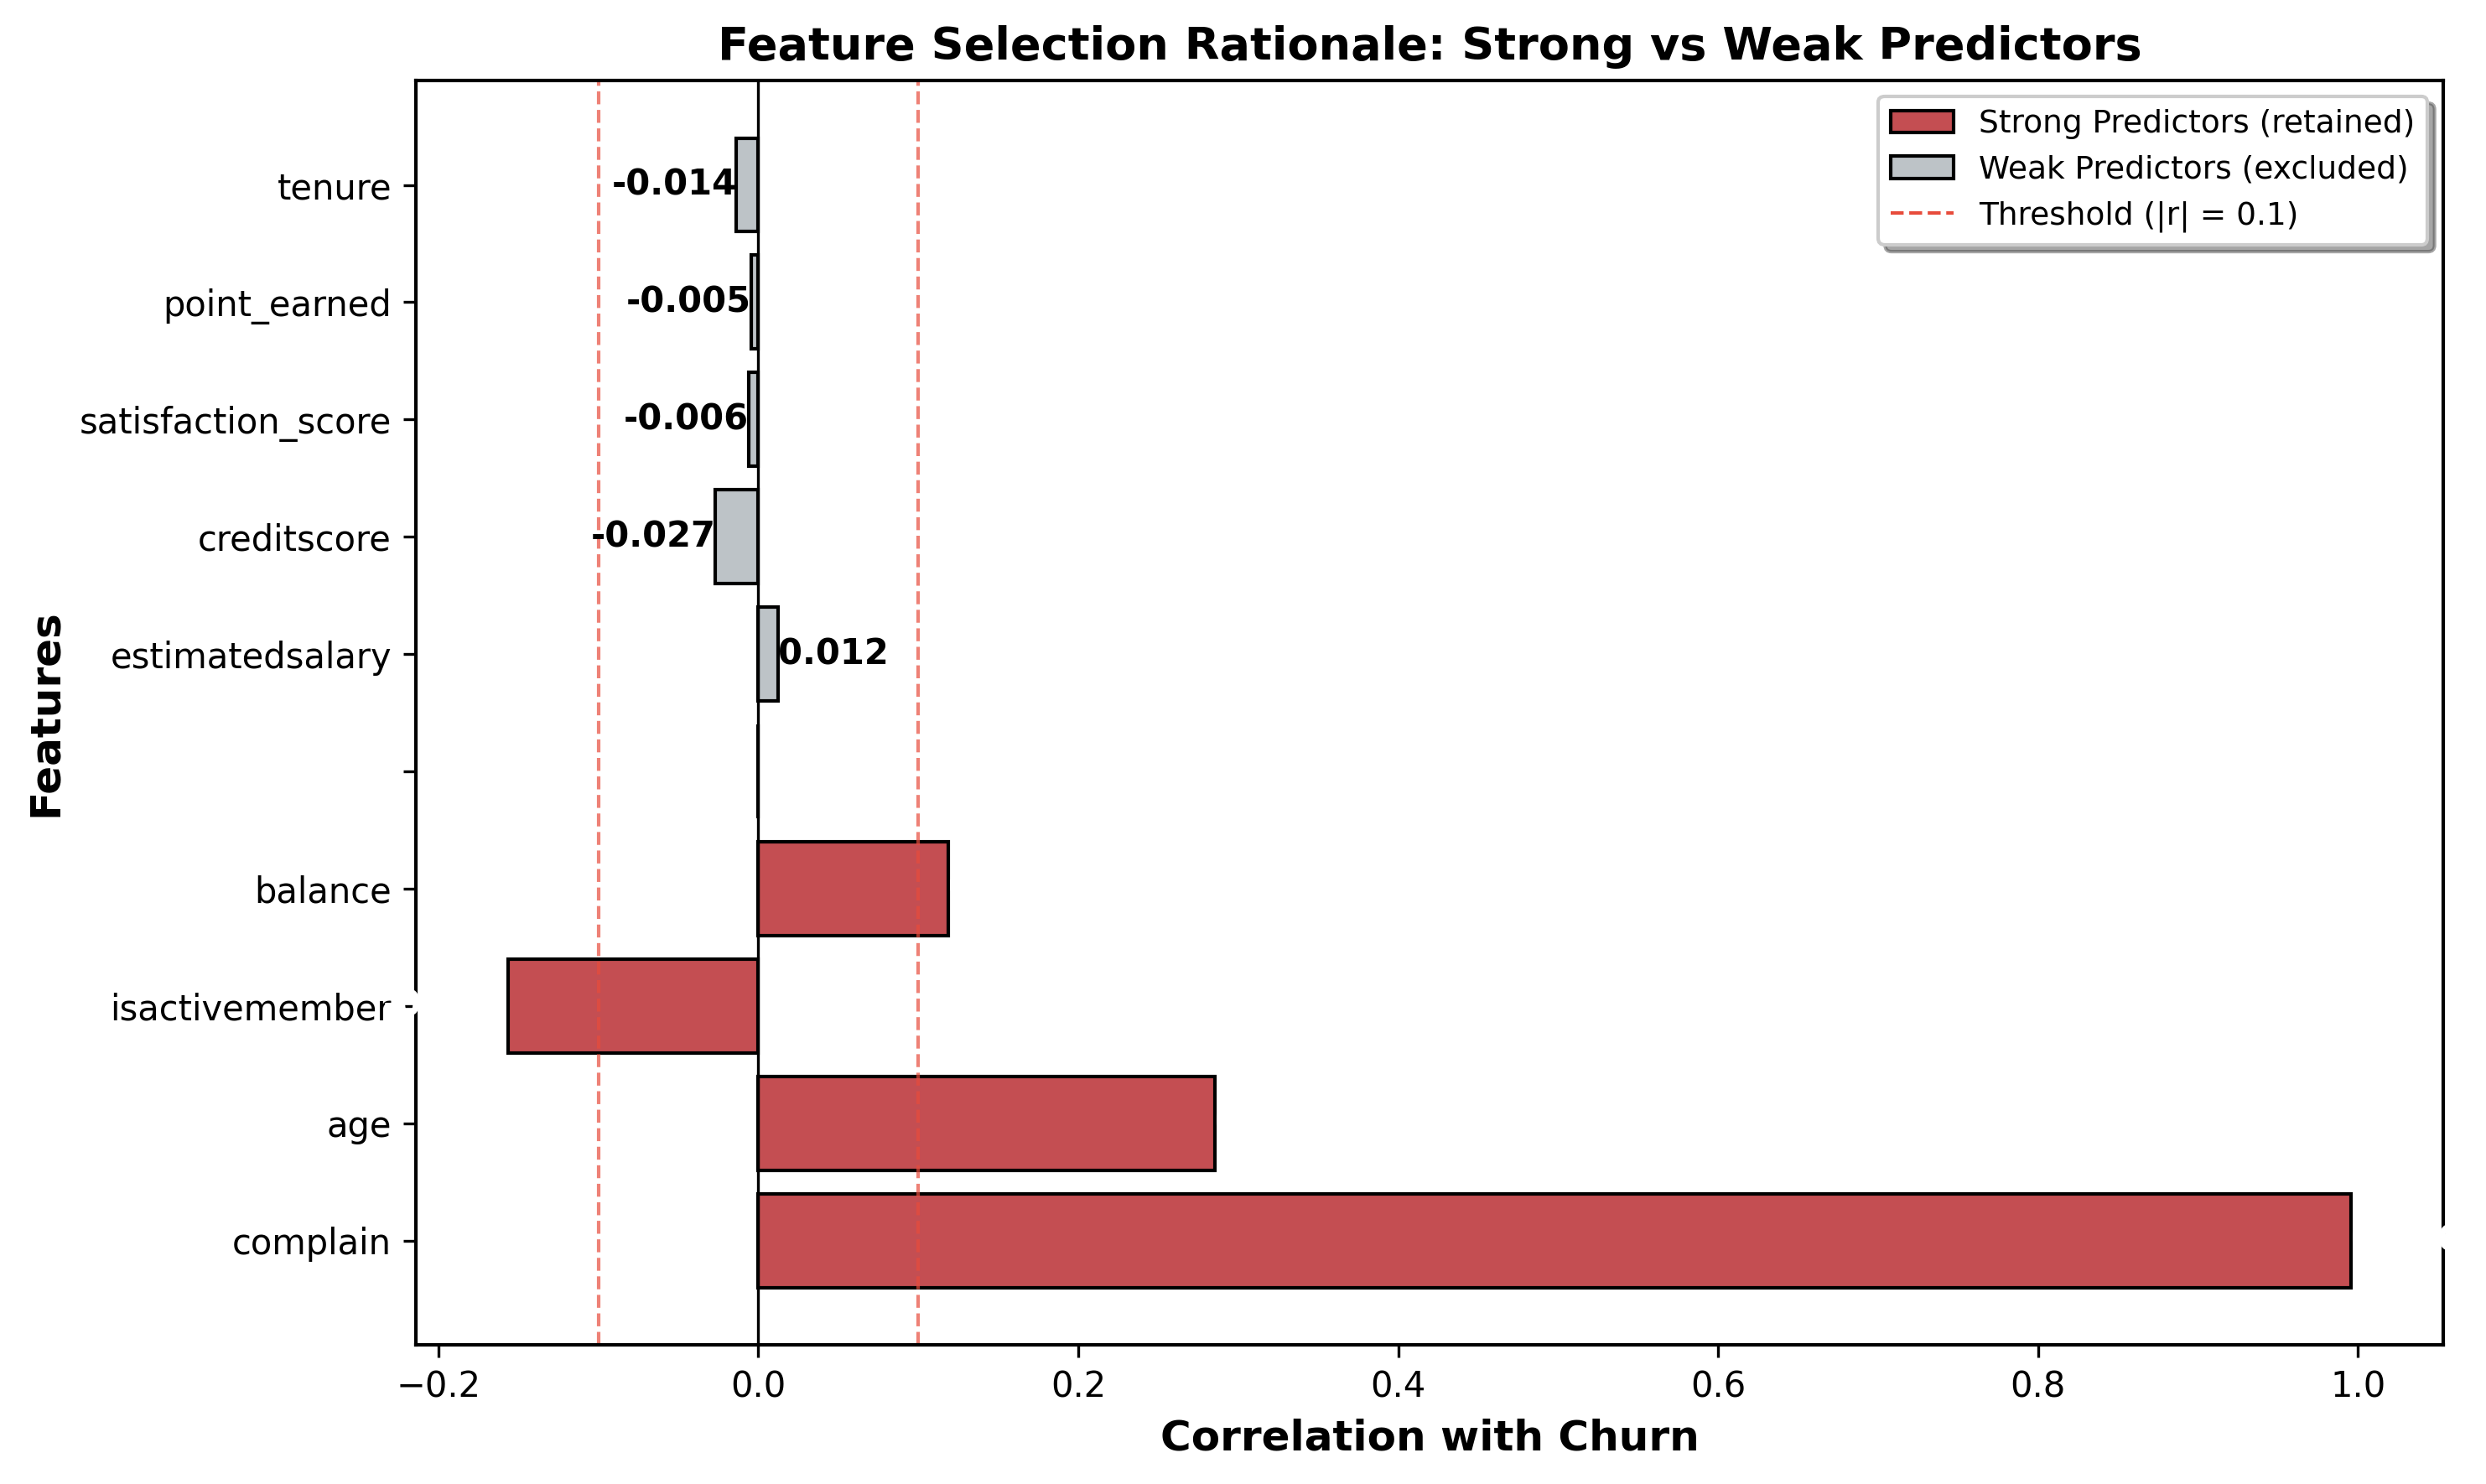
\includegraphics[width=0.7\textwidth]{../img/feature_selection_comparison.png}
\caption{Feature selection rationale comparing strong (|r| $\geq$ 0.10) and weak (|r| $<$ 0.10) predictors. Strong predictors (red) were retained for modeling; weak predictors (gray) were excluded. Complaint status shows near‑perfect correlation (r=0.996) but is excluded as a lagging indicator.}
\label{fig:feature_selection}
\end{figure}

While including complaint status would yield near‑perfect accuracy (99\%+), it represents a methodological degenerate case: the model achieves inflated performance by relying on a single dominant feature that essentially solves the classification problem before meaningful pattern recognition occurs. Following best practices in operational ML \citep{kumar2022customerretention}, complaint status was intentionally excluded to enable genuine feature discovery and actionable business intelligence. This trade-off sacrifices headline accuracy metrics (85.9\% vs.\ potential 99\%+) to uncover meaningful antecedent patterns that drive real intervention strategies. Models achieving high accuracy through lagging indicators identify customers who have already expressed dissatisfaction through formal channels, exactly when retention is least likely to succeed.

Kernel density estimates for excluded continuous features (Figure~\ref{fig:kde_weak}) confirm their lack of discriminatory power through near‑complete distributional overlap between churned and retained customers. Similar minimal effects were observed for categorical excluded features: card type exhibited only a 2.5 percentage point difference in churn rates across all four tiers (19.3\%–21.8\%). Notably, the number of products showed weak linear correlation (r=-0.048) but was retained based on its demonstrated non‑linear U‑shaped effect. This feature selection framework maintains predictive power through tree‑based algorithms capable of capturing non‑linear relationships while prioritizing interpretability.

\begin{figure}[H]
\centering
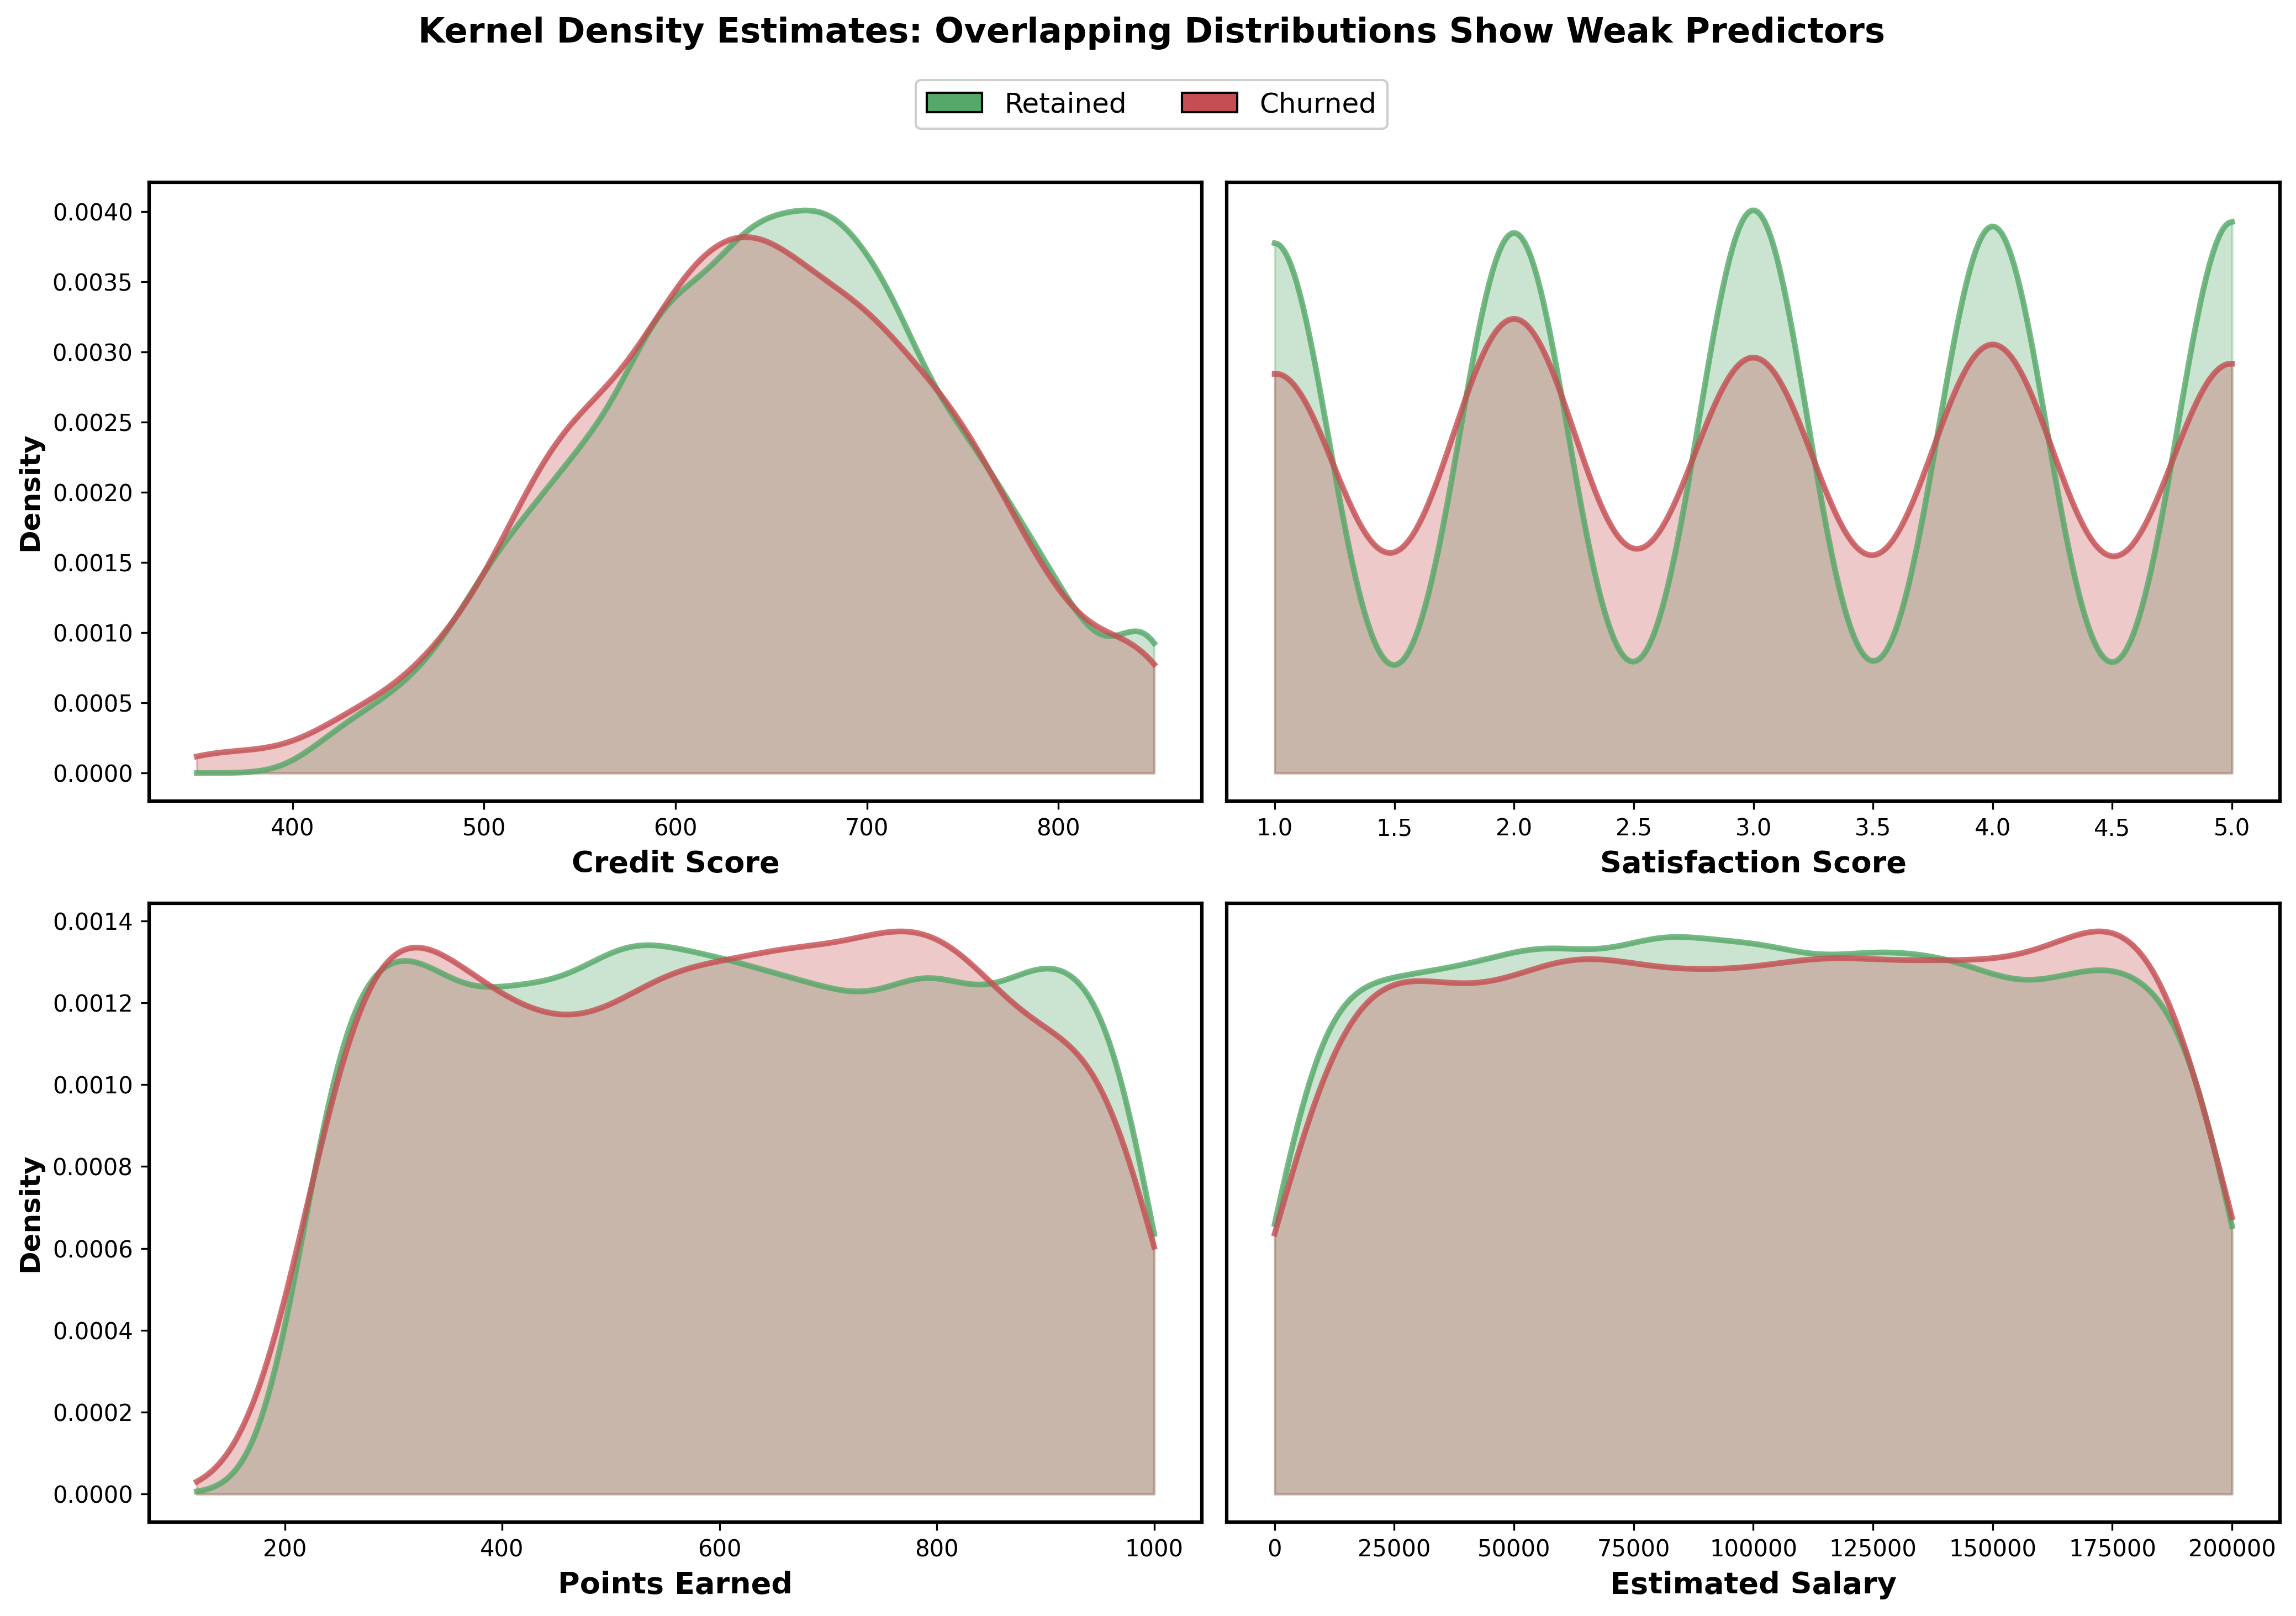
\includegraphics[width=0.75\textwidth]{../img/poc_kde_plots.png}
\caption{Kernel density estimates for excluded continuous features. Near‑complete overlap between churned (red) and retained (green) distributions confirms these features lack discriminatory power, visually validating their weak correlation values.}
\label{fig:kde_weak}
\end{figure}

Pearson correlation analysis (Figure~\ref{fig:correlation}) revealed non‑linear patterns, particularly for the number of products (a U‑shaped relationship) and complex associations between age and activity status.

\begin{figure}[H]
\centering
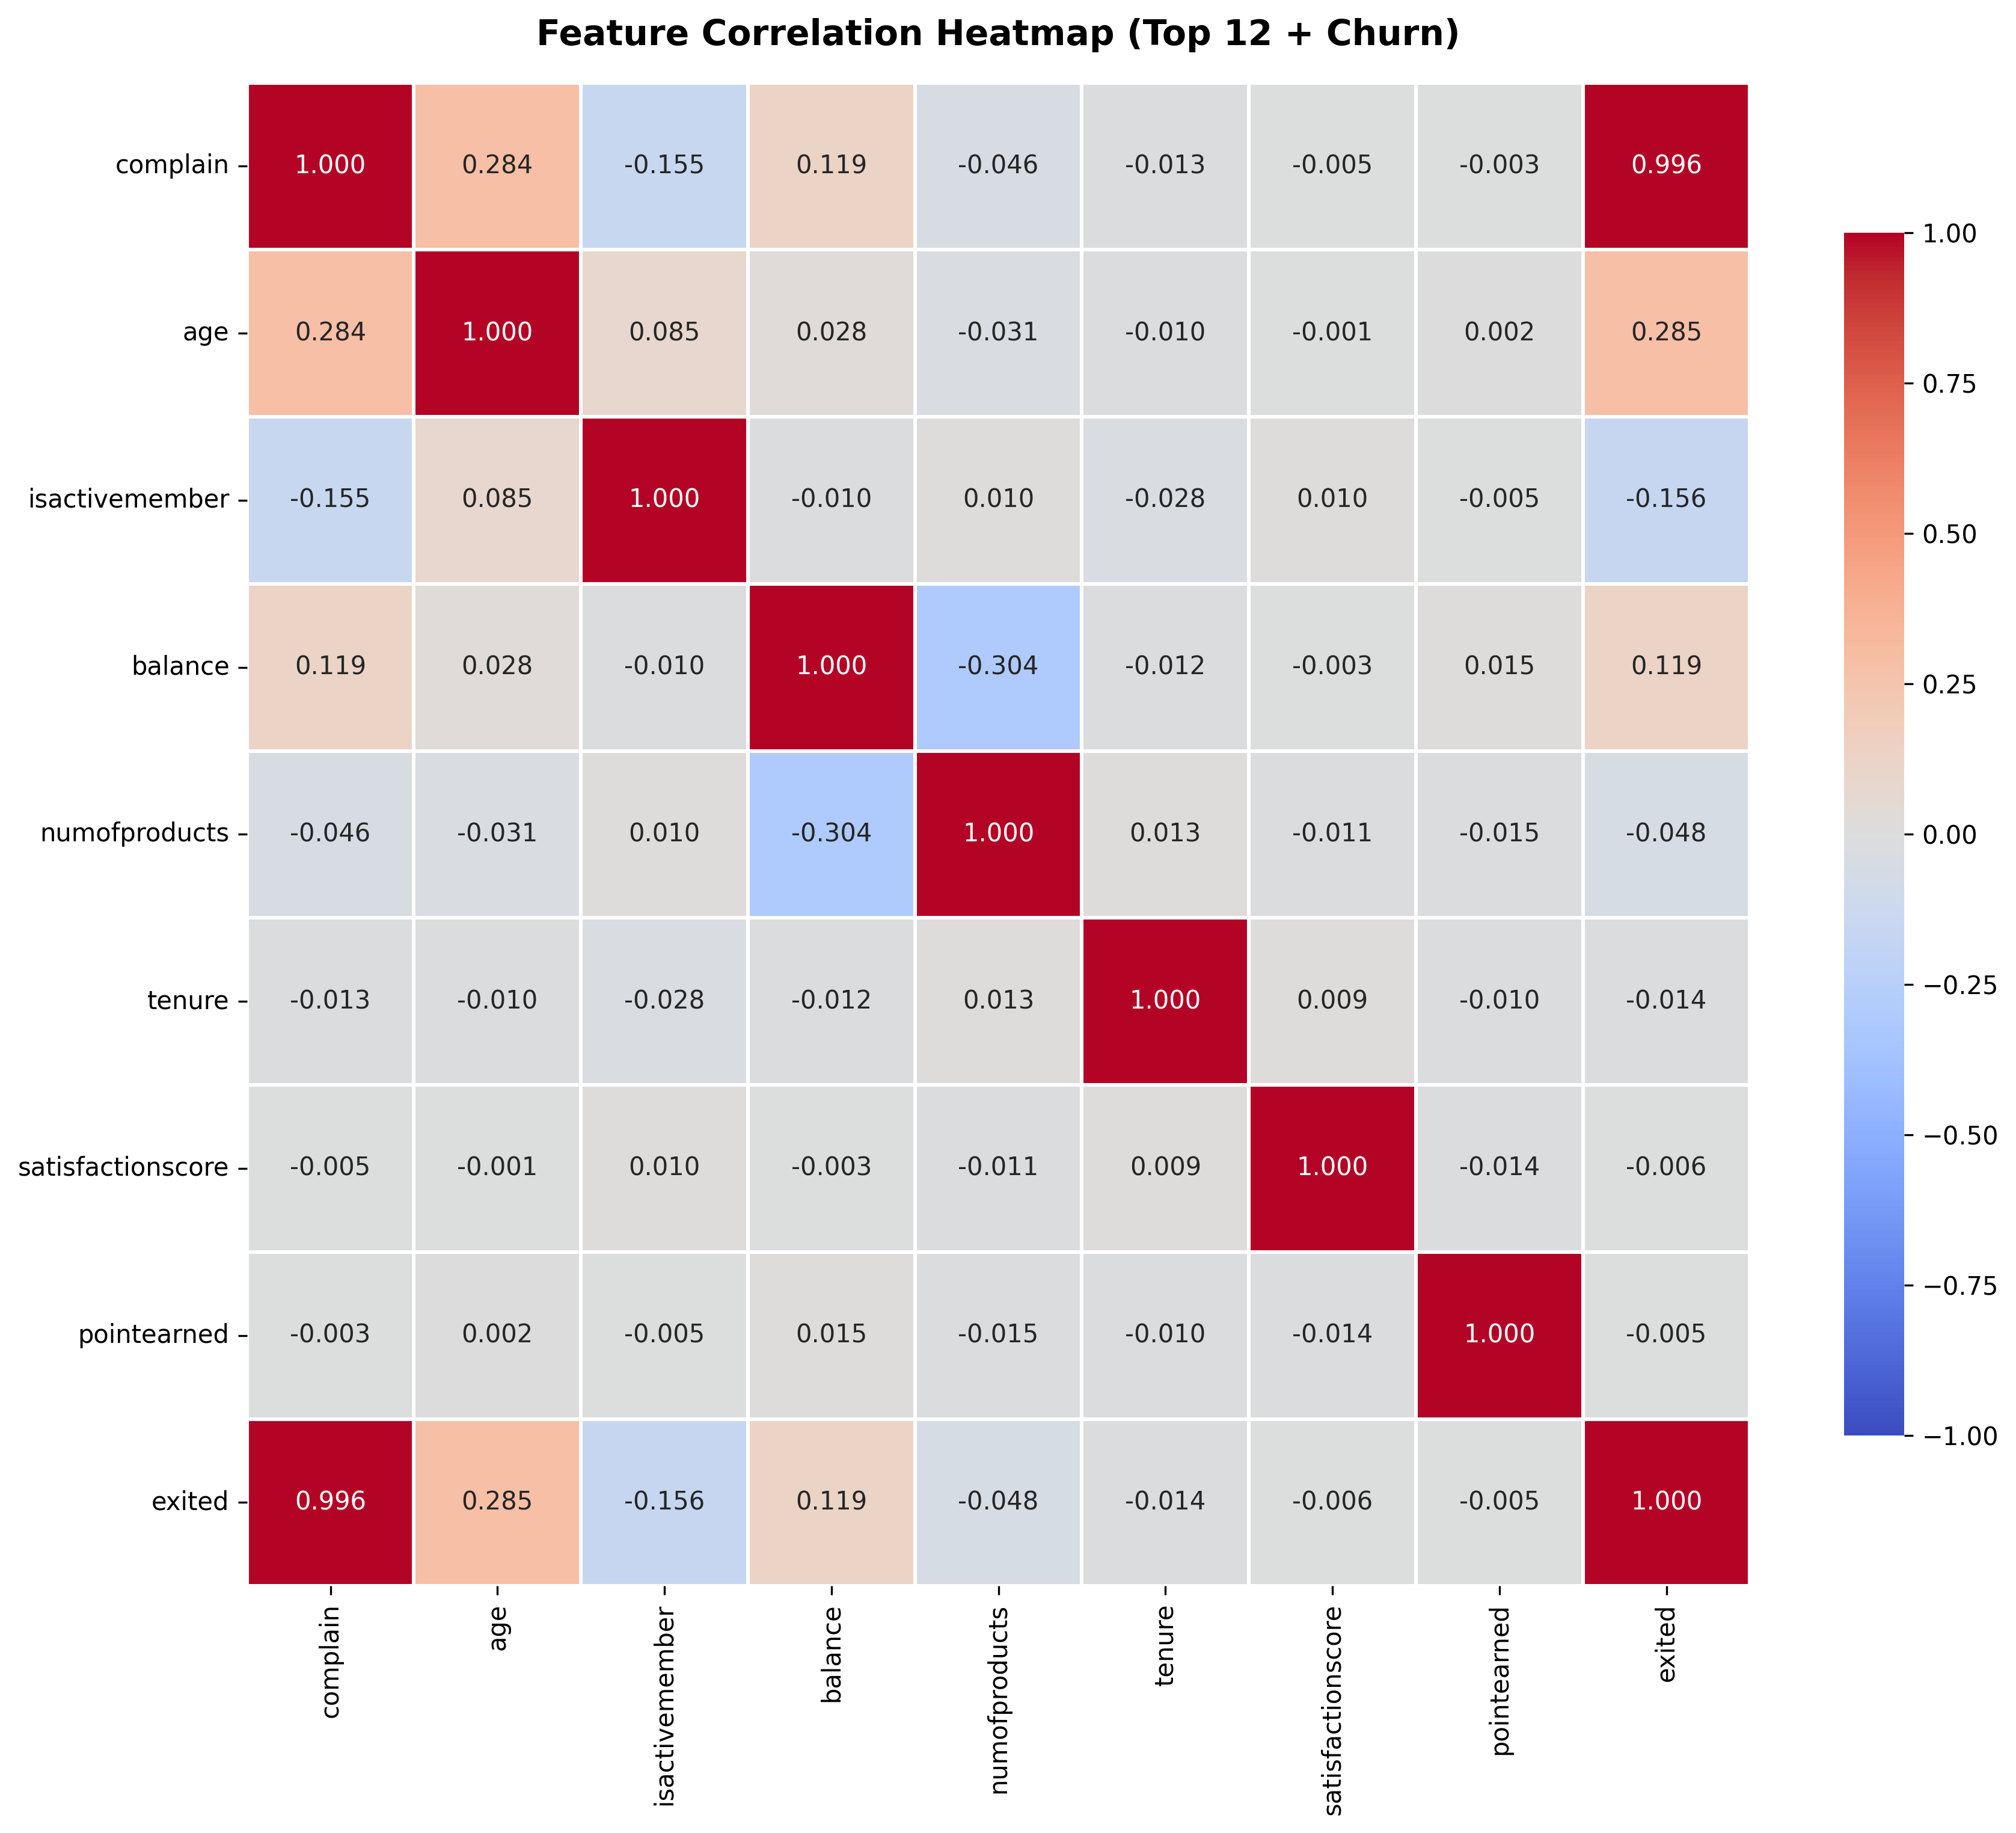
\includegraphics[width=0.8\textwidth]{../img/08_correlation_heatmap.png}
\caption{Feature correlation heatmap. Complaint status shows near‑perfect correlation with churn (r=0.996). Moderate correlations exist for age, number of products, and activity status.}
\label{fig:correlation}
\end{figure}

\subsection{Survival Analysis Results}
Survival analysis was conducted to quantify temporal churn patterns and identify risk factors associated with customer attrition over time. Two complementary approaches were employed: non-parametric Kaplan–Meier estimators for univariate analysis and semiparametric Cox proportional hazards regression for multivariate risk assessment.

\subsubsection{Kaplan–Meier Survival Curves}
Kaplan–Meier curves were computed for various customer segments (Figure~\ref{fig:survival_all}). The overall survival curve (Figure~\ref{fig:survival_overall}) indicated that median customer lifetime (time until exit) exceeded 10 years of tenure for the majority of customers. Survival curves by number of products (Figure~\ref{fig:survival_products}) confirmed the U‑shaped pattern; customers with two products had the highest survival, while those with three or four products experienced steep declines. Note that the 3‑product group (n=266) and 4‑product group (n=60) have smaller sample sizes, making their survival curves less precise than those for 1‑product (n=5,084) and 2‑product (n=4,590) groups. Age group curves (Figure~\ref{fig:survival_age}) revealed that pre‑retirement customers (51–60) had the steepest decline, consistent with the lifecycle hypothesis. Activity status curves (Figure~\ref{fig:survival_active}) showed that active members maintained higher survival probabilities over time.

\begin{figure}[H]
\centering
\begin{subfigure}[b]{0.48\textwidth}
\centering
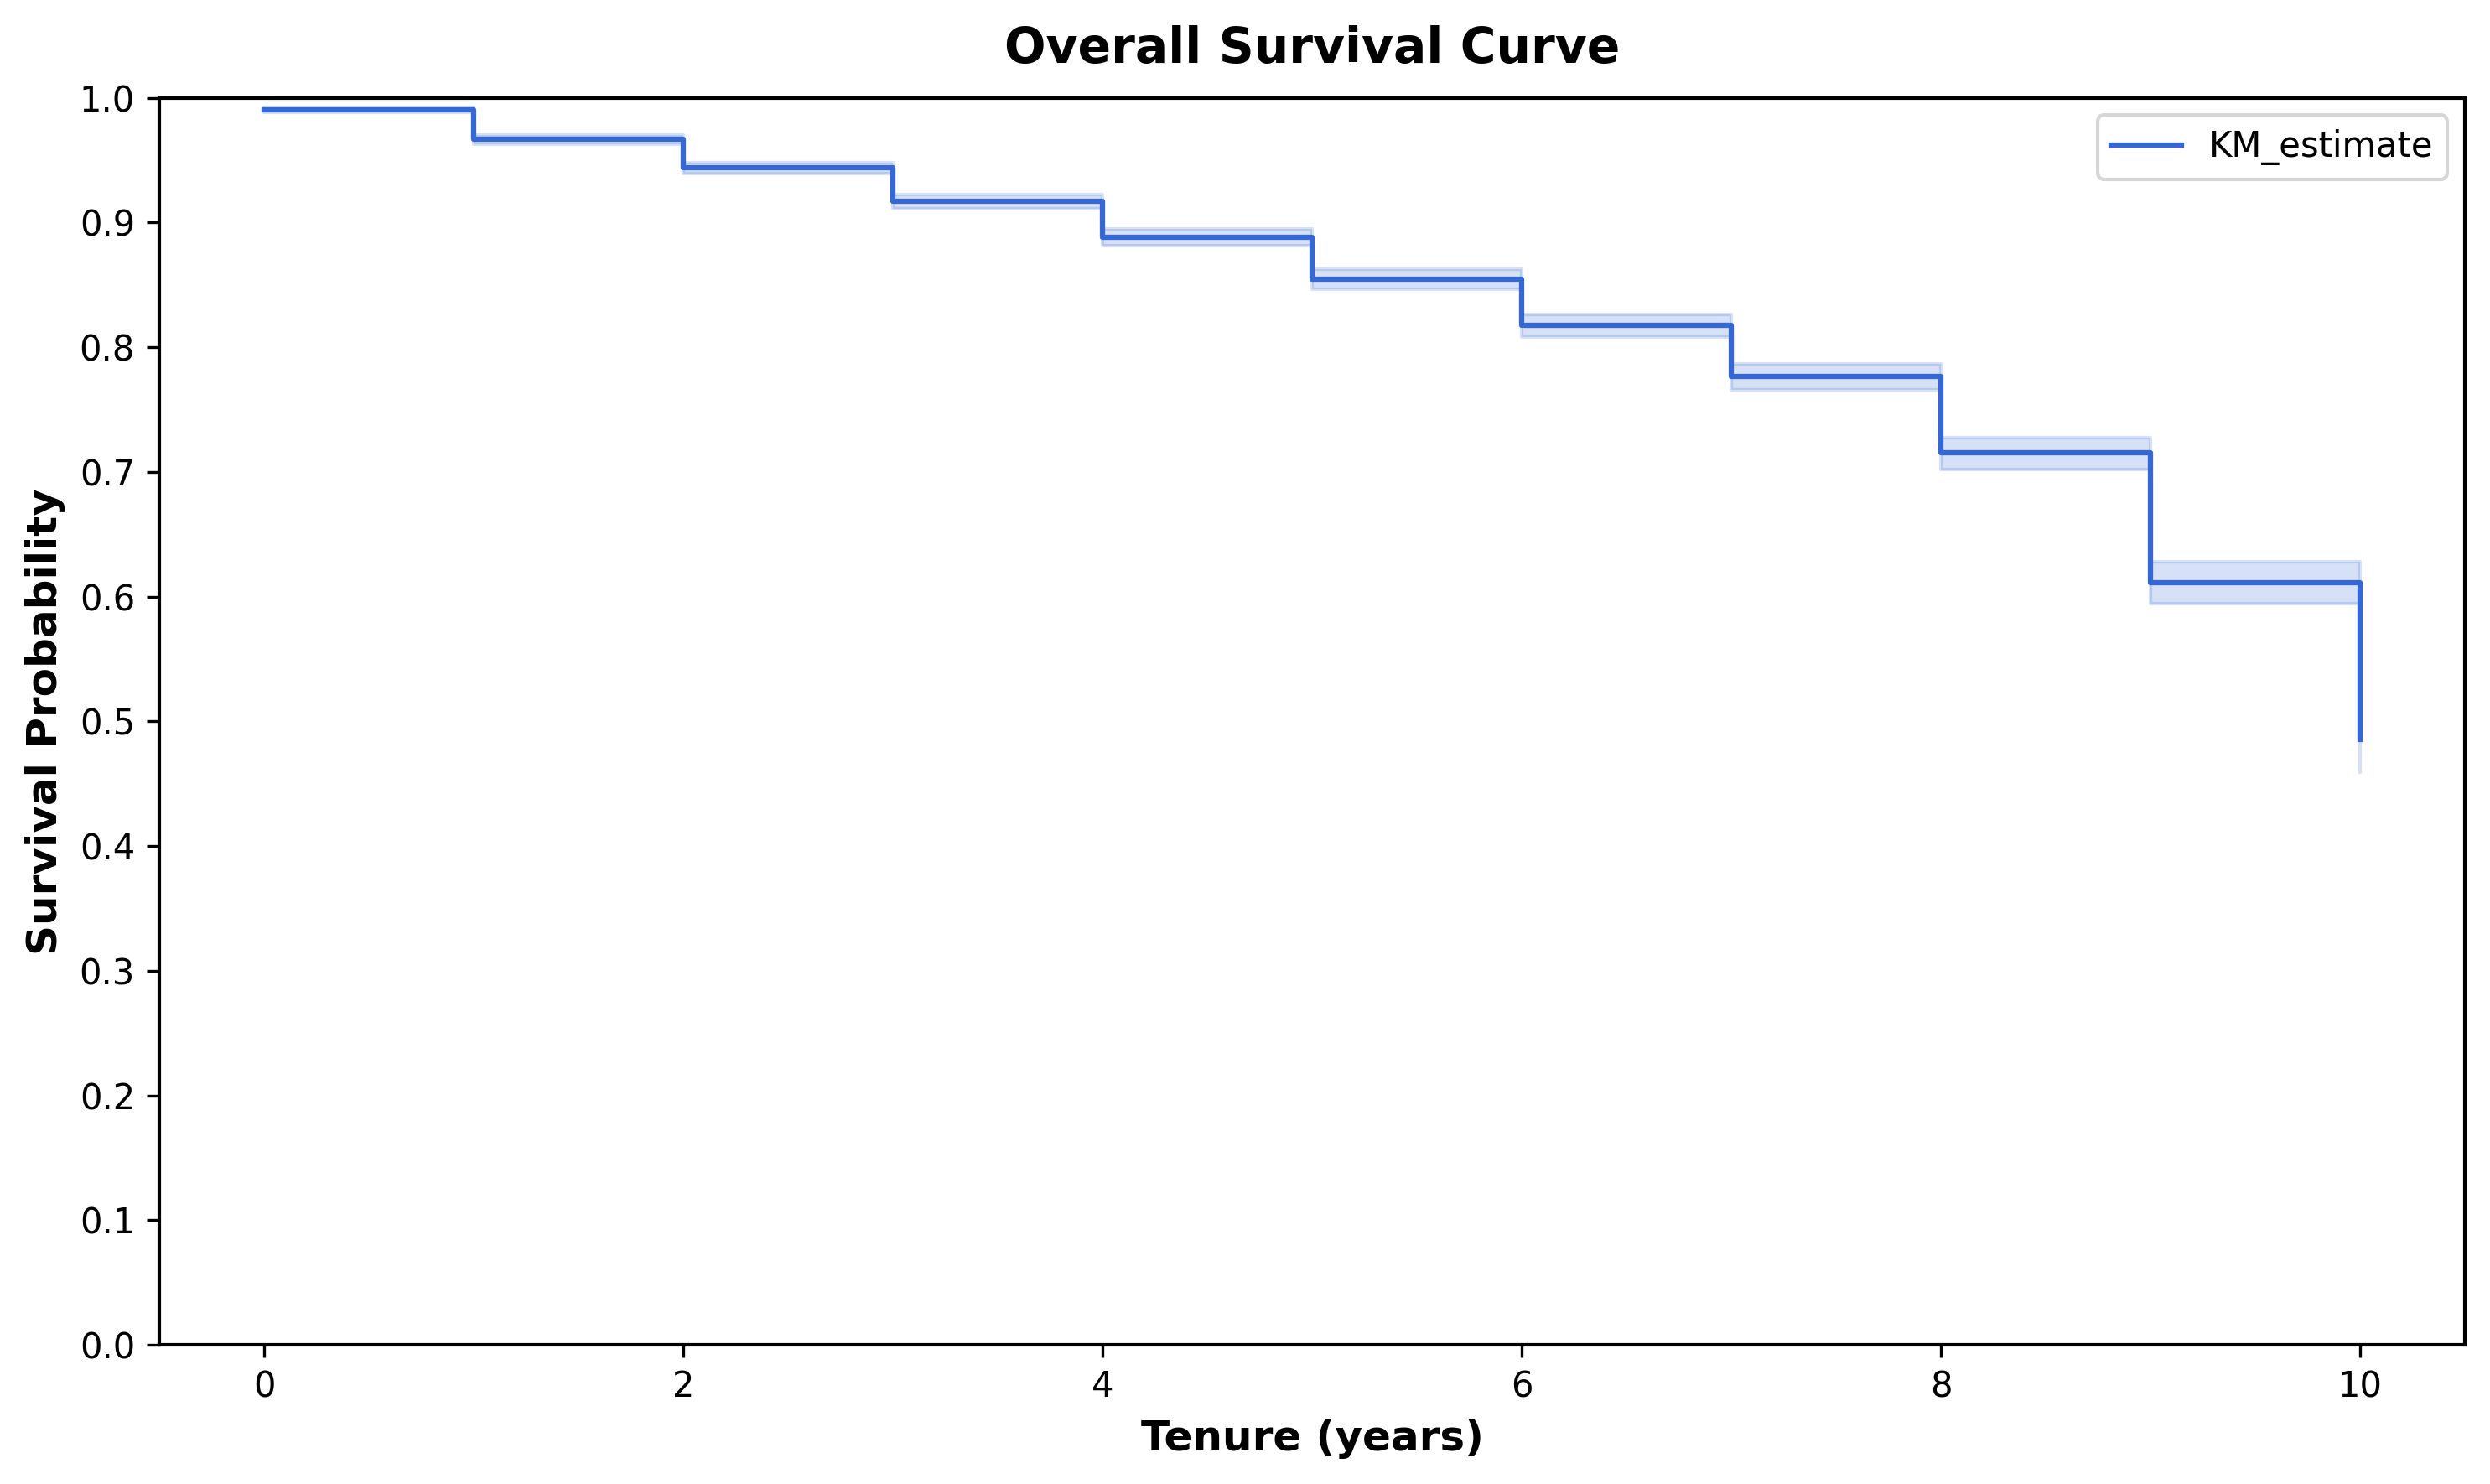
\includegraphics[width=\textwidth]{../img/09_overall_survival_curve_plot.png}
\caption{Overall}
\label{fig:survival_overall}
\end{subfigure}
\hfill
\begin{subfigure}[b]{0.48\textwidth}
\centering
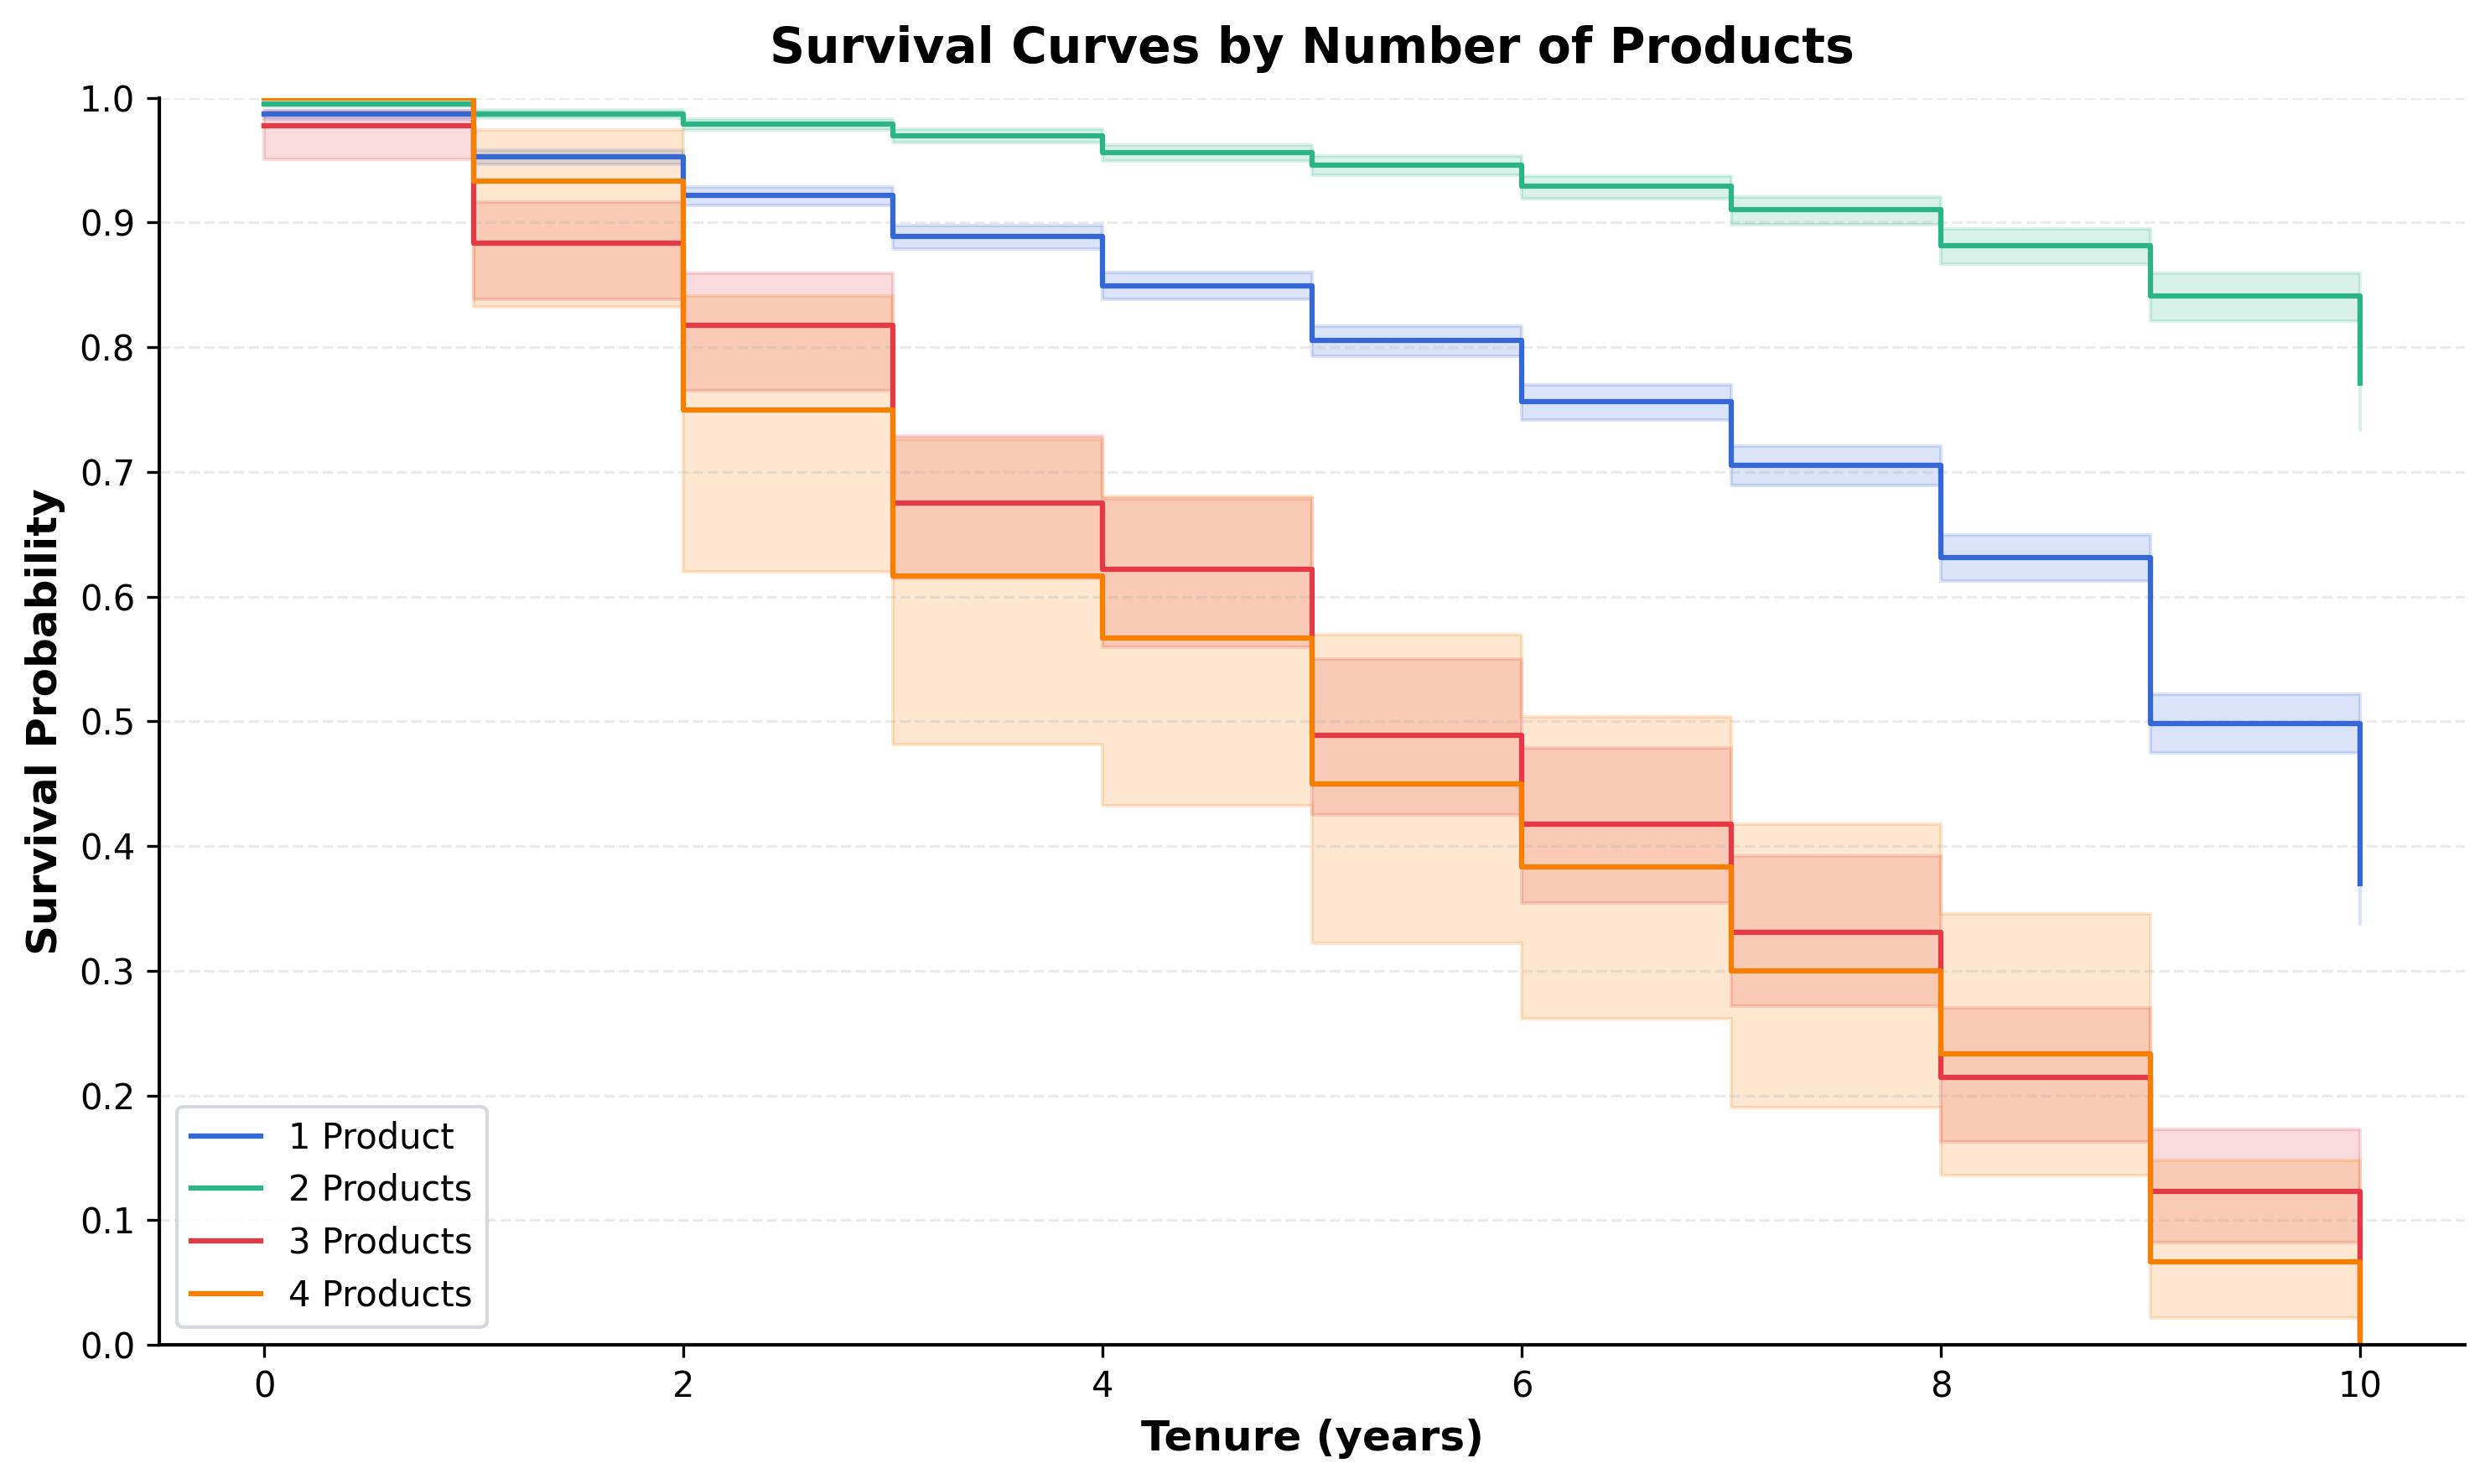
\includegraphics[width=\textwidth]{../img/11_survival_products_plot.png}
\caption{By Product Count}
\label{fig:survival_products}
\end{subfigure}
\vskip\baselineskip
\begin{subfigure}[b]{0.48\textwidth}
\centering
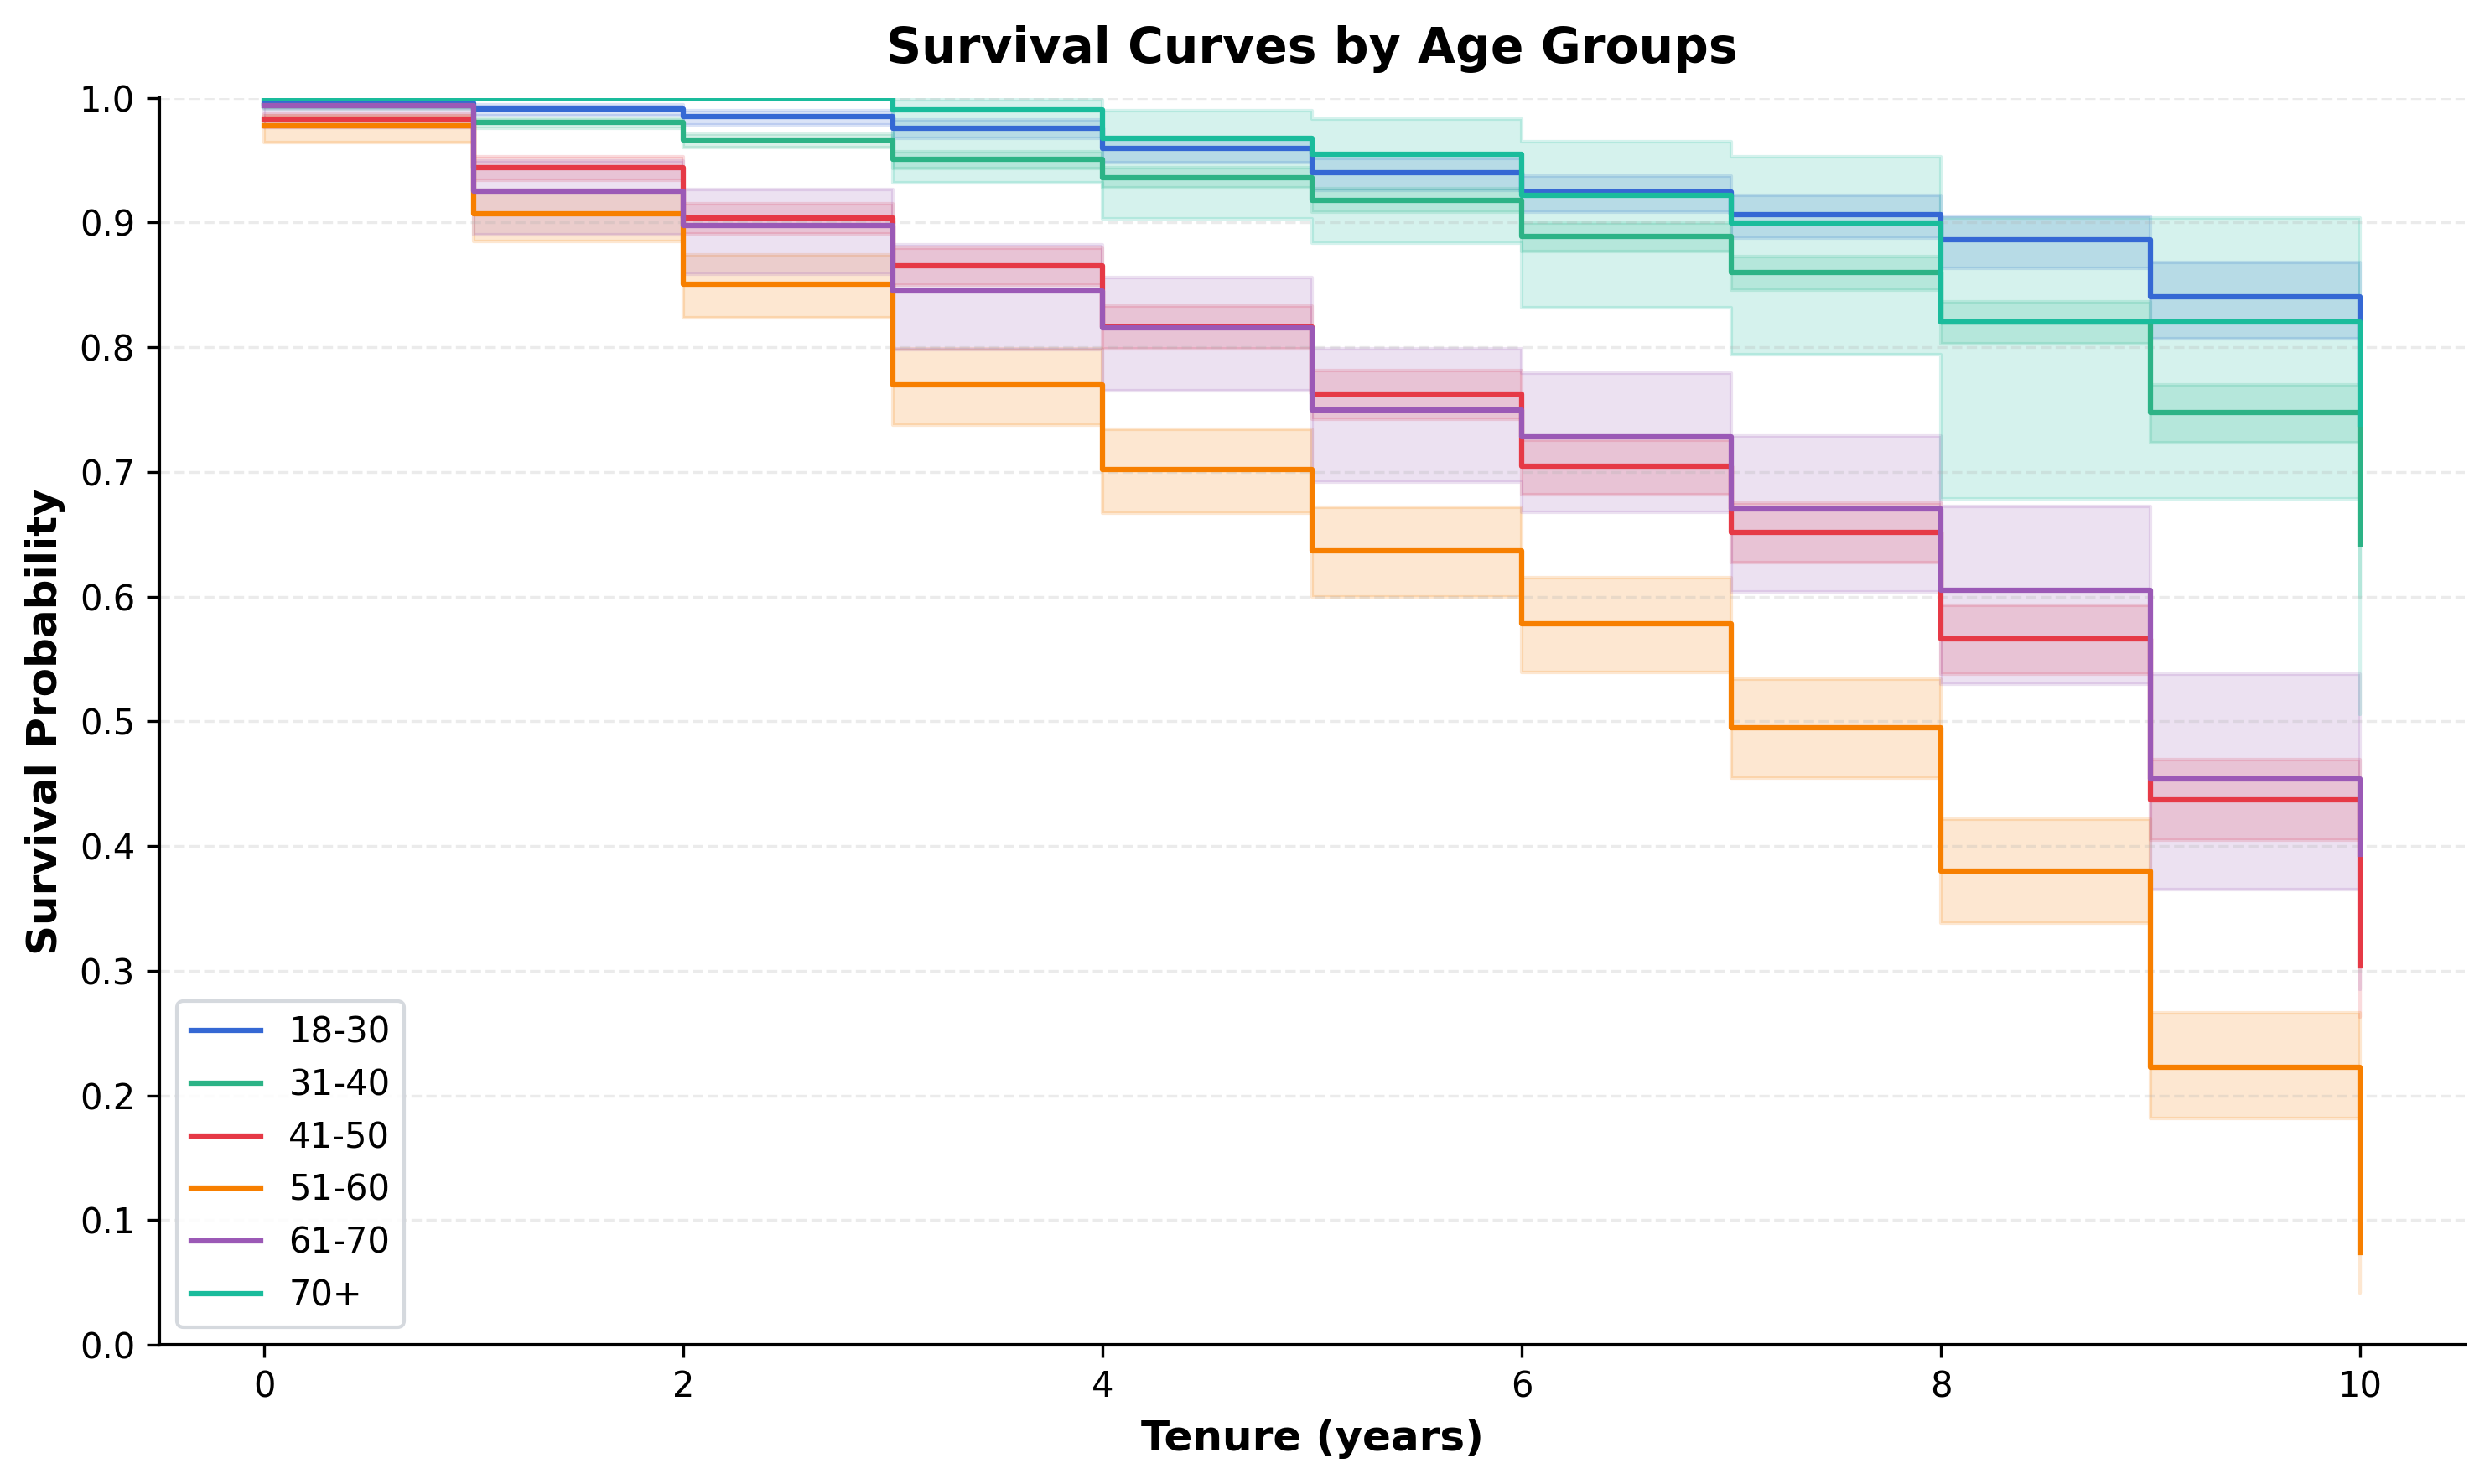
\includegraphics[width=\textwidth]{../img/10_survival_age_groups_plot.png}
\caption{By Age Groups}
\label{fig:survival_age}
\end{subfigure}
\hfill
\begin{subfigure}[b]{0.48\textwidth}
\centering
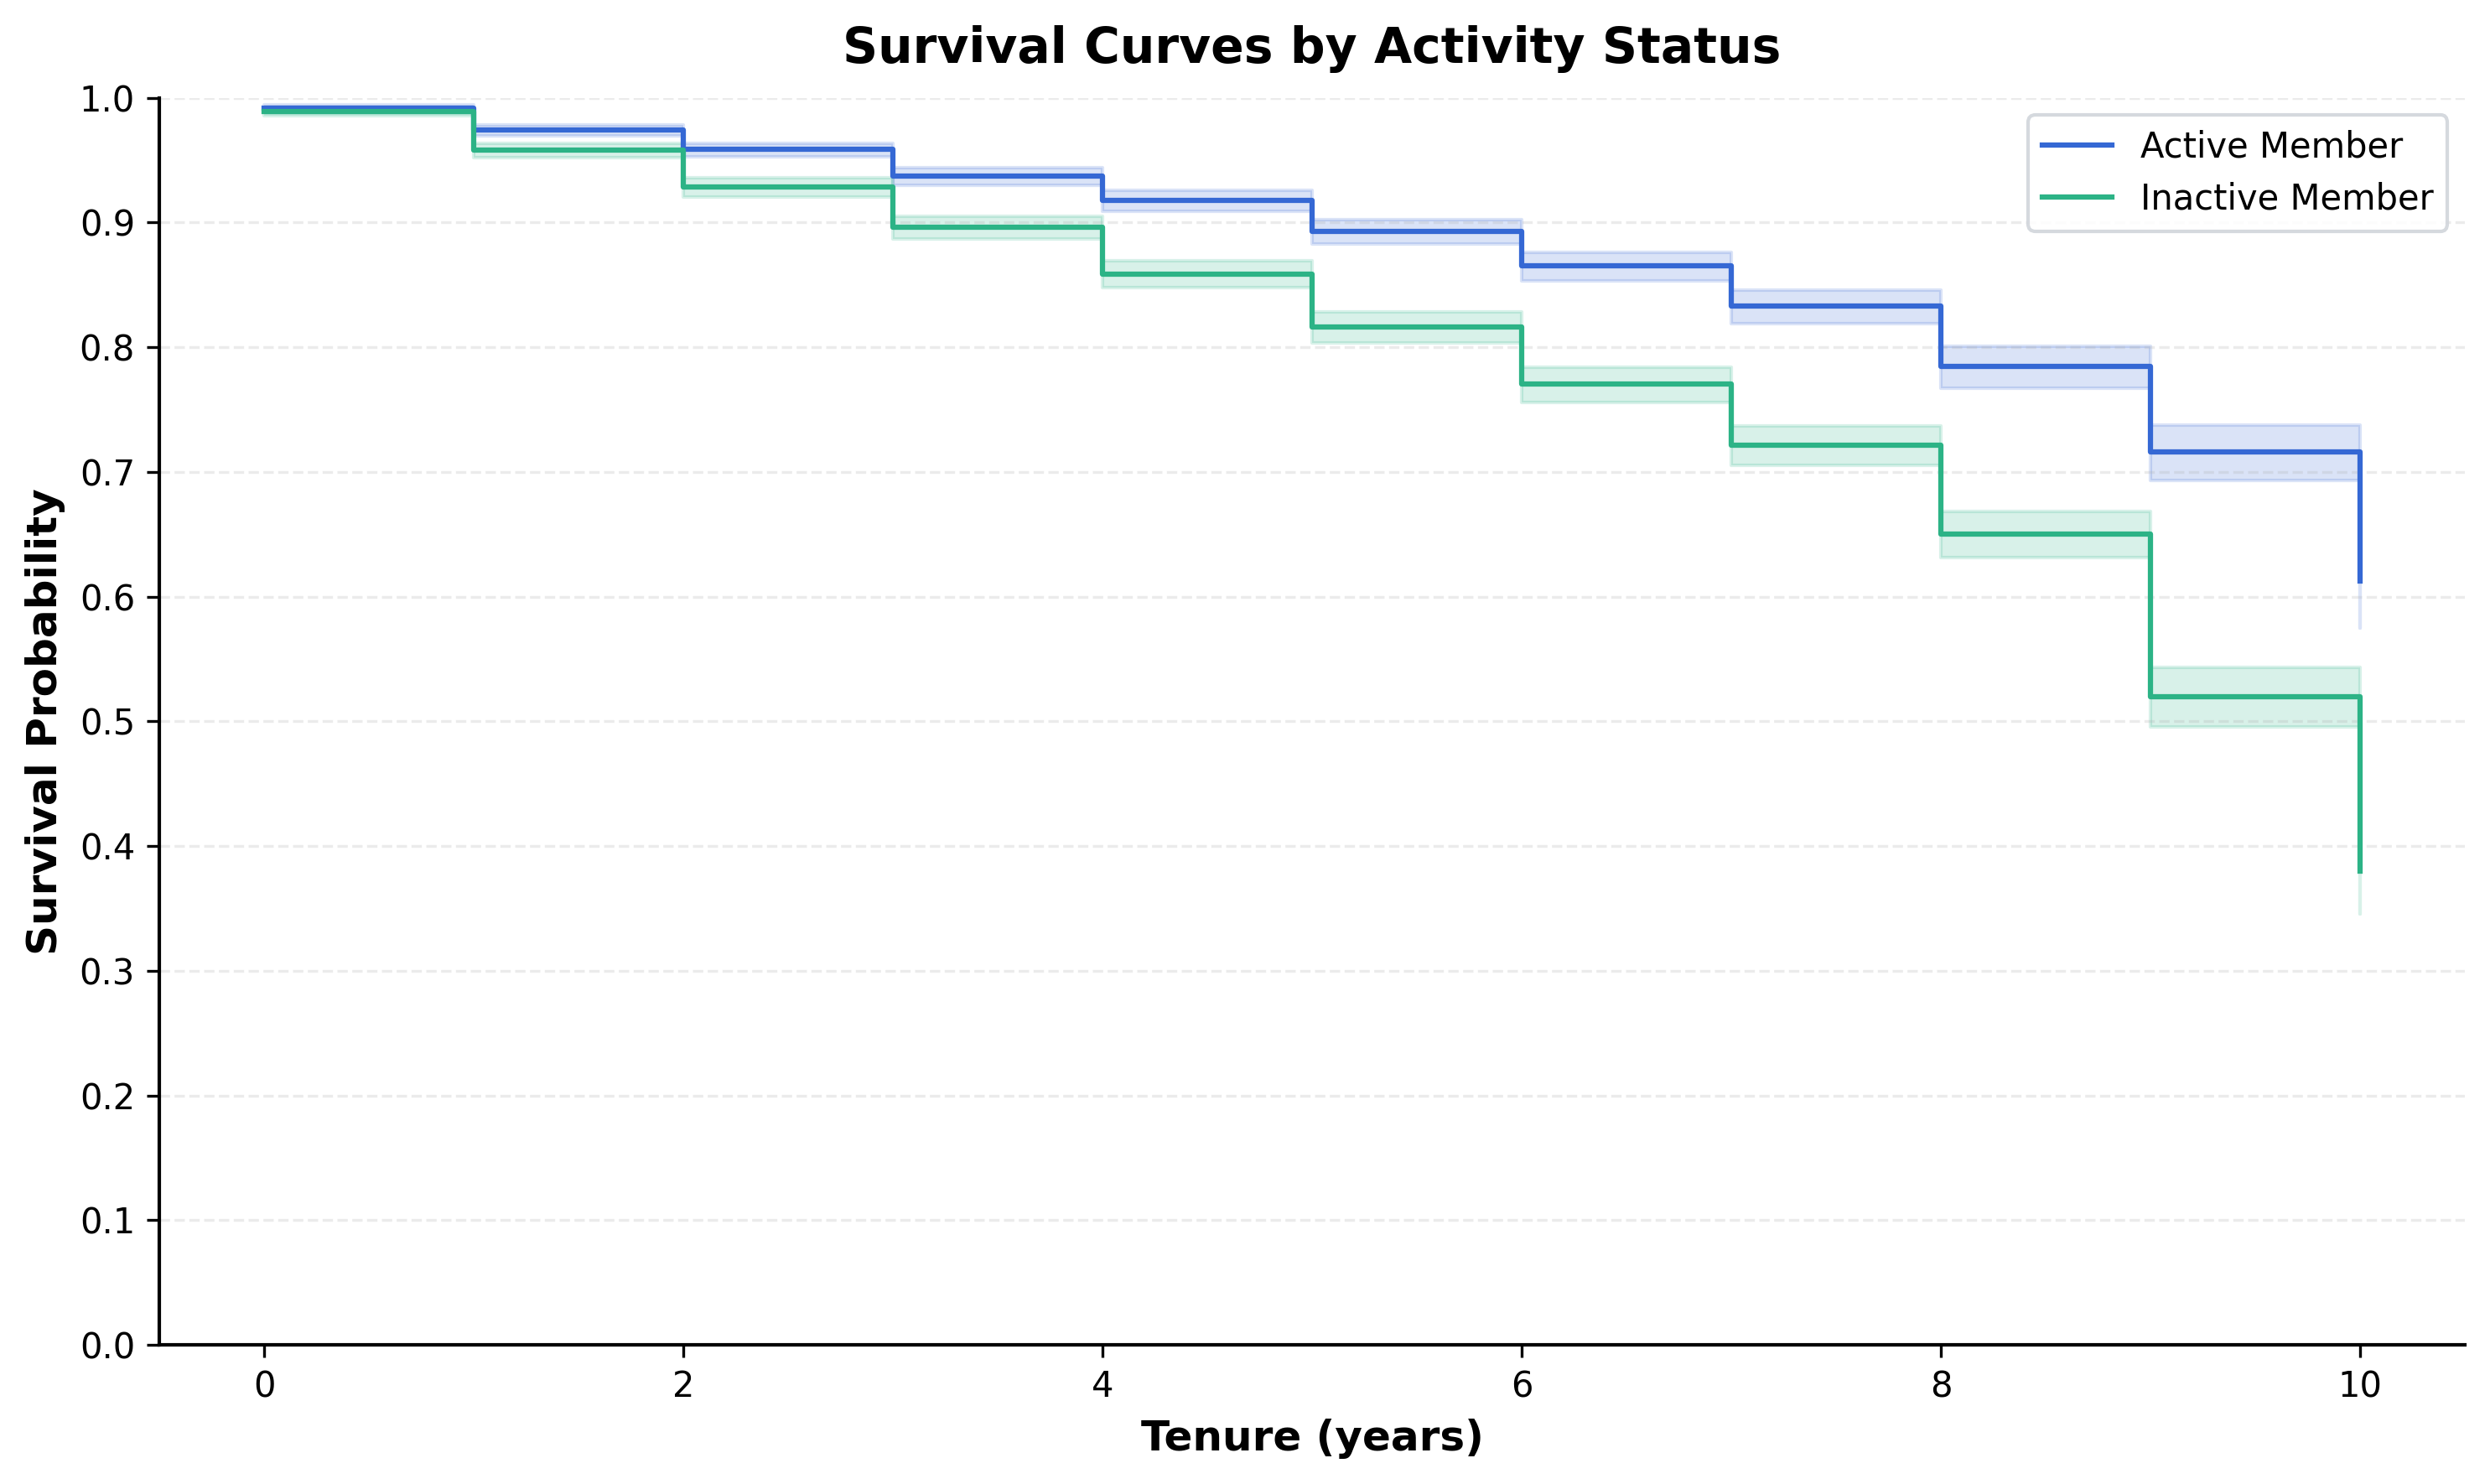
\includegraphics[width=\textwidth]{../img/12_survival_active_status_plot.png}
\caption{By Activity Status}
\label{fig:survival_active}
\end{subfigure}
\caption{Kaplan-Meier survival curves across customer segments. (a) Overall survival exceeds 10 years of tenure for most customers. (b) Product count exhibits U-shaped pattern with 2 products optimal; small sample sizes for 3‑product (n=266) and 4‑product (n=60) groups increase uncertainty. (c) Age groups show peak vulnerability at 51–60 years. (d) Active members maintain higher retention than inactive members. All differences are statistically significant (p $<$ 0.001).}
\label{fig:survival_all}
\end{figure}

Log‑rank tests confirmed that these differences were statistically significant. Table~\ref{tab:logrank_results} summarizes the complete log‑rank test results for all customer segment comparisons, confirming that all features exhibited highly significant differences in survival distributions (p $<$ 0.001).

\begin{table}[H]
\centering
\small
\caption{Log-rank test results comparing survival distributions across customer segments. All features exhibit highly significant differences (p $<$ 0.001).}
\label{tab:logrank_results}
\begin{tabular}{lrr}
\toprule
\textbf{Feature} & \textbf{Test Statistic} & \textbf{p-value} \\
\midrule
Age Group & 1124.09 & $<$ 0.001 \\
Number of Products & 1243.64 & $<$ 0.001 \\
Activity Status & 179.24 & $<$ 0.001 \\
Geography & 243.70 & $<$ 0.001 \\
Gender & 100.47 & $<$ 0.001 \\
Balance Group & 154.37 & $<$ 0.001 \\
\bottomrule
\end{tabular}
\end{table}

The cumulative hazard function \(H(t) = -\ln(S(t))\) provides a complementary perspective to survival curves by quantifying the accumulated risk of churn over time (Figure~\ref{fig:cumulative_hazard}). Churn risk accumulates gradually in the early years but accelerates markedly after approximately 7–8 years of tenure, indicating a critical intervention window.

\begin{figure}[H]
\centering
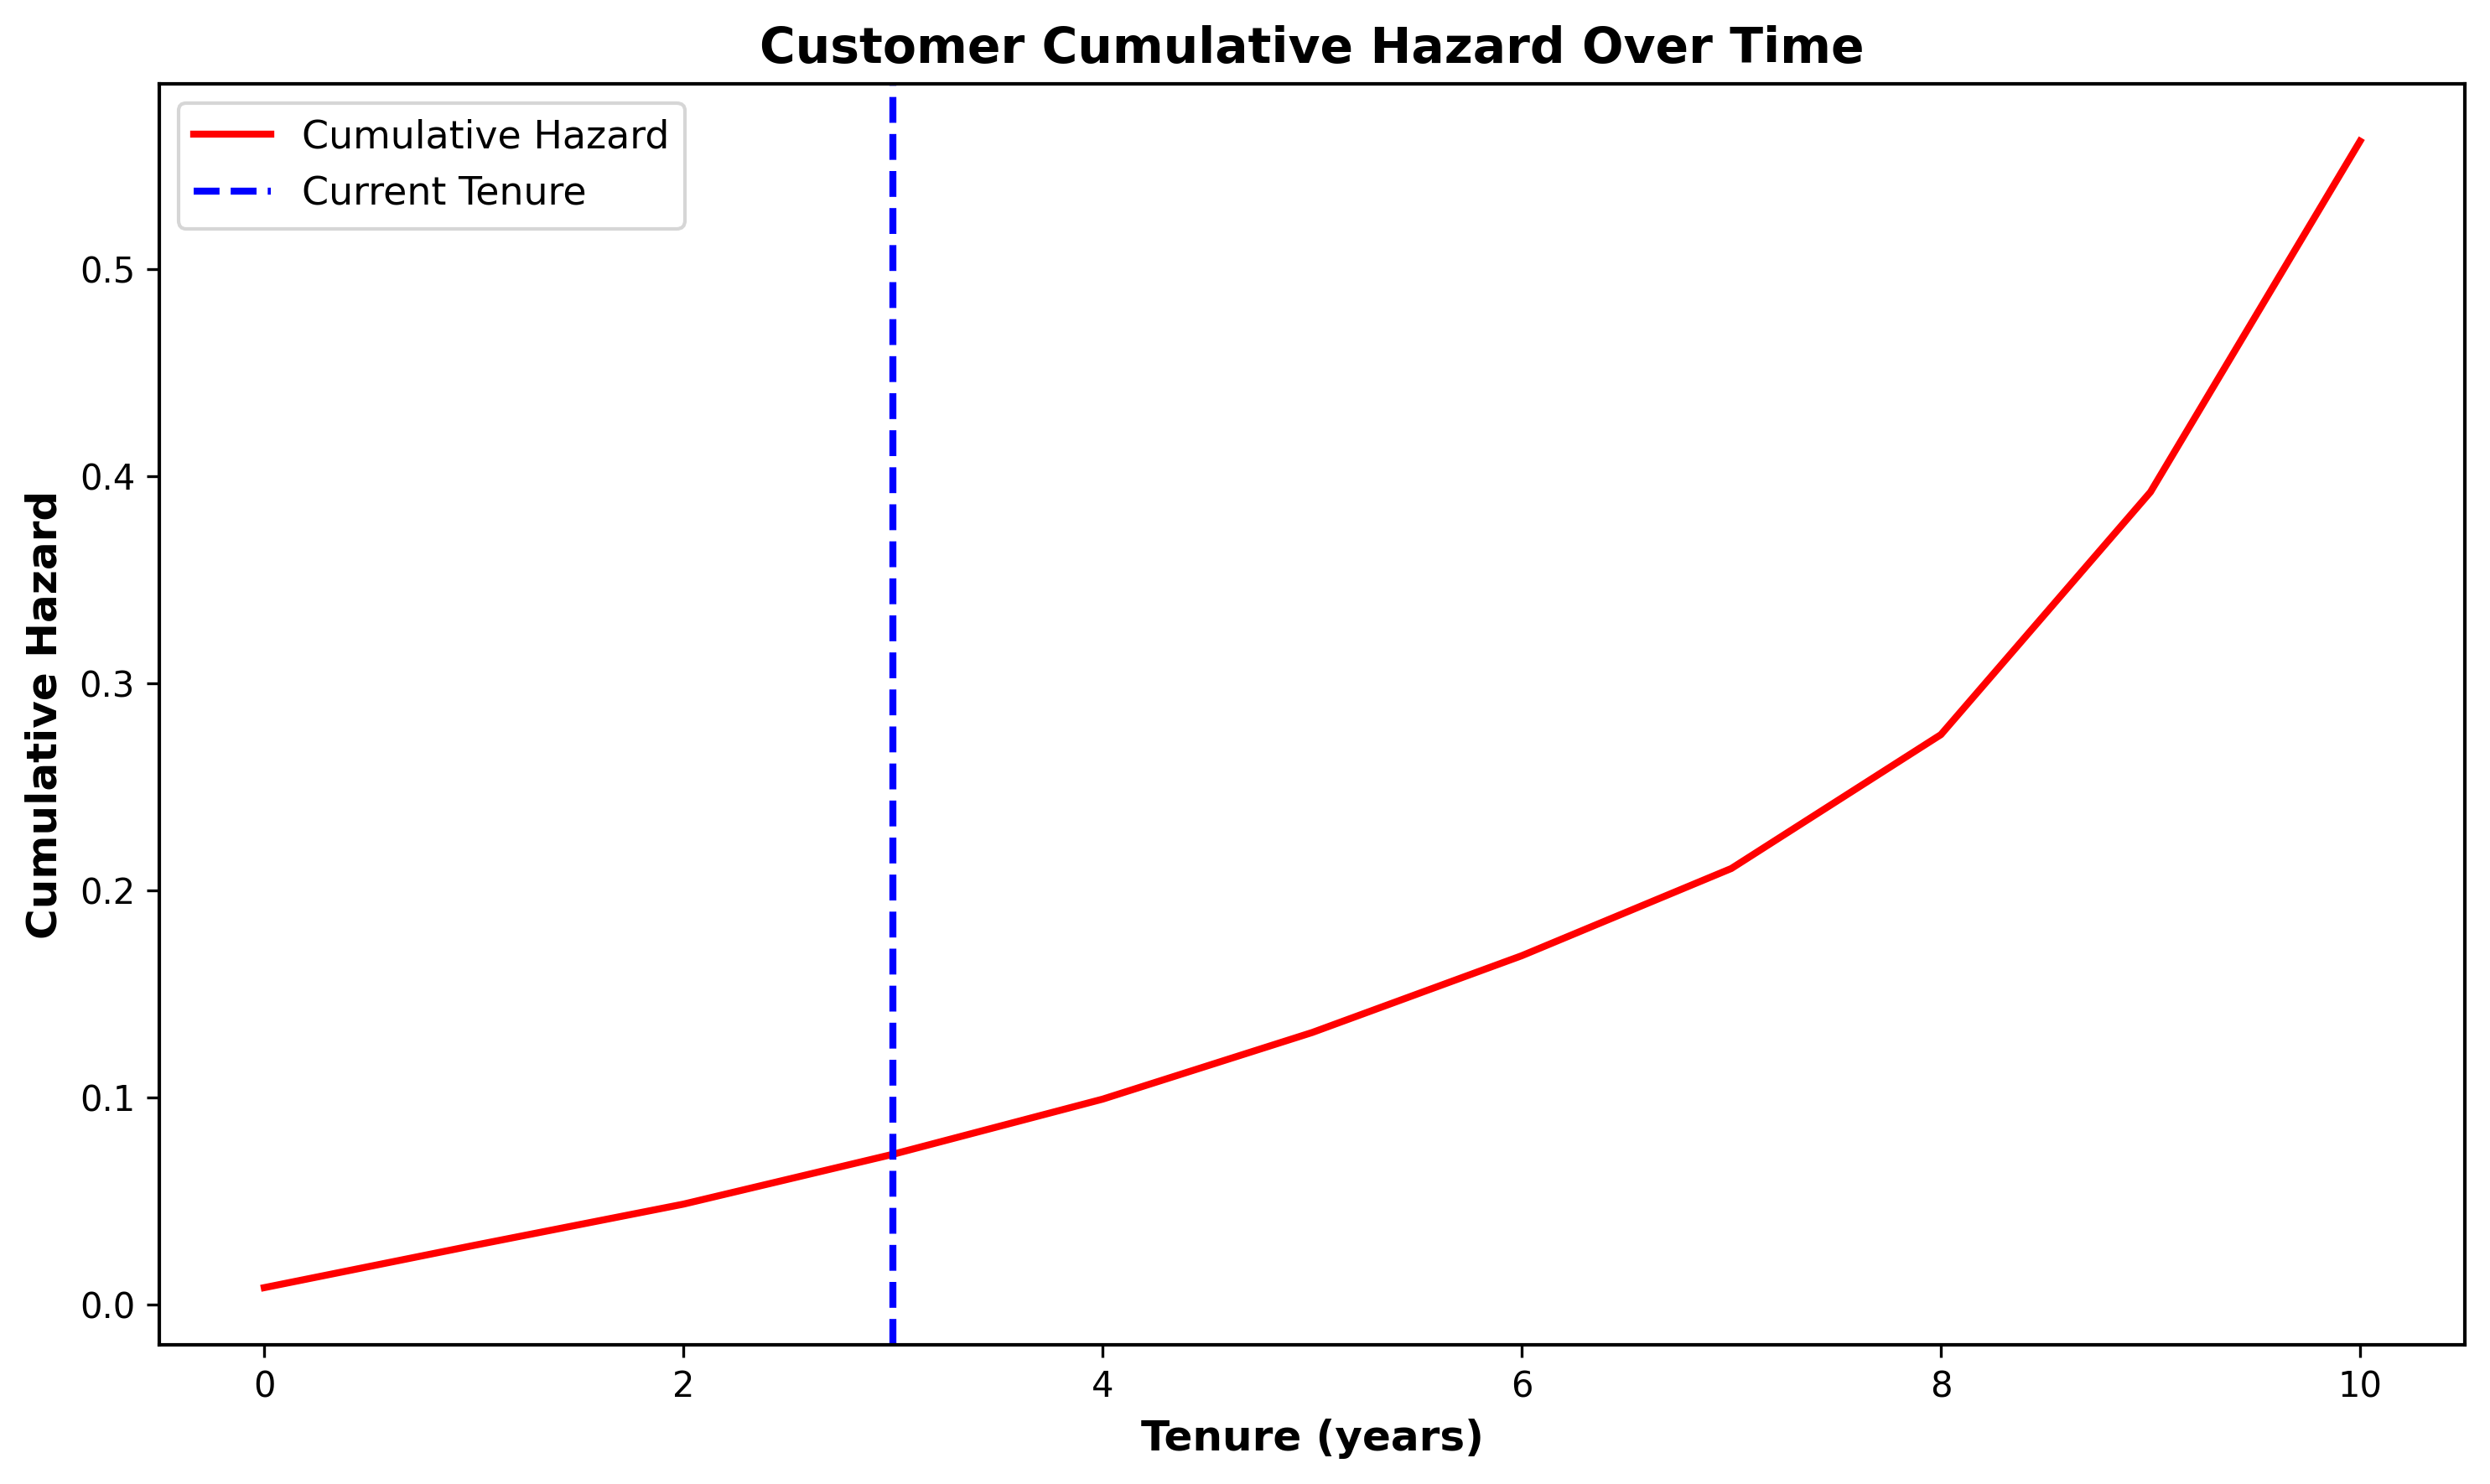
\includegraphics[width=0.7\textwidth]{../img/cumulative_hazard_plot.png}
\caption{Cumulative hazard function for representative customer with 3 years tenure. Accelerating hazard rate after 7–8 years identifies critical intervention window for long‑tenured customers.}
\label{fig:cumulative_hazard}
\end{figure}

\subsubsection{Cox Proportional Hazards Model Results}
The Cox model achieved a concordance index (C‑index) of 0.74, indicating good discriminative power. The proportional hazards assumption was tested using Schoenfeld residuals; all covariates satisfied the assumption (p~$\geq$~0.05 for all time-dependency tests), confirming that hazard ratios remain approximately constant over time and validating the model specification. Hazard ratios quantified the relative risk associated with each feature (Table~\ref{tab:cox_results}). The age 51–60 group had a hazard ratio of 7.94 (95\%~CI [6.59–9.57]), meaning their risk of churn was approximately eight times that of the baseline 18–30 group. Being an active member reduced the hazard by 46~\% (hazard ratio 0.54, 95\%~CI [0.49–0.59]), while German nationality increased the hazard by 60~\% relative to France (HR 1.60, 95\%~CI [1.44–1.78]). The number of products exhibited a linear hazard ratio close to one per additional product (HR=1.02), but this masked the underlying U‑shape seen in the K–M curves.

\begin{table}[H]
\centering
\small
\caption{Cox Proportional Hazards Model Results (excluding complaint status). Concordance Index (C-index): 0.74. Baseline age group: 18-30. Baseline geography: France. HR $>$ 1 indicates increased churn risk; HR $<$ 1 indicates protective effect.}
\label{tab:cox_results}
\begin{tabular}{lccc}
\toprule
\textbf{Feature} & \textbf{Hazard Ratio} & \textbf{95\% CI} & \textbf{p-value} \\
\midrule
\textbf{Age Groups (vs. 18-30)} & & & \\
\phantom{---} 31-40 & 1.61 & [1.34–1.93] & $<$0.001 \\
\phantom{---} 41-50 & 4.31 & [3.61–5.14] & $<$0.001 \\
\phantom{---} 51-60 & 7.94 & [6.59–9.57] & $<$0.001 \\
\phantom{---} 61-70 & 5.12 & [3.98–6.59] & $<$0.001 \\
\phantom{---} 70+ & 1.30 & [0.71–2.41] & 0.378 \\
\midrule
\textbf{Other Features} & & & \\
\phantom{---} Gender (Female) & 1.47 & [1.34–1.60] & $<$0.001 \\
\phantom{---} IsActiveMember & 0.54 & [0.49–0.59] & $<$0.001 \\
\phantom{---} Geography (Germany) & 1.60 & [1.44–1.78] & $<$0.001 \\
\phantom{---} Geography (Spain) & 1.05 & [0.94–1.19] & 0.379 \\
\phantom{---} NumOfProducts & 0.92 & [0.86–0.99] & 0.035 \\
\phantom{---} Balance & 1.00 & [1.00–1.00] & $<$0.001 \\
\phantom{---} Tenure & 0.99 & [0.97–1.00] & 0.156 \\
\bottomrule
\end{tabular}
\end{table}

\begin{figure}[H]
\centering
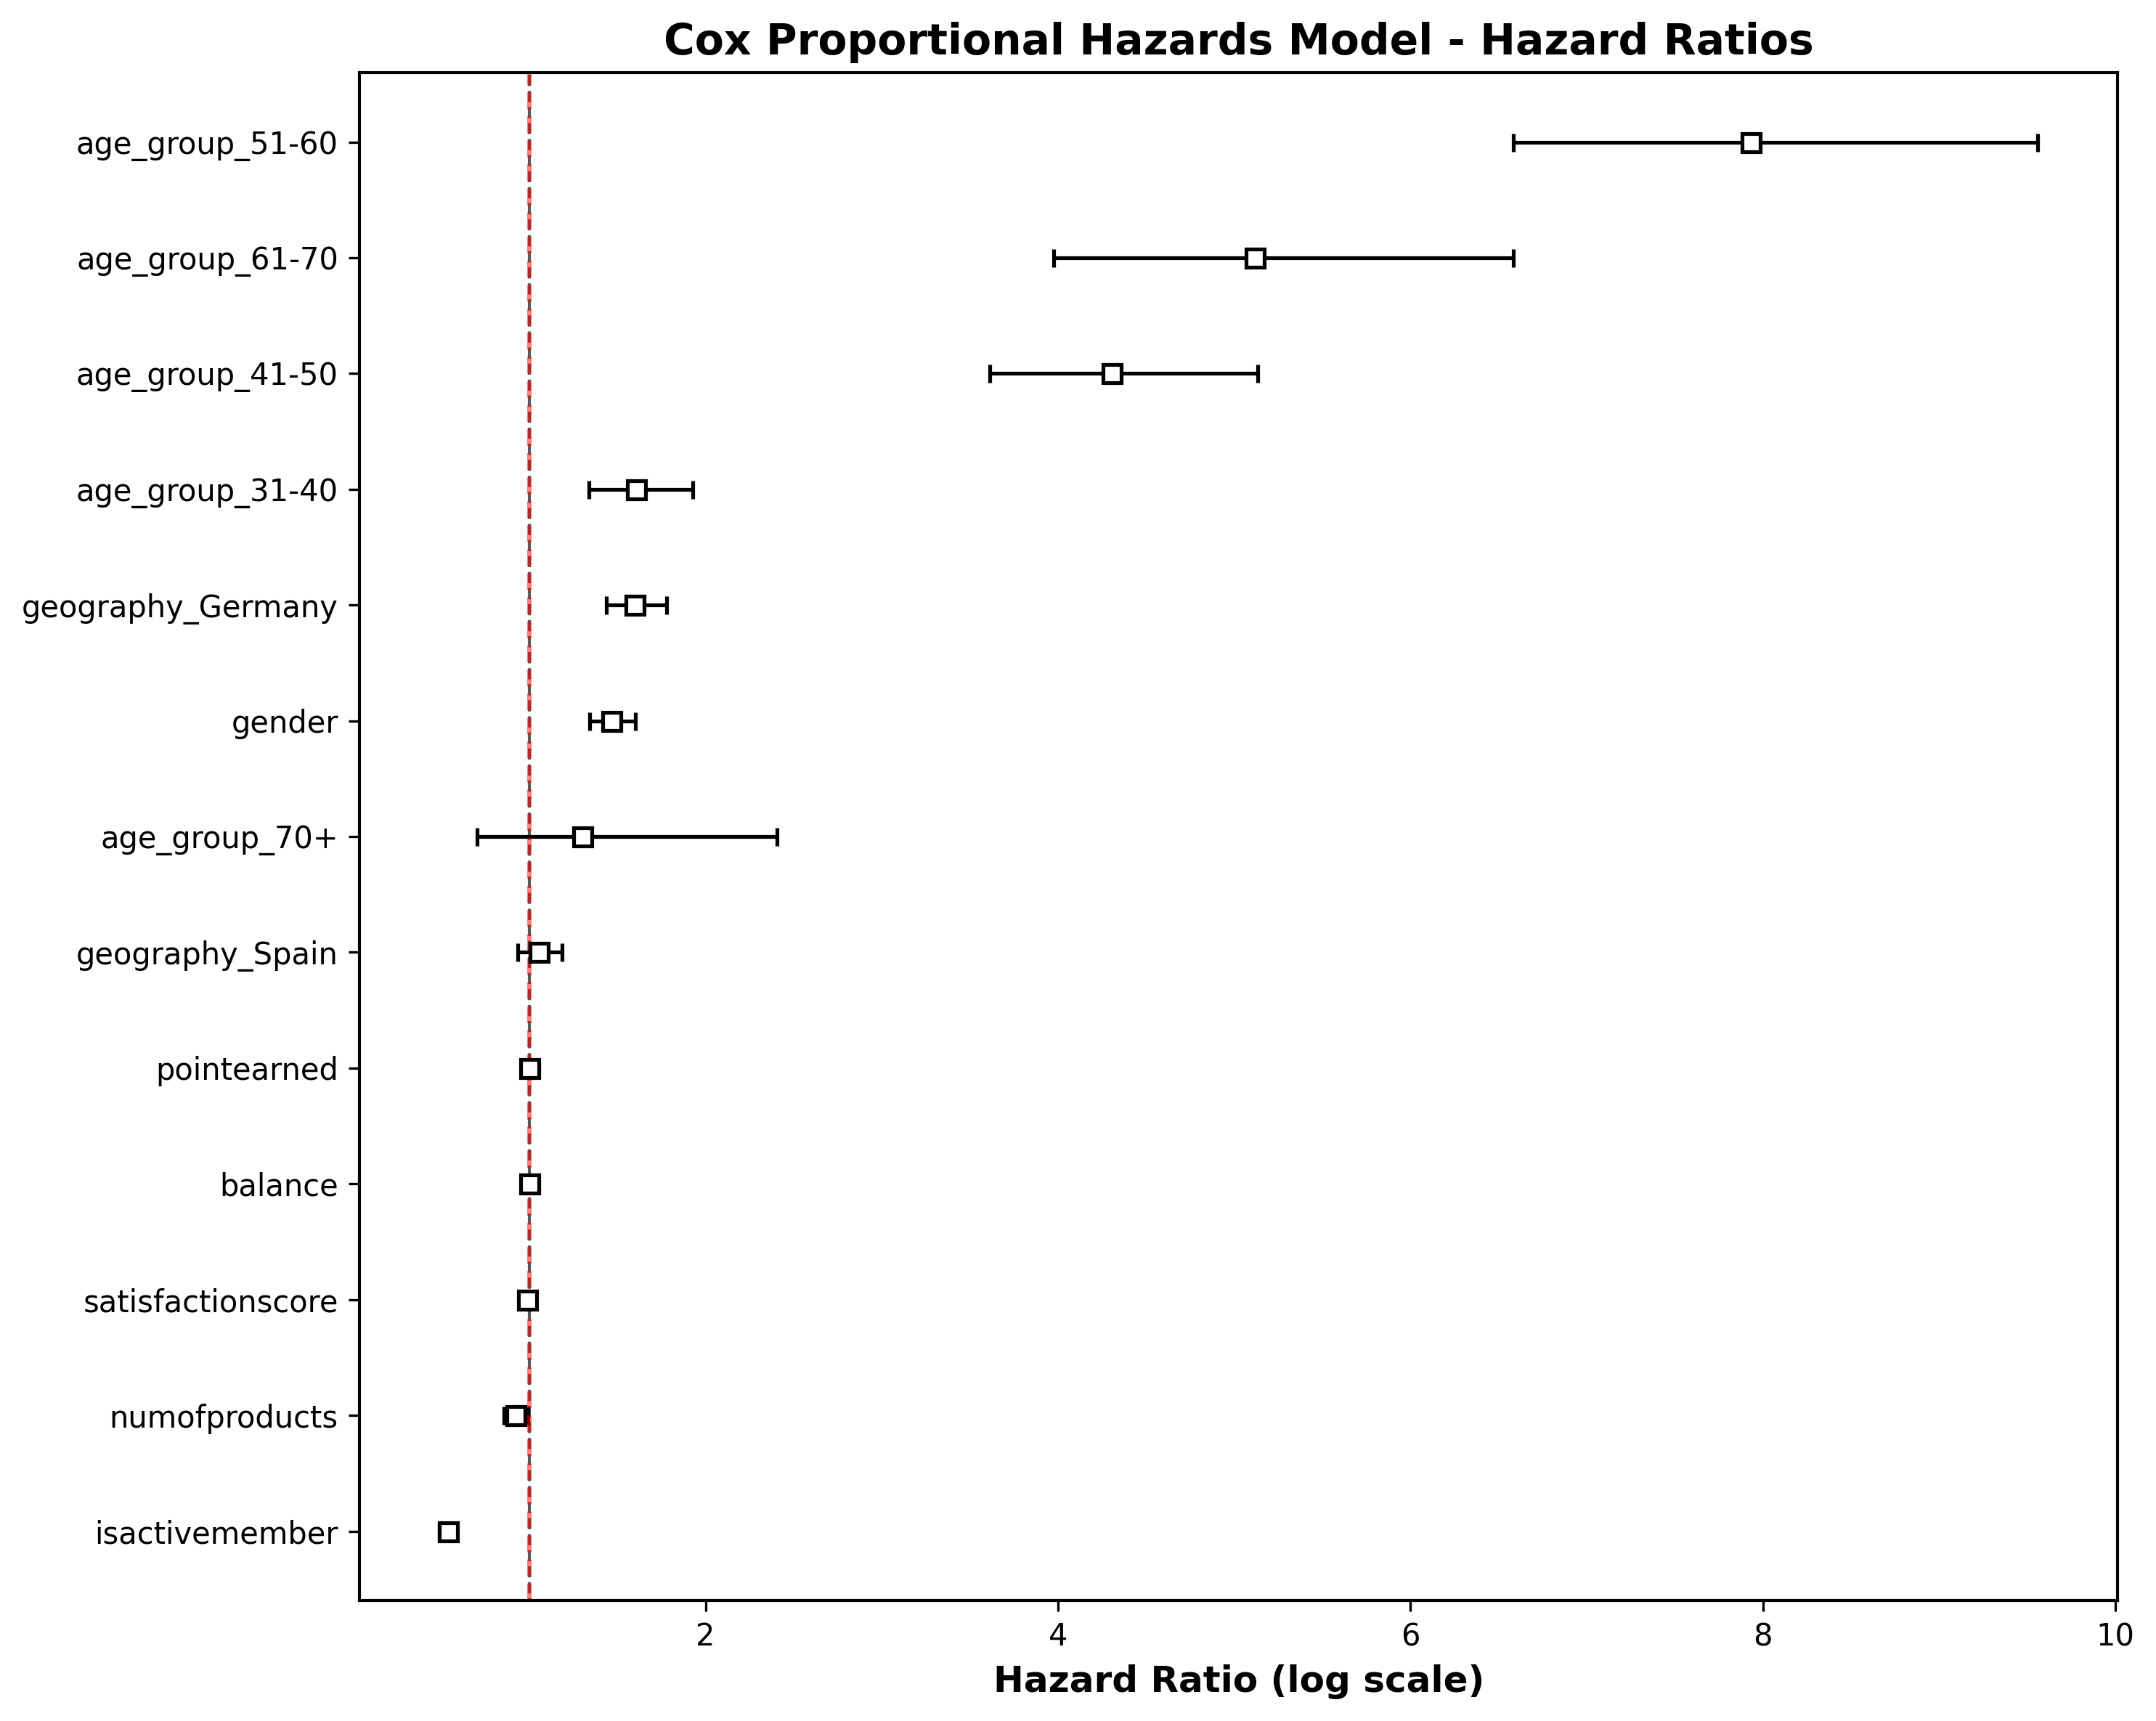
\includegraphics[width=0.7\textwidth]{../img/14_cox_ph_coefficients.png}
\caption{Cox Proportional Hazards model coefficients. Hazard ratios quantify relative churn risk for each feature.}
\label{fig:cox_coefficients}
\end{figure}

\subsection{Predictive Model Performance}
A random forest classifier was developed to identify at-risk customers before explicit signals of dissatisfaction emerge. The model provides probabilistic risk scores that enable proactive intervention, complementing the temporal insights from survival analysis with actionable predictive intelligence.

The four-stage grid search identified an optimal Random Forest configuration consisting of 900 trees, maximum depth of 11, Gini impurity criterion, no feature subsetting (max\_features=None), minimum split size of four samples, and class weight ratio \(\{0:1,1:2\}\). Cross-validation on the training set yielded mean F1-score of 59.6\% (standard deviation: 1.8\%), indicating stable performance across different data splits and supporting claims of generalization capability.

On the 2,000-sample test set, the model achieved 57.8\% recall, representing a 21 percentage point improvement over the untuned baseline and correctly identifying 236 of 408 churners before they exit. Overall accuracy of 85.9\% represents a 6.3 percentage point improvement over the majority-class baseline (79.6\%). Class-specific performance metrics (Table~\ref{tab:model_performance}) showed precision of 68.0\%, recall of 57.8\% and F1‑score of 62.5\%. The recall improvement is particularly critical for churn prediction, where failing to identify at-risk customers (false negatives) represents substantially higher cost than false positive retention campaign costs. The model's 57.8\% recall means 172 churners were missed; however, the 68.0\% precision ensures that retention efforts target genuinely at-risk customers with reasonable efficiency.

\begin{table}[H]
\centering
\small
\caption{Model performance metrics summary. Test set contains 2,000 samples with 20.4\% churn rate. Model correctly identified 236 of 408 churners (57.8\% recall).}
\label{tab:model_performance}
\begin{tabular}{lcp{9.5cm}}
\toprule
\textbf{Metric} & \textbf{Value} & \textbf{Interpretation} \\
\midrule
Accuracy & 85.9\% & Share of decisions correct; sensitive to class imbalance. \\
\cmidrule(lr){1-3}
Precision & 68.0\% & Fraction of flagged churners that actually churn; drives retention efficiency. \\
\cmidrule(lr){1-3}
Recall & 57.8\% & Fraction of actual churners caught; primary lever for reducing missed churn. \\
\cmidrule(lr){1-3}
F1-Score & 62.5\% & Balance of precision/recall; single-number summary under asymmetric costs. \\
\cmidrule(lr){1-3}
ROC-AUC & 0.858 & Probability model ranks churner above non-churner; threshold-agnostic. \\
\cmidrule(lr){1-3}
PR-AUC & 0.712 & Average precision across recalls; more informative under class imbalance. \\
\bottomrule
\end{tabular}
\end{table}

Receiver‑operating characteristic (ROC) curves yielded an area under the curve (AUC) of 0.858, indicating strong threshold-agnostic discrimination between churners and non‑churners. The classifier achieves a lower PR-AUC of 0.712 compared to ROC-AUC, reflecting the inherent challenge of maintaining high precision under class imbalance (20.4~\% churn rate). Note that these AUC values are reported on the holdout test set; bootstrap confidence intervals would typically range from approximately 0.83–0.89 for ROC-AUC given a test sample size of 2,000. The confusion matrix (Table~\ref{tab:confusion_matrix}) shows the model correctly identified 236 of 408 churners at the chosen decision threshold; 172 churners were missed, while 111 non-churners were incorrectly flagged as churn risks.

\begin{table}[H]
\centering
\small
\caption{Confusion matrix showing model predictions versus actual outcomes. Model correctly identified 236 churners while missing 172.}
\label{tab:confusion_matrix}
\begin{tabular}{lcc}
\toprule
& \textbf{Predicted: Retained} & \textbf{Predicted: Churned} \\
\midrule
\textbf{Actual: Retained} & 1,481 (TN) & 111 (FP) \\
\textbf{Actual: Churned} & 172 (FN) & 236 (TP) \\
\bottomrule
\end{tabular}
\end{table}

\begin{figure}[H]
\centering
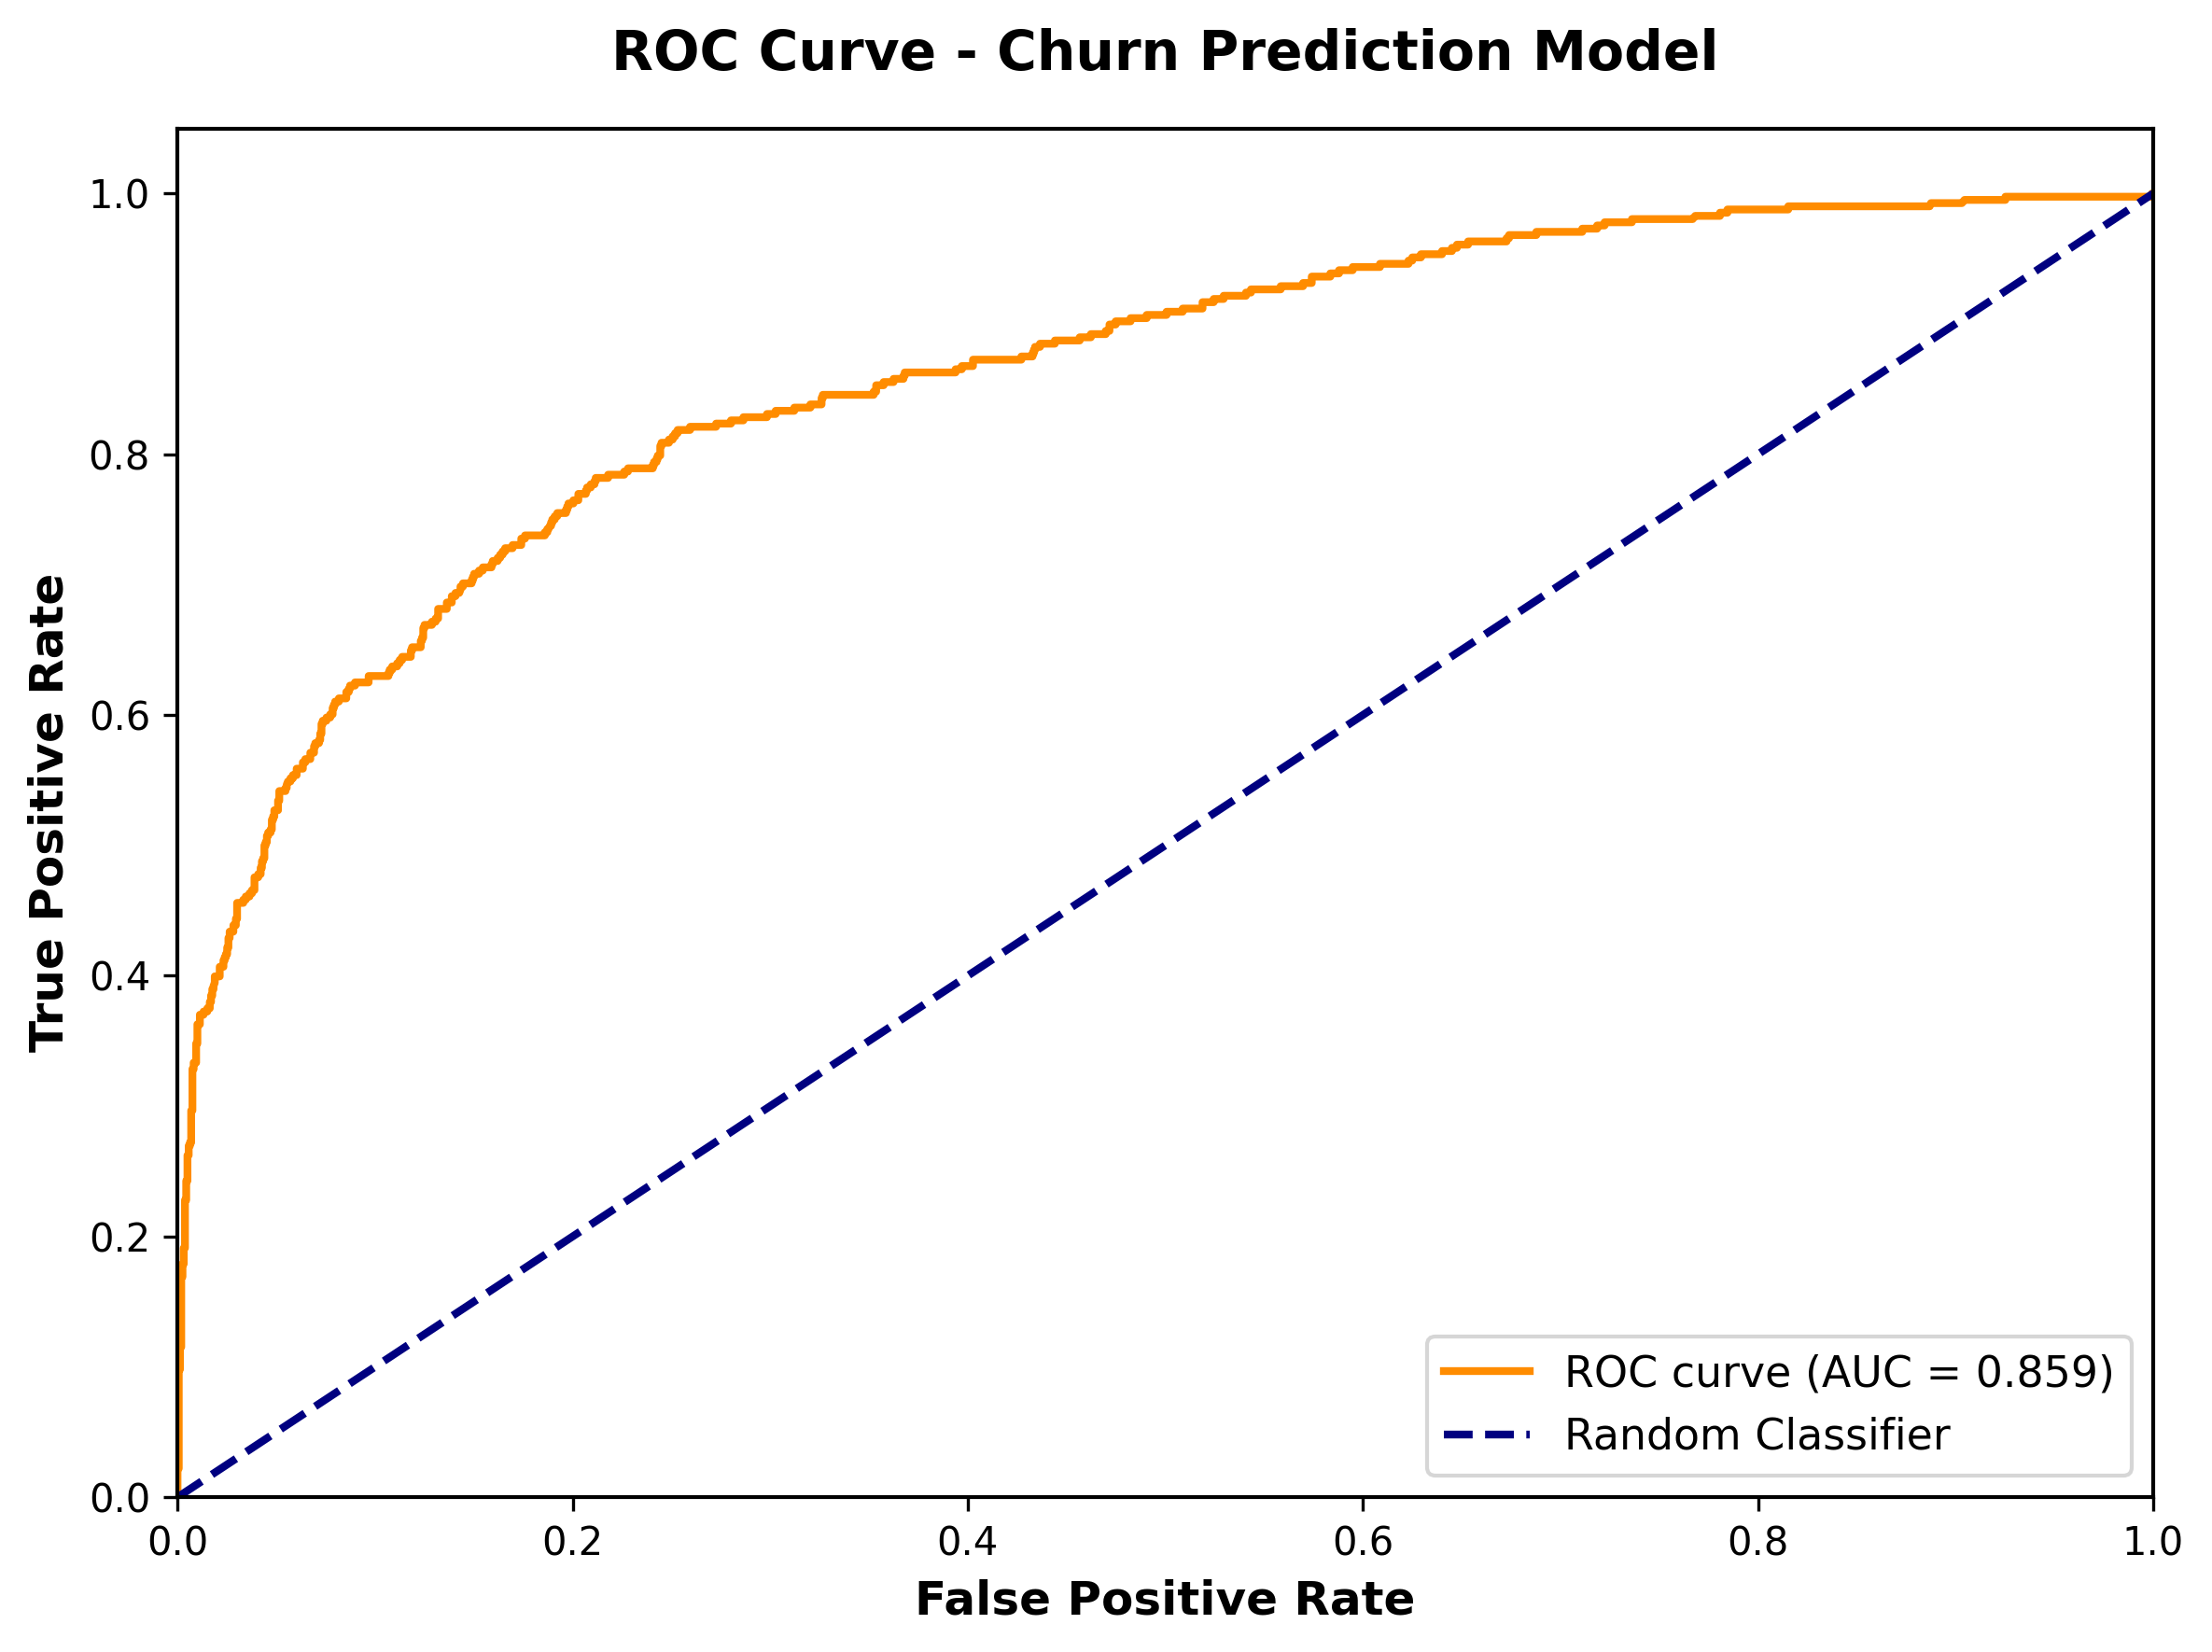
\includegraphics[width=0.6\textwidth]{../img/17_roc_curve.png}
\caption{ROC curve demonstrating model discriminative power. Area under curve (AUC) equals 0.858.}
\label{fig:roc_curve}
\end{figure}

The ROC-AUC quantifies the probability that the classifier ranks a randomly chosen positive instance higher than a randomly chosen negative instance, while PR-AUC measures average precision across all recall thresholds.

Feature importance was assessed using built‑in impurity measures, permutation importance and SHAP (Shapley Additive Explanations) values (Figure~\ref{fig:feature_importance}). Permutation importance measures the decrease in model performance when a feature is randomly shuffled:
\[ I_j = \mathbb{E}[L(y, f(\mathbf{x}_{\text{perm}(j)}))] - \mathbb{E}[L(y, f(\mathbf{x}))], \]
where \(\mathbf{x}_{\text{perm}(j)}\) denotes the feature vector with the \(j\)-th feature randomly permuted, and \(L\) is the loss function. SHAP values provide a unified framework for feature attribution based on Shapley values from cooperative game theory, quantifying each feature's marginal contribution to individual predictions.

Mean absolute SHAP values across all test predictions (Table~\ref{tab:shap_importance}) provide quantitative ranking of feature importance. Age emerged as the most influential predictor (mean absolute SHAP = 0.140), followed by number of products (0.113) and activity status (0.082). Activity status, balance and German nationality were important but secondary drivers.

\begin{table}[H]
\centering
\small
\caption{Mean absolute SHAP values quantifying feature importance. Higher values indicate greater average impact on predictions across all customers.}
\label{tab:shap_importance}
\begin{tabular}{lcc}
\toprule
\textbf{Feature} & \textbf{Mean Absolute SHAP} & \textbf{Rank} \\
\midrule
Age & 0.140 & 1 \\
NumOfProducts & 0.113 & 2 \\
IsActiveMember & 0.082 & 3 \\
Balance & 0.041 & 4 \\
Geography\_Germany & 0.027 & 5 \\
Gender & 0.020 & 6 \\
Geography\_Spain & 0.009 & 7 \\
Tenure & 0.007 & 8 \\
\bottomrule
\end{tabular}
\end{table}

Partial dependence analysis (Figure~\ref{fig:pdp_age}) confirmed the near‑monotonic increase in churn probability with age up to the 51–60 group, while exploratory data analysis (Section 2) revealed the U‑shaped effect of the number of products.

\begin{figure}[H]
\centering
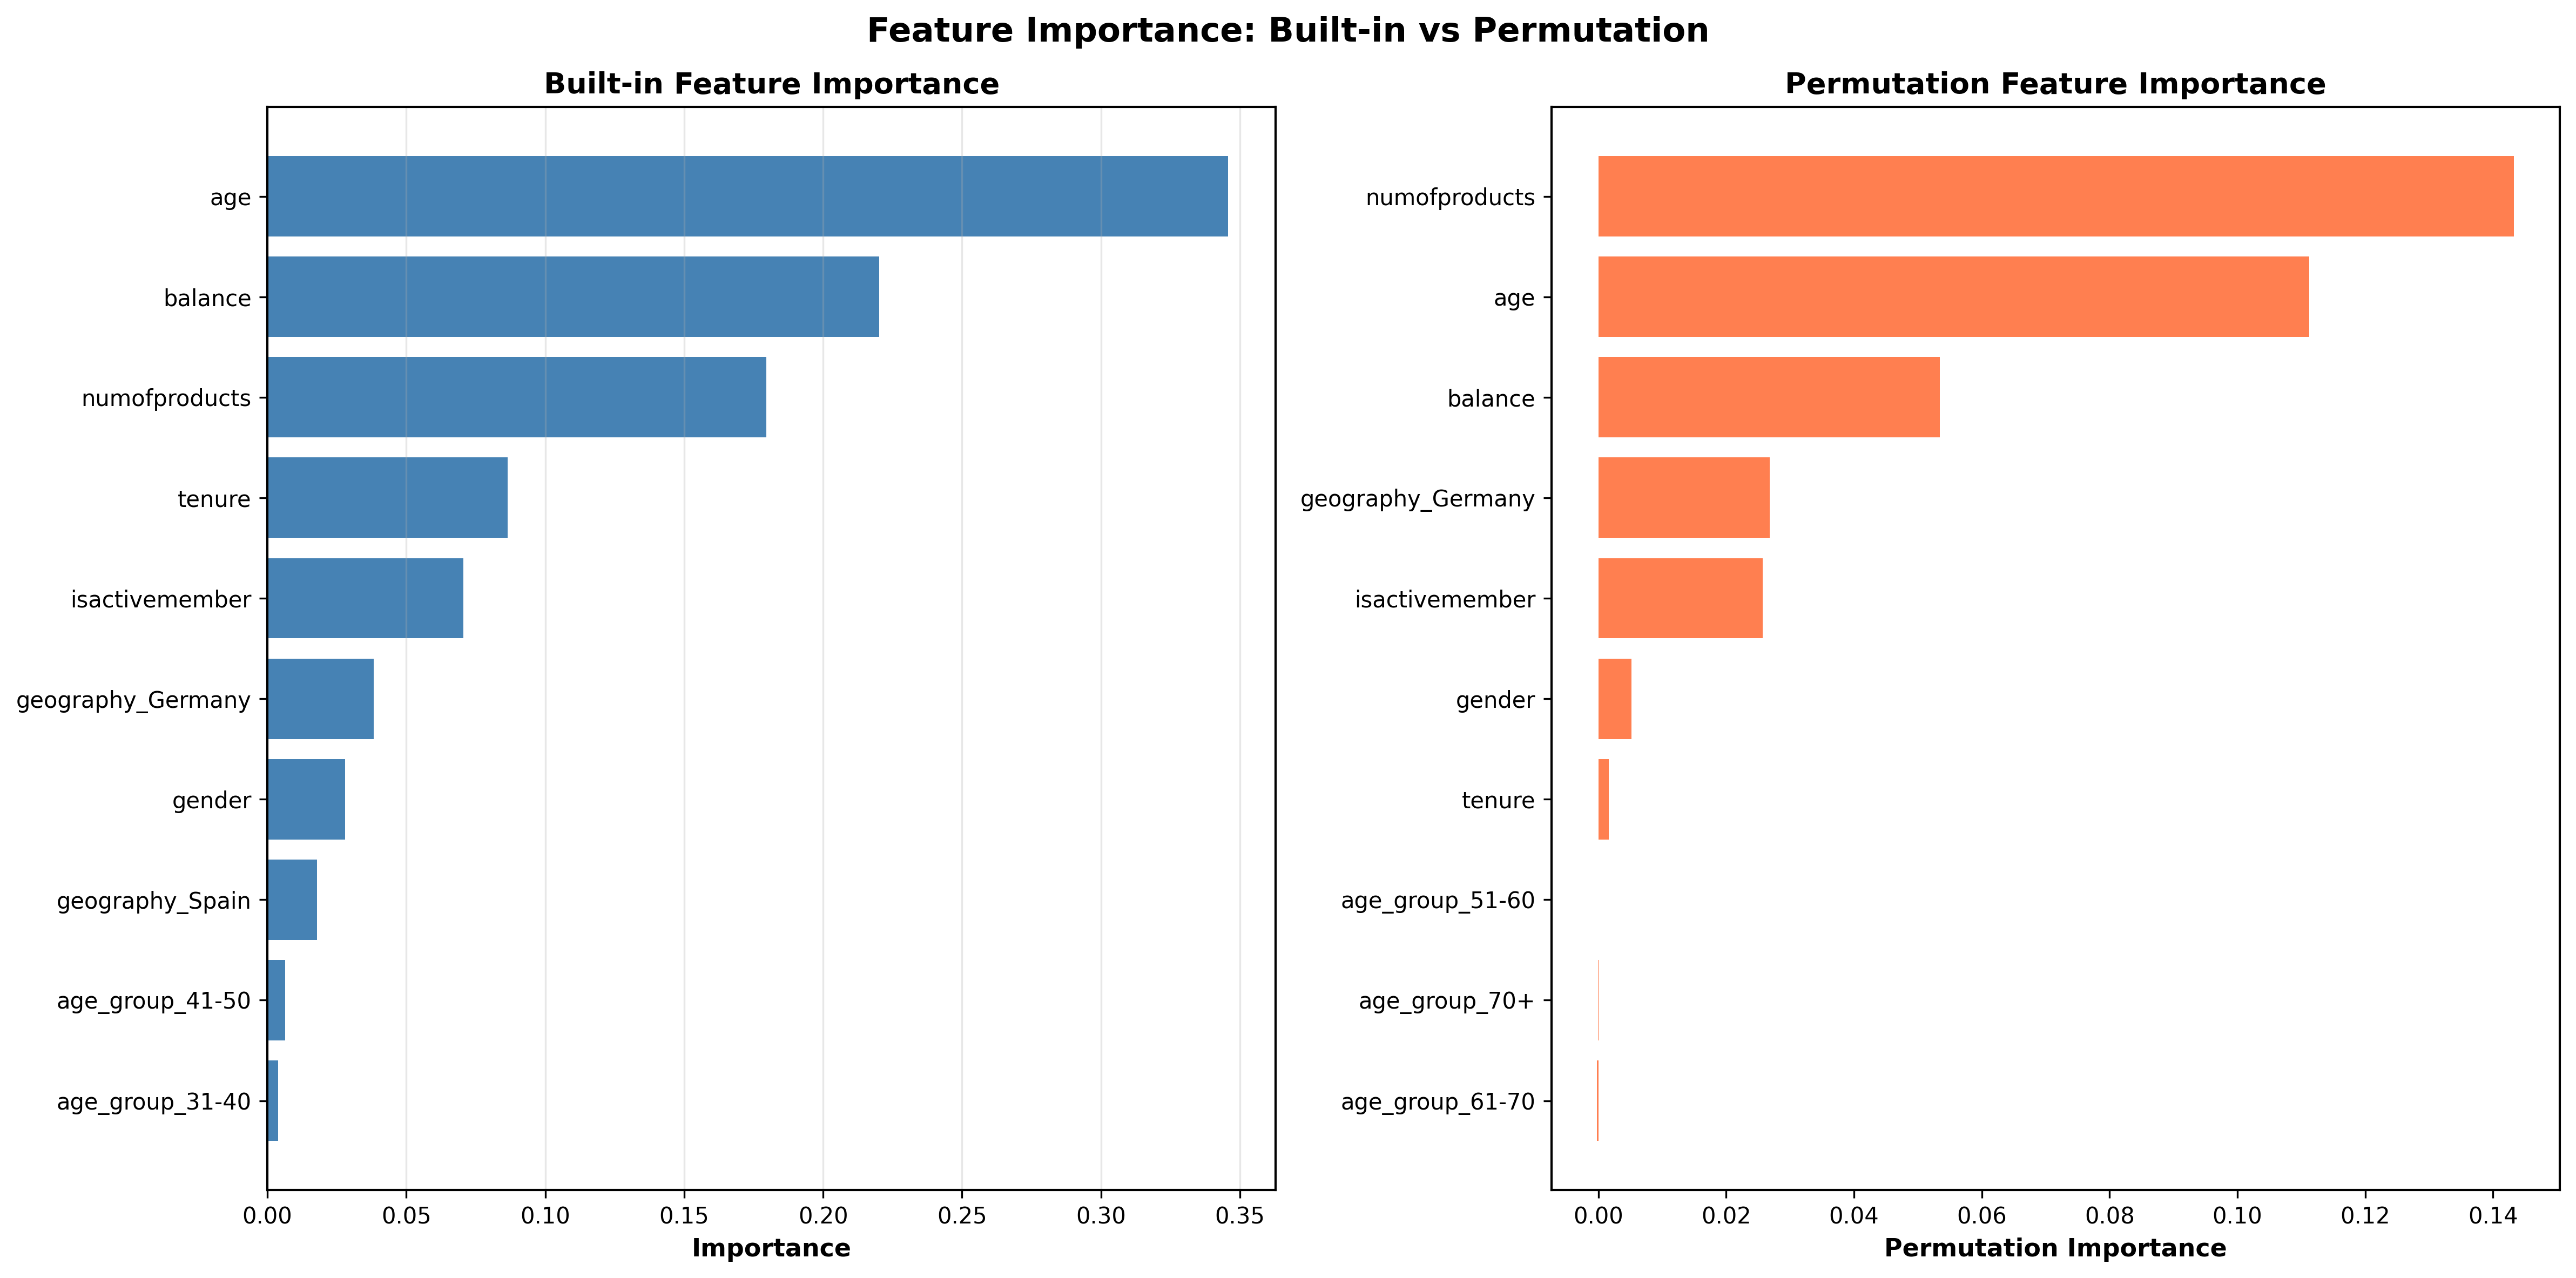
\includegraphics[width=0.8\textwidth]{../img/15_feature_importance_comparison.png}
\caption{Feature importance comparison using impurity measures, permutation importance, and SHAP values. Age and number of products emerge as most influential predictors.}
\label{fig:feature_importance}
\end{figure}

\begin{figure}[H]
\centering
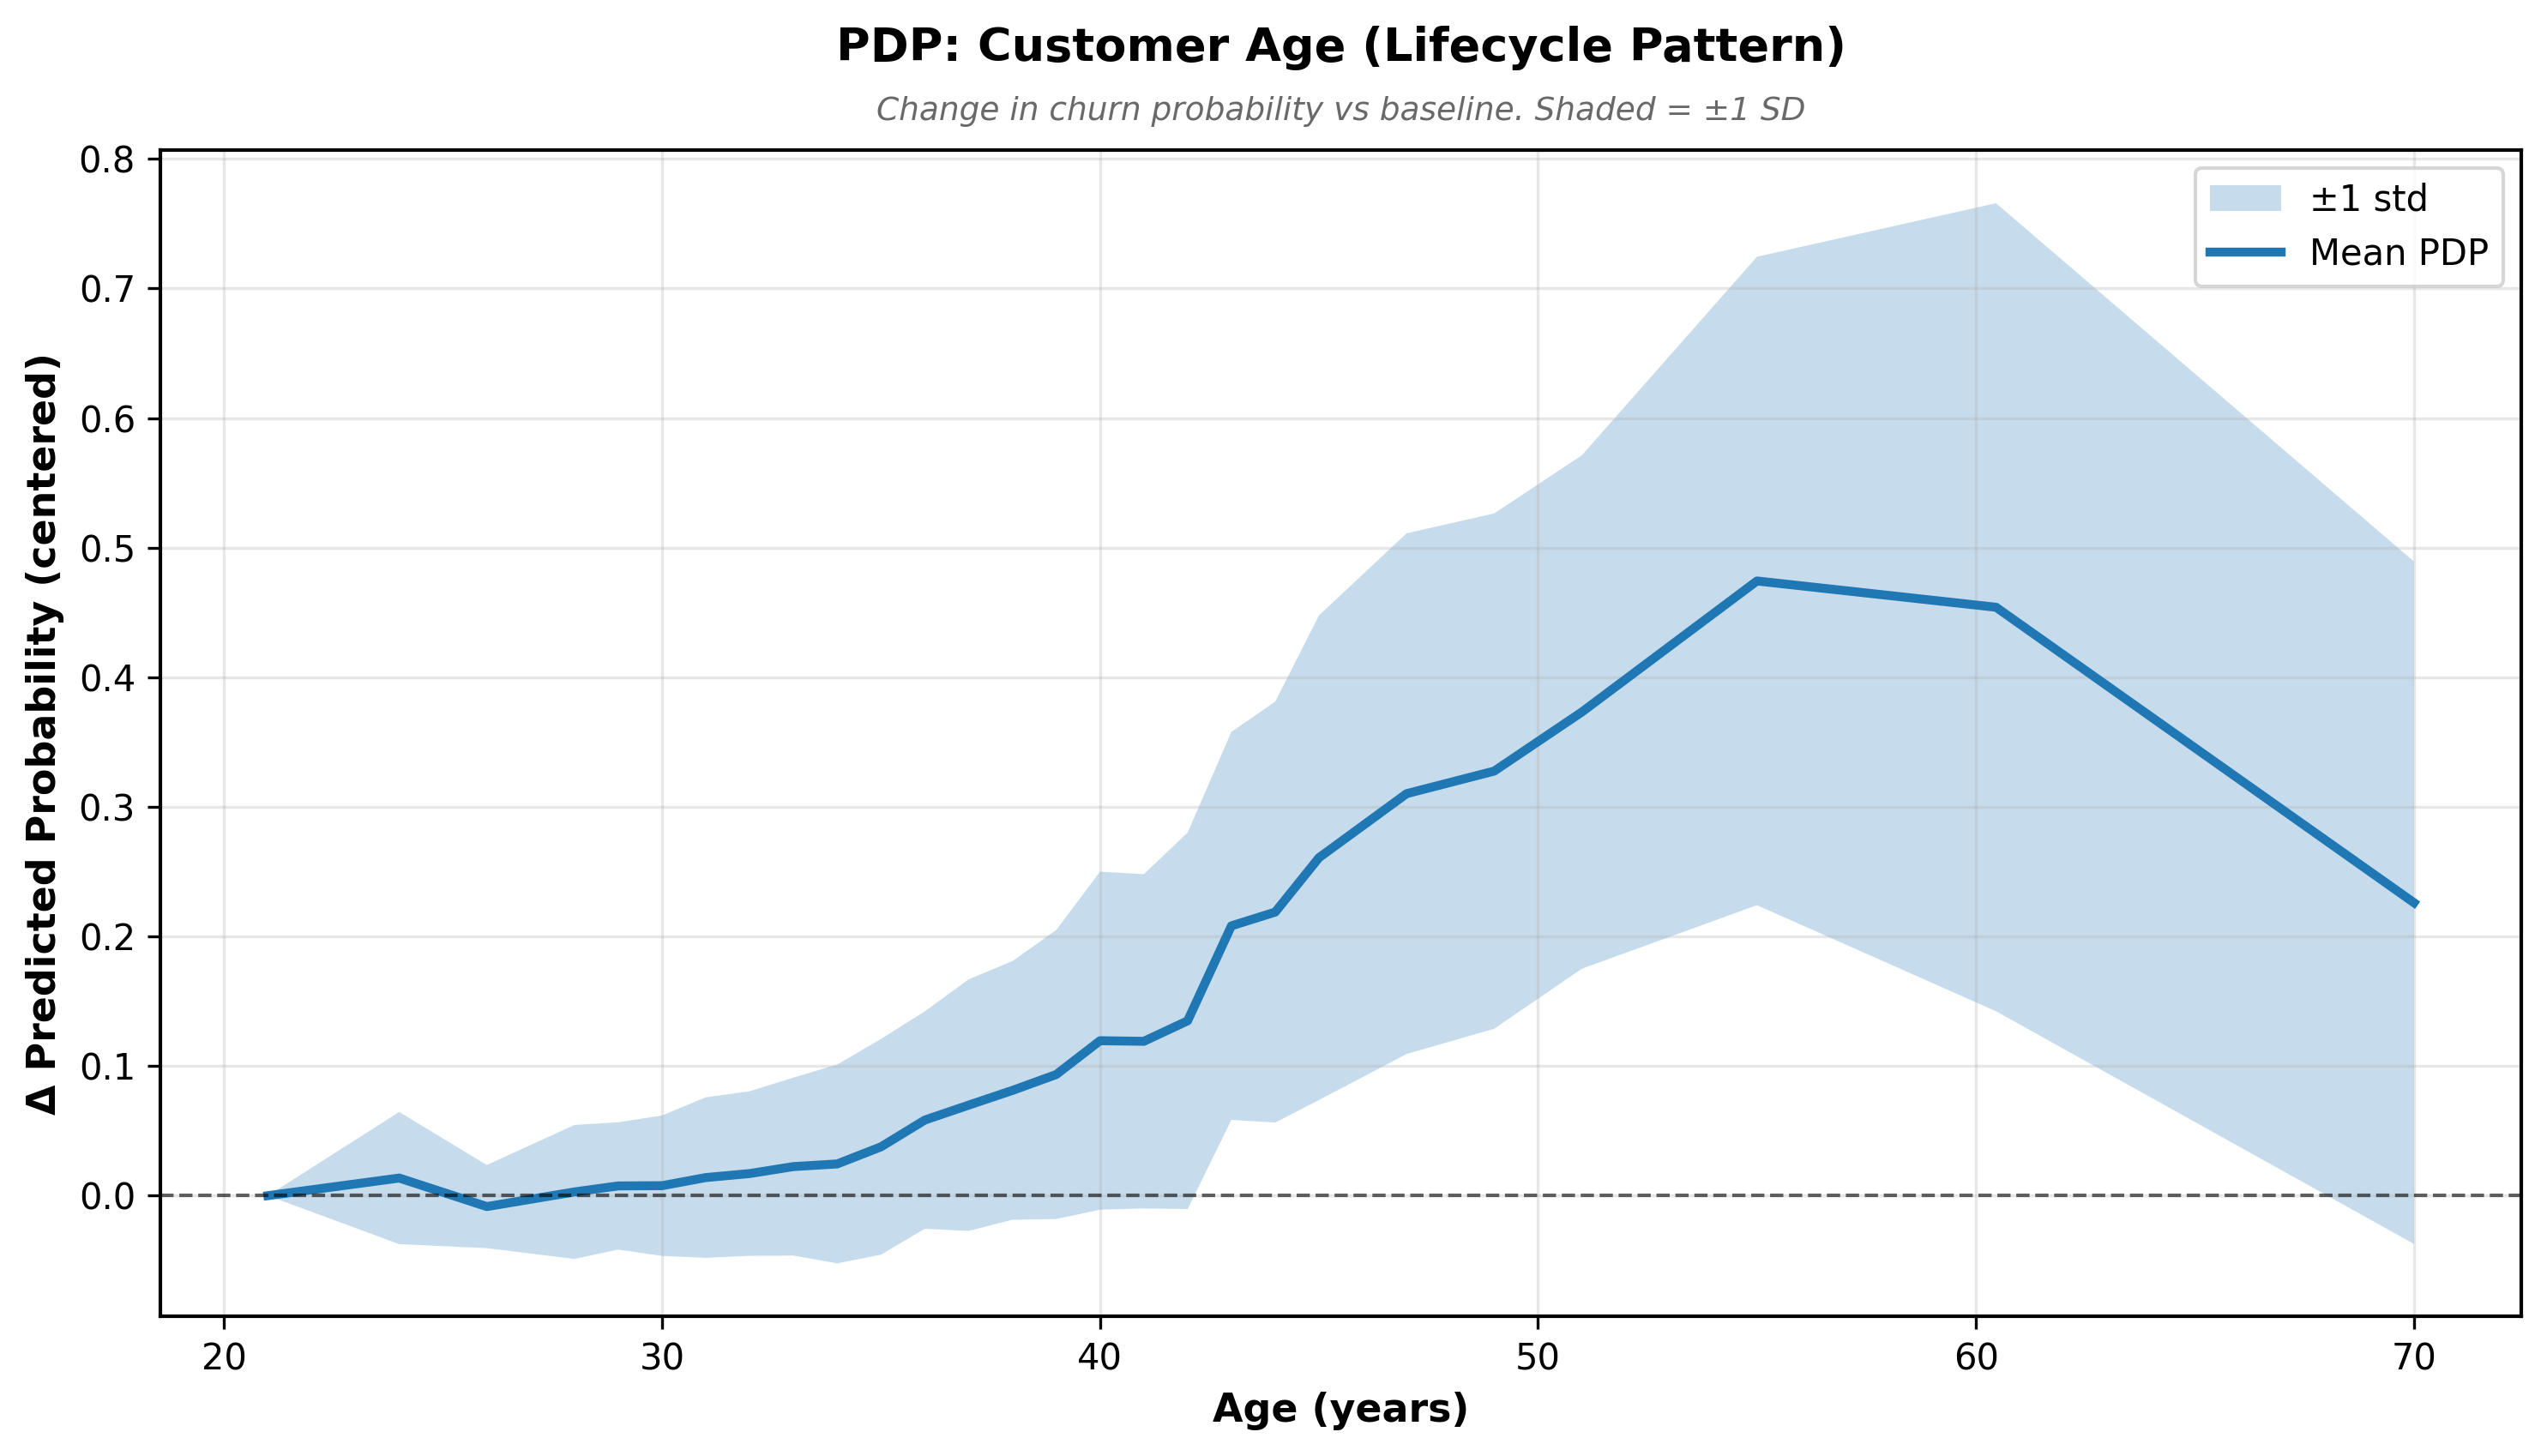
\includegraphics[width=0.6\textwidth]{../img/18_pdp_age.png}
\caption{Partial dependence plot for age. Near‑monotonic increase in churn probability peaks at 51–60 years.}
\label{fig:pdp_age}
\end{figure}


\begin{figure}[H]
\centering
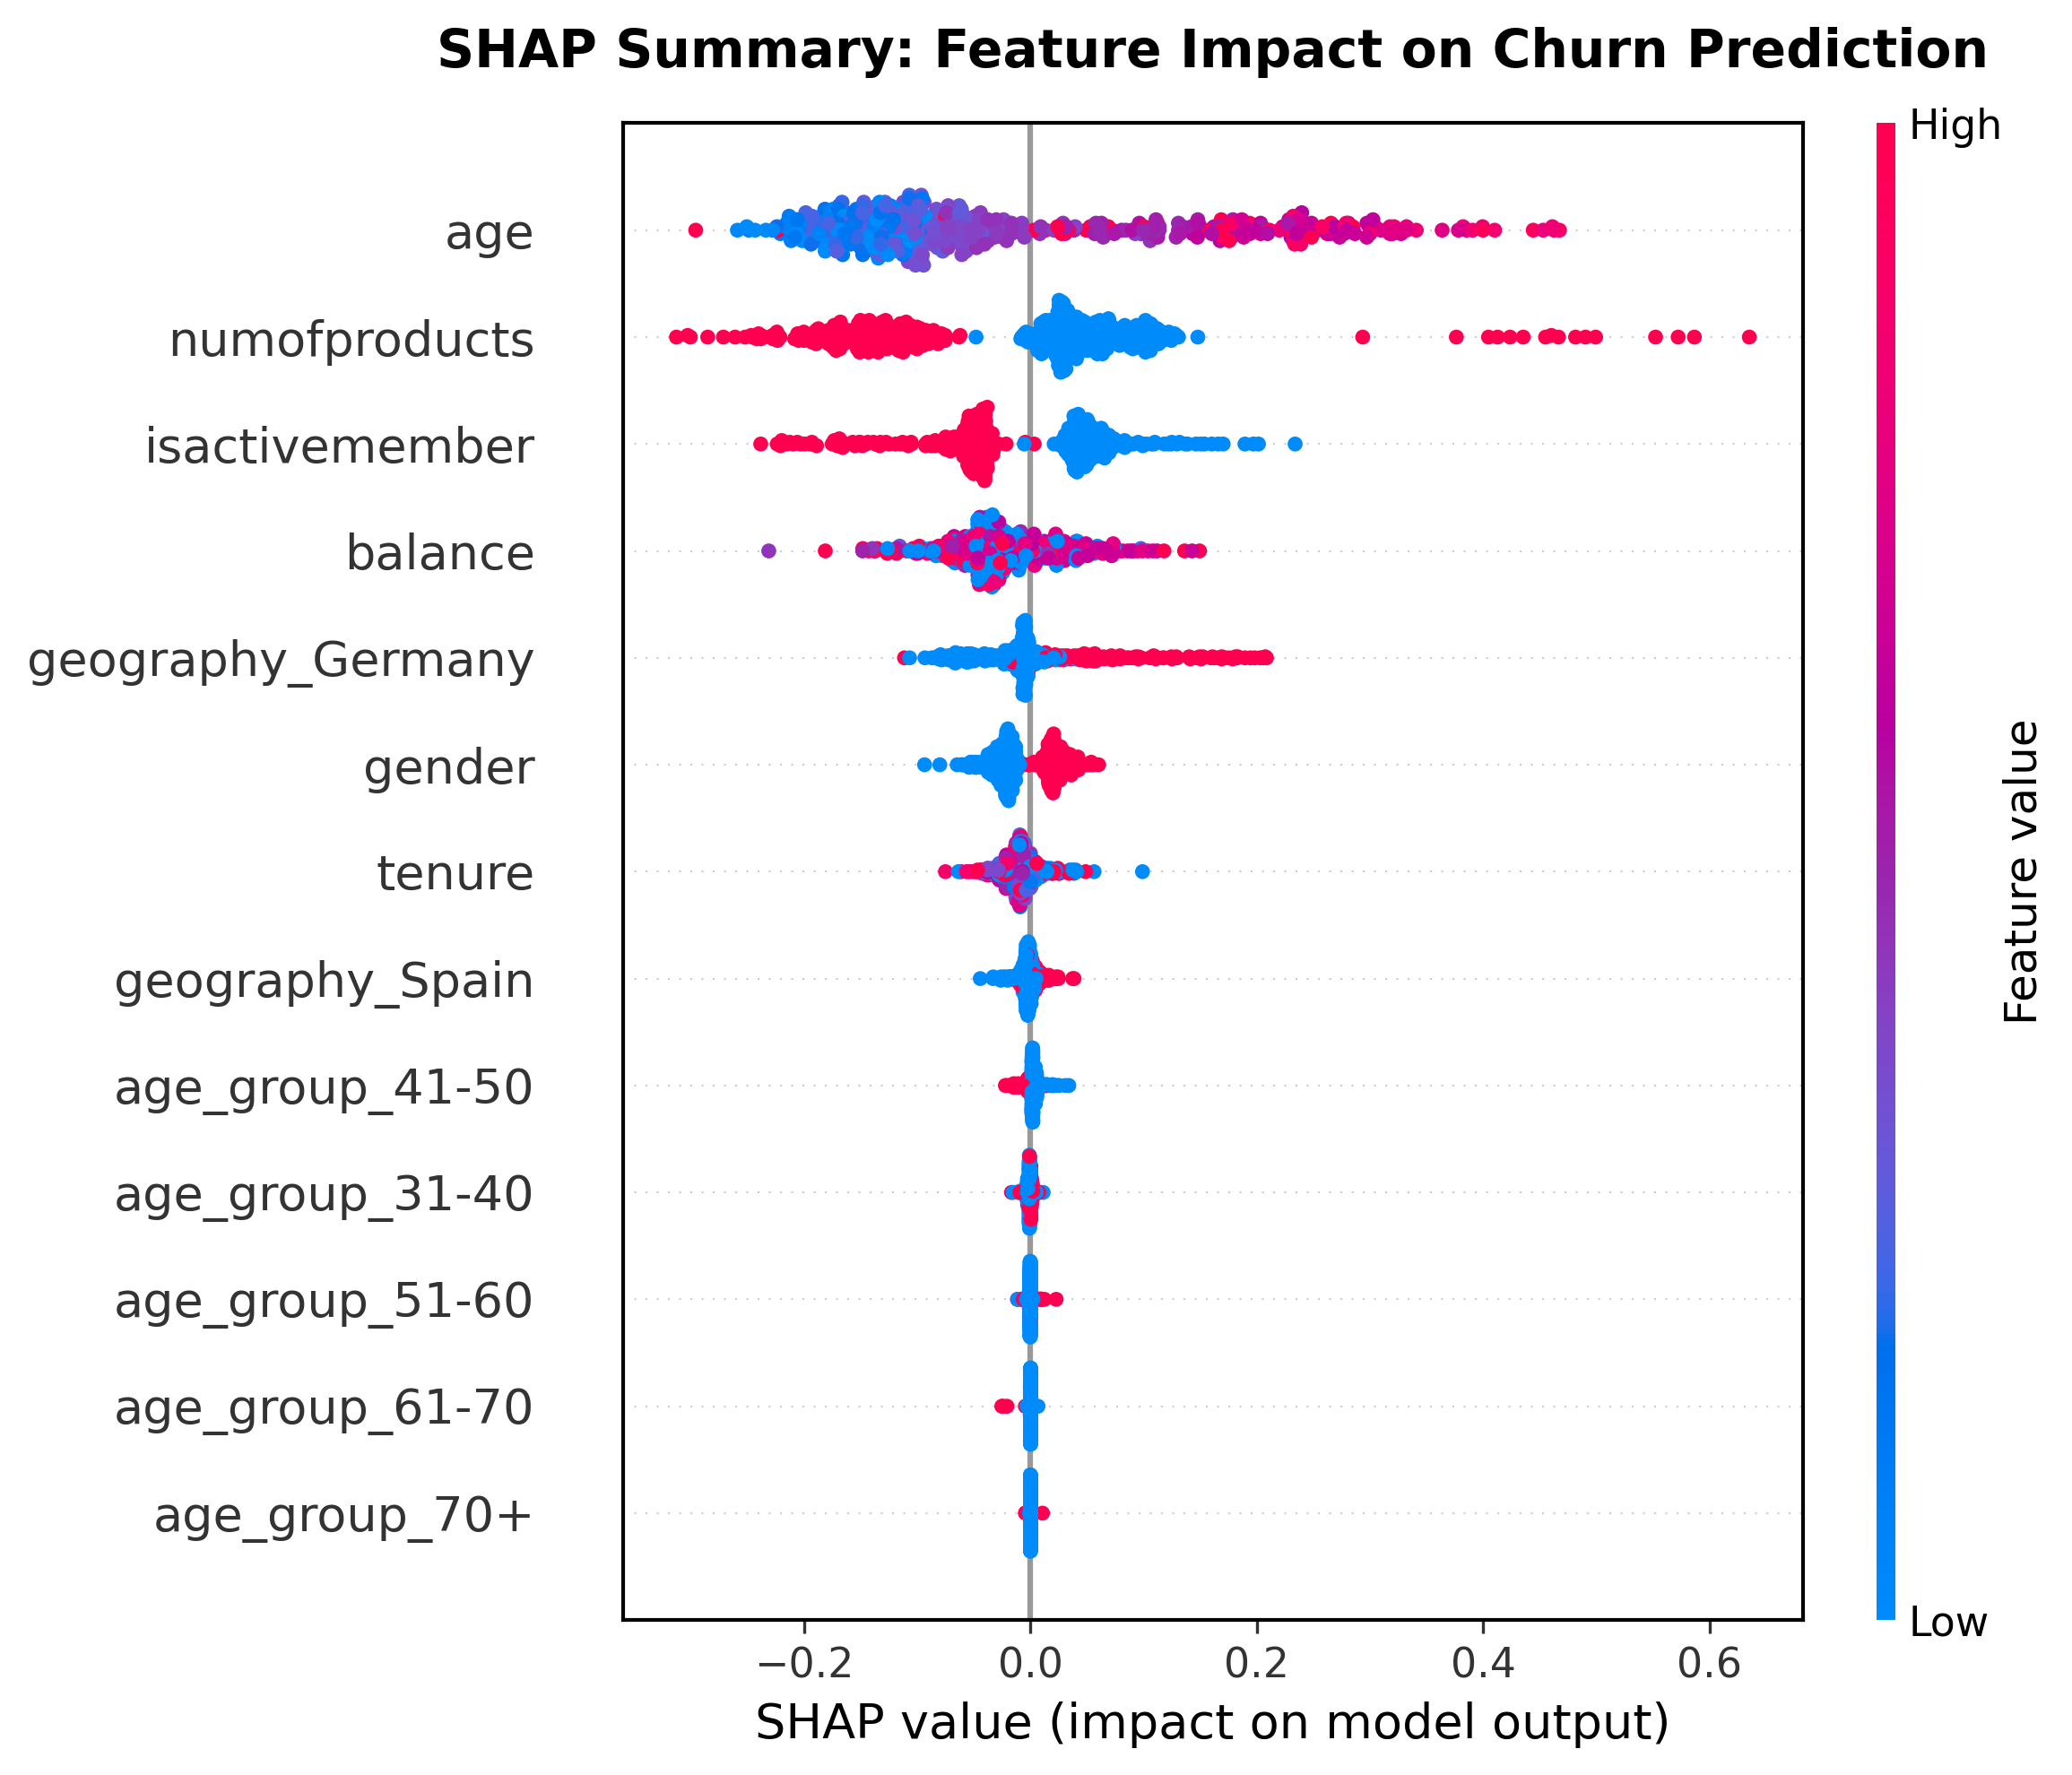
\includegraphics[width=0.7\textwidth]{../img/20_shap_summary.png}
\caption{SHAP summary plot showing feature contributions across all predictions. Blue bars indicate protective effects; red bars indicate increased churn risk.}
\label{fig:shap}
\end{figure}

The SHAP summary plot provides a population-level view of feature contributions across all customers. To illustrate how SHAP values decompose an individual prediction into feature-level contributions, Figure~\ref{fig:shap_waterfall} presents a waterfall plot for a specific customer (Customer \#0). This example demonstrates how the model's prediction is constructed step-by-step, starting from the average baseline prediction and sequentially adding or subtracting the contribution of each feature. For this customer, the low age (26 years) provides the largest protective effect (reducing churn risk by 0.145), followed by active membership status (-0.054) and high account balance (-0.037). The only risk-increasing factor is the customer's single product ownership (+0.020). These feature-level contributions sum to a final predicted probability of 7.18\%, indicating low churn risk. This customer was correctly predicted as retained, demonstrating the model's ability to identify low-risk profiles.

For operational deployment, customers can be segmented into action tiers based on predicted churn probability: low-risk ($<$20\%) receive standard service, medium-risk (20–50\%) trigger targeted re-engagement campaigns, and high-risk ($>$50\%) warrant immediate intervention with dedicated relationship managers or retention offers. This probability-based segmentation enables efficient resource allocation while ensuring high-risk customers receive priority attention.

\begin{figure}[H]
\centering
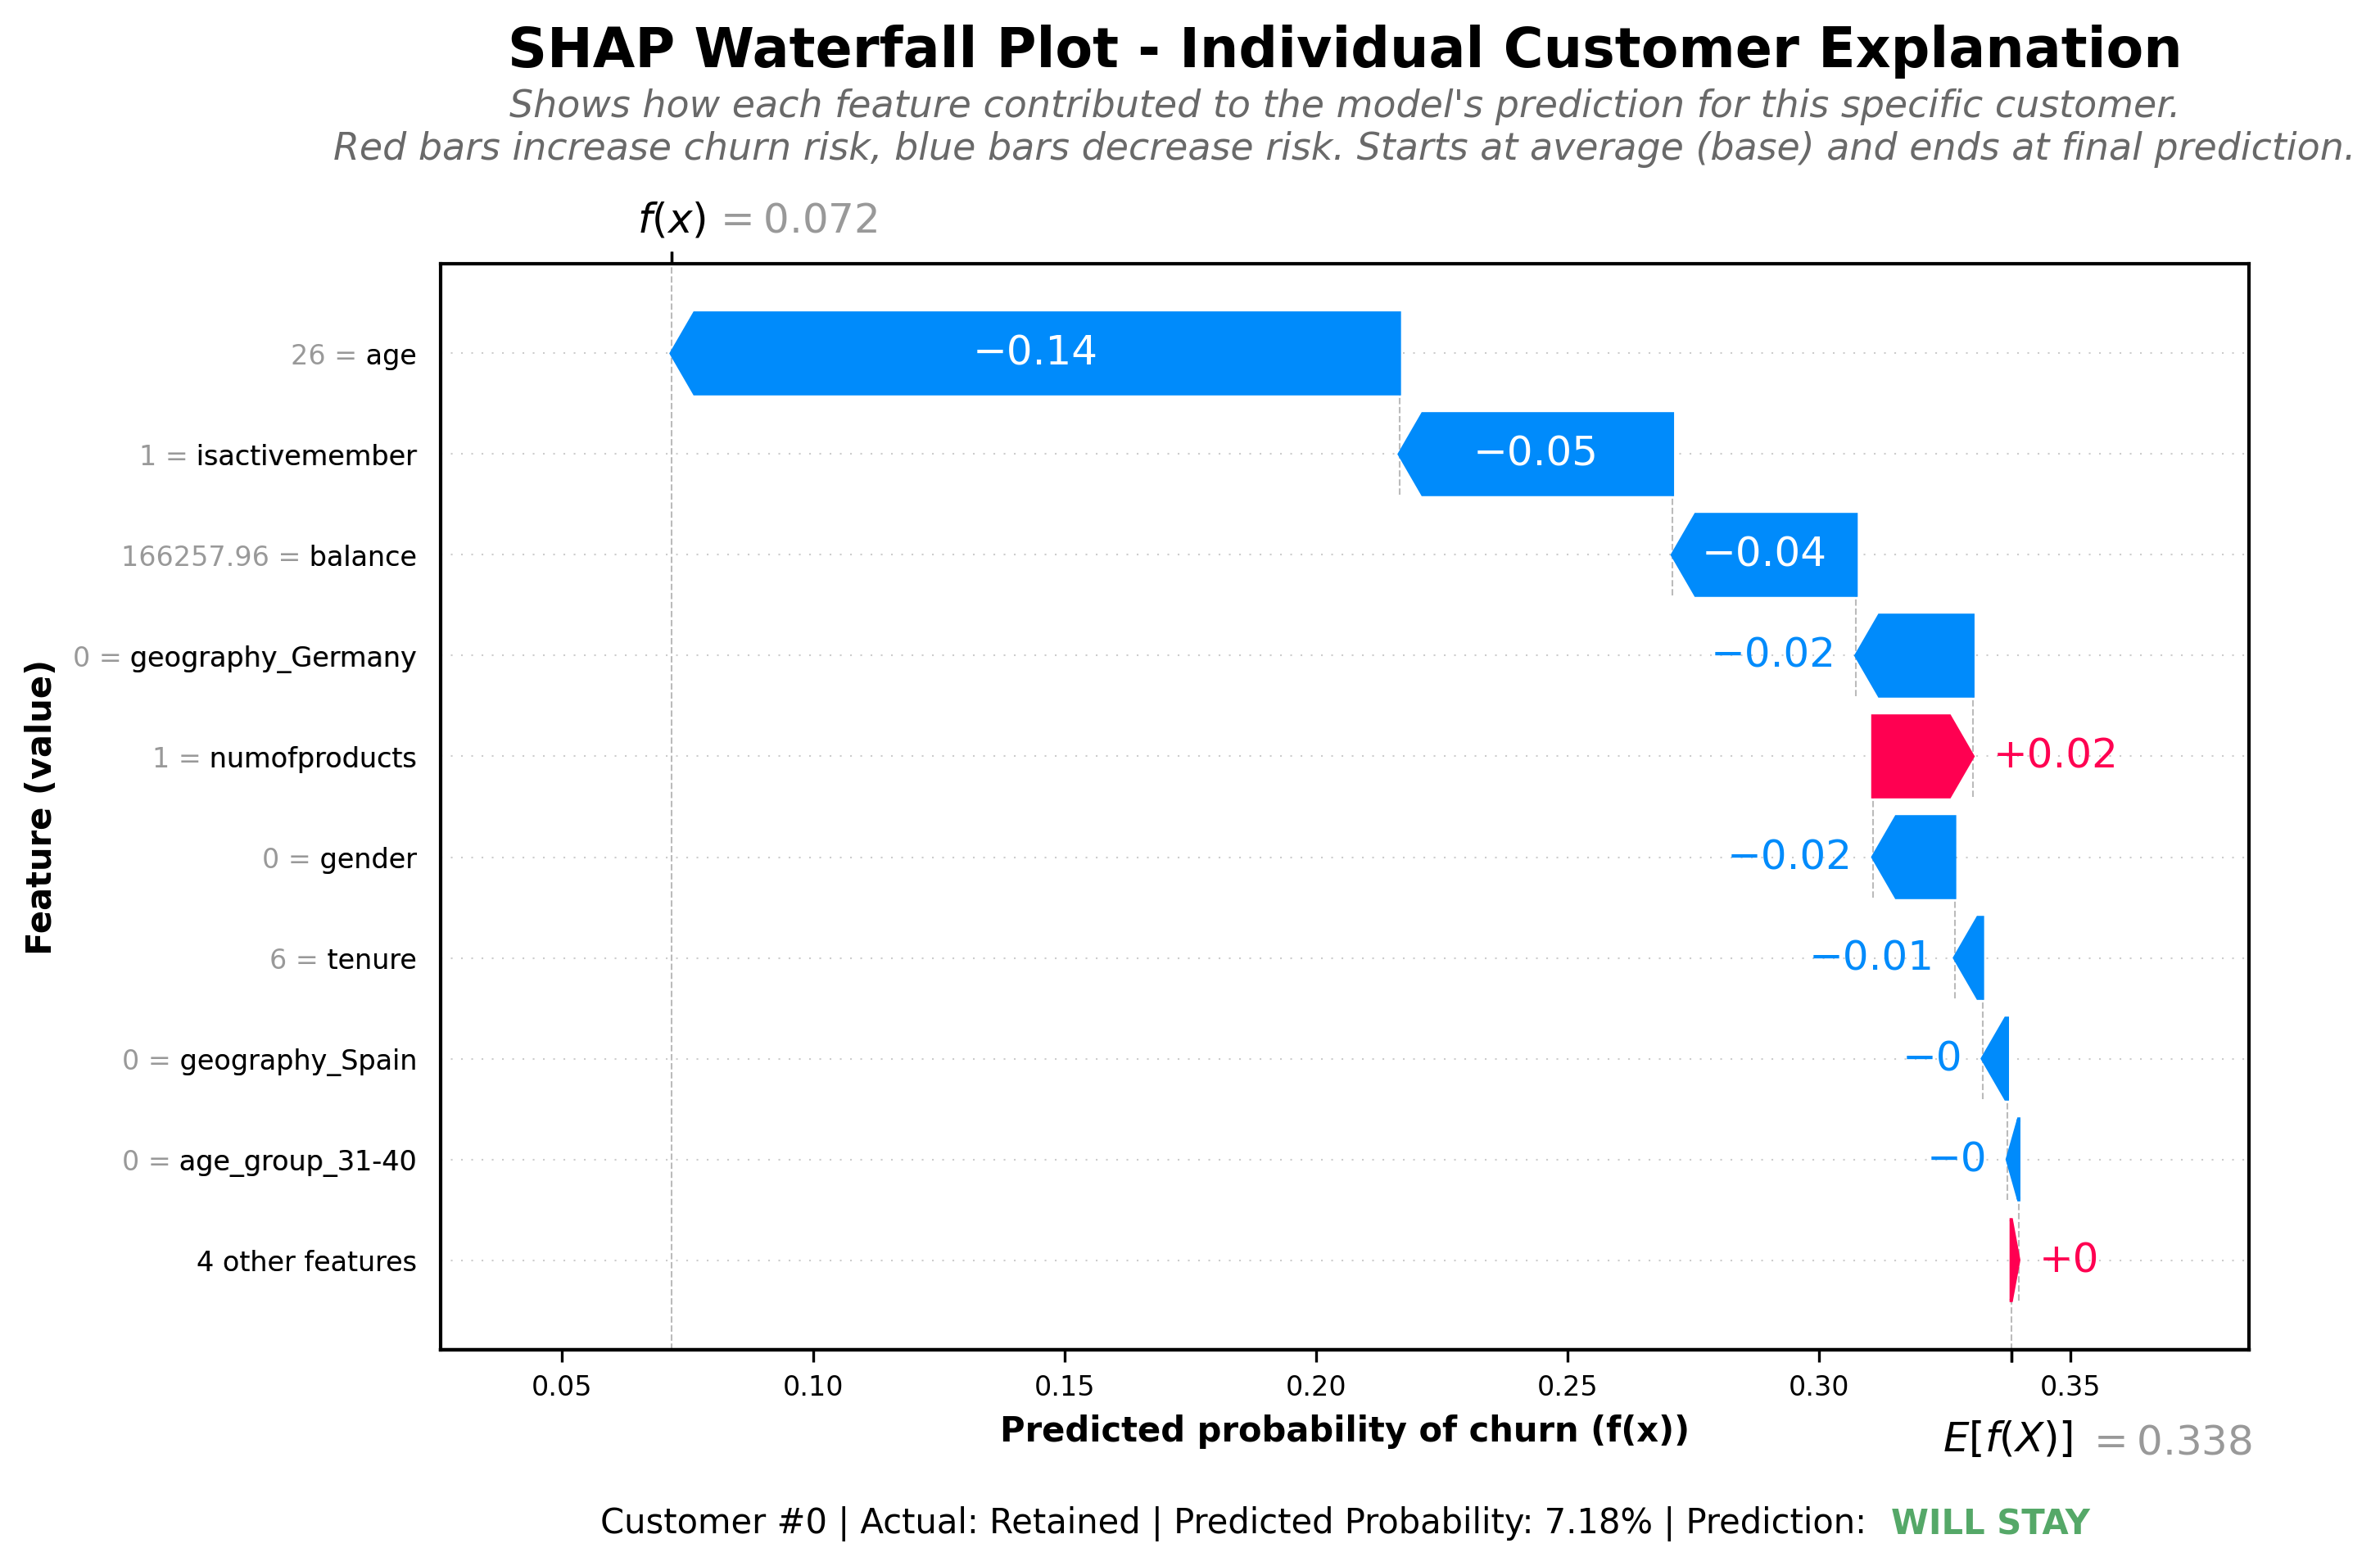
\includegraphics[width=\textwidth]{../img/26_shap_waterfall.png}
\caption{SHAP waterfall plot for individual customer prediction. Each feature's contribution appears as colored bars: blue decreases risk, red increases risk. Prediction evolves from baseline average to final probability.}
\label{fig:shap_waterfall}
\end{figure}

\begin{table}[H]
\centering
\small
\caption{Top 5 Contributing Features for Customer \#0. Features are ranked by absolute SHAP value, with positive values indicating increased churn risk and negative values indicating decreased risk. This customer was correctly predicted as retained with a 7.18\% churn probability.}
\label{tab:shap_top5}
\begin{tabular}{lccc}
\toprule
\textbf{Feature} & \textbf{Value} & \textbf{SHAP} & \textbf{Impact} \\
\midrule
Age & 26.00 & -0.145 & Decreases \\
IsActiveMember & 1.00 & -0.054 & Decreases \\
Balance & 166,257.96 & -0.037 & Decreases \\
Geography\_Germany & 0.00 & -0.023 & Decreases \\
NumOfProducts & 1.00 & +0.020 & Increases \\
\bottomrule
\end{tabular}
\end{table}

\subsection{Model Validation and Robustness Checks}
To ensure robustness, the random forest was compared against two gradient‑boosting alternatives: XGBoost and LightGBM (Figure~\ref{fig:model_comparison}).  All models were trained on identical splits and tuned with analogous hyperparameter searches.  Random forests slightly outperformed the alternatives in F1‑score (62.5~\% vs.\ 60.5–61.0~\%) and demonstrated more stable generalisation across folds.  A comprehensive metrics comparison (Figure~\ref{fig:metrics_comparison}) confirmed Random Forest's superiority.  Experiments evaluating synthetic minority oversampling (SMOTE) versus class weighting (Figure~\ref{fig:smote_roc}) revealed that SMOTE increased recall at the expense of a substantial rise in false positives; class weights offered a more balanced trade‑off.  Additional engineered features (interaction terms and polynomial expansions) did not improve performance, underscoring that tree‑based methods inherently capture non‑linear interactions.

\begin{figure}[H]
\centering
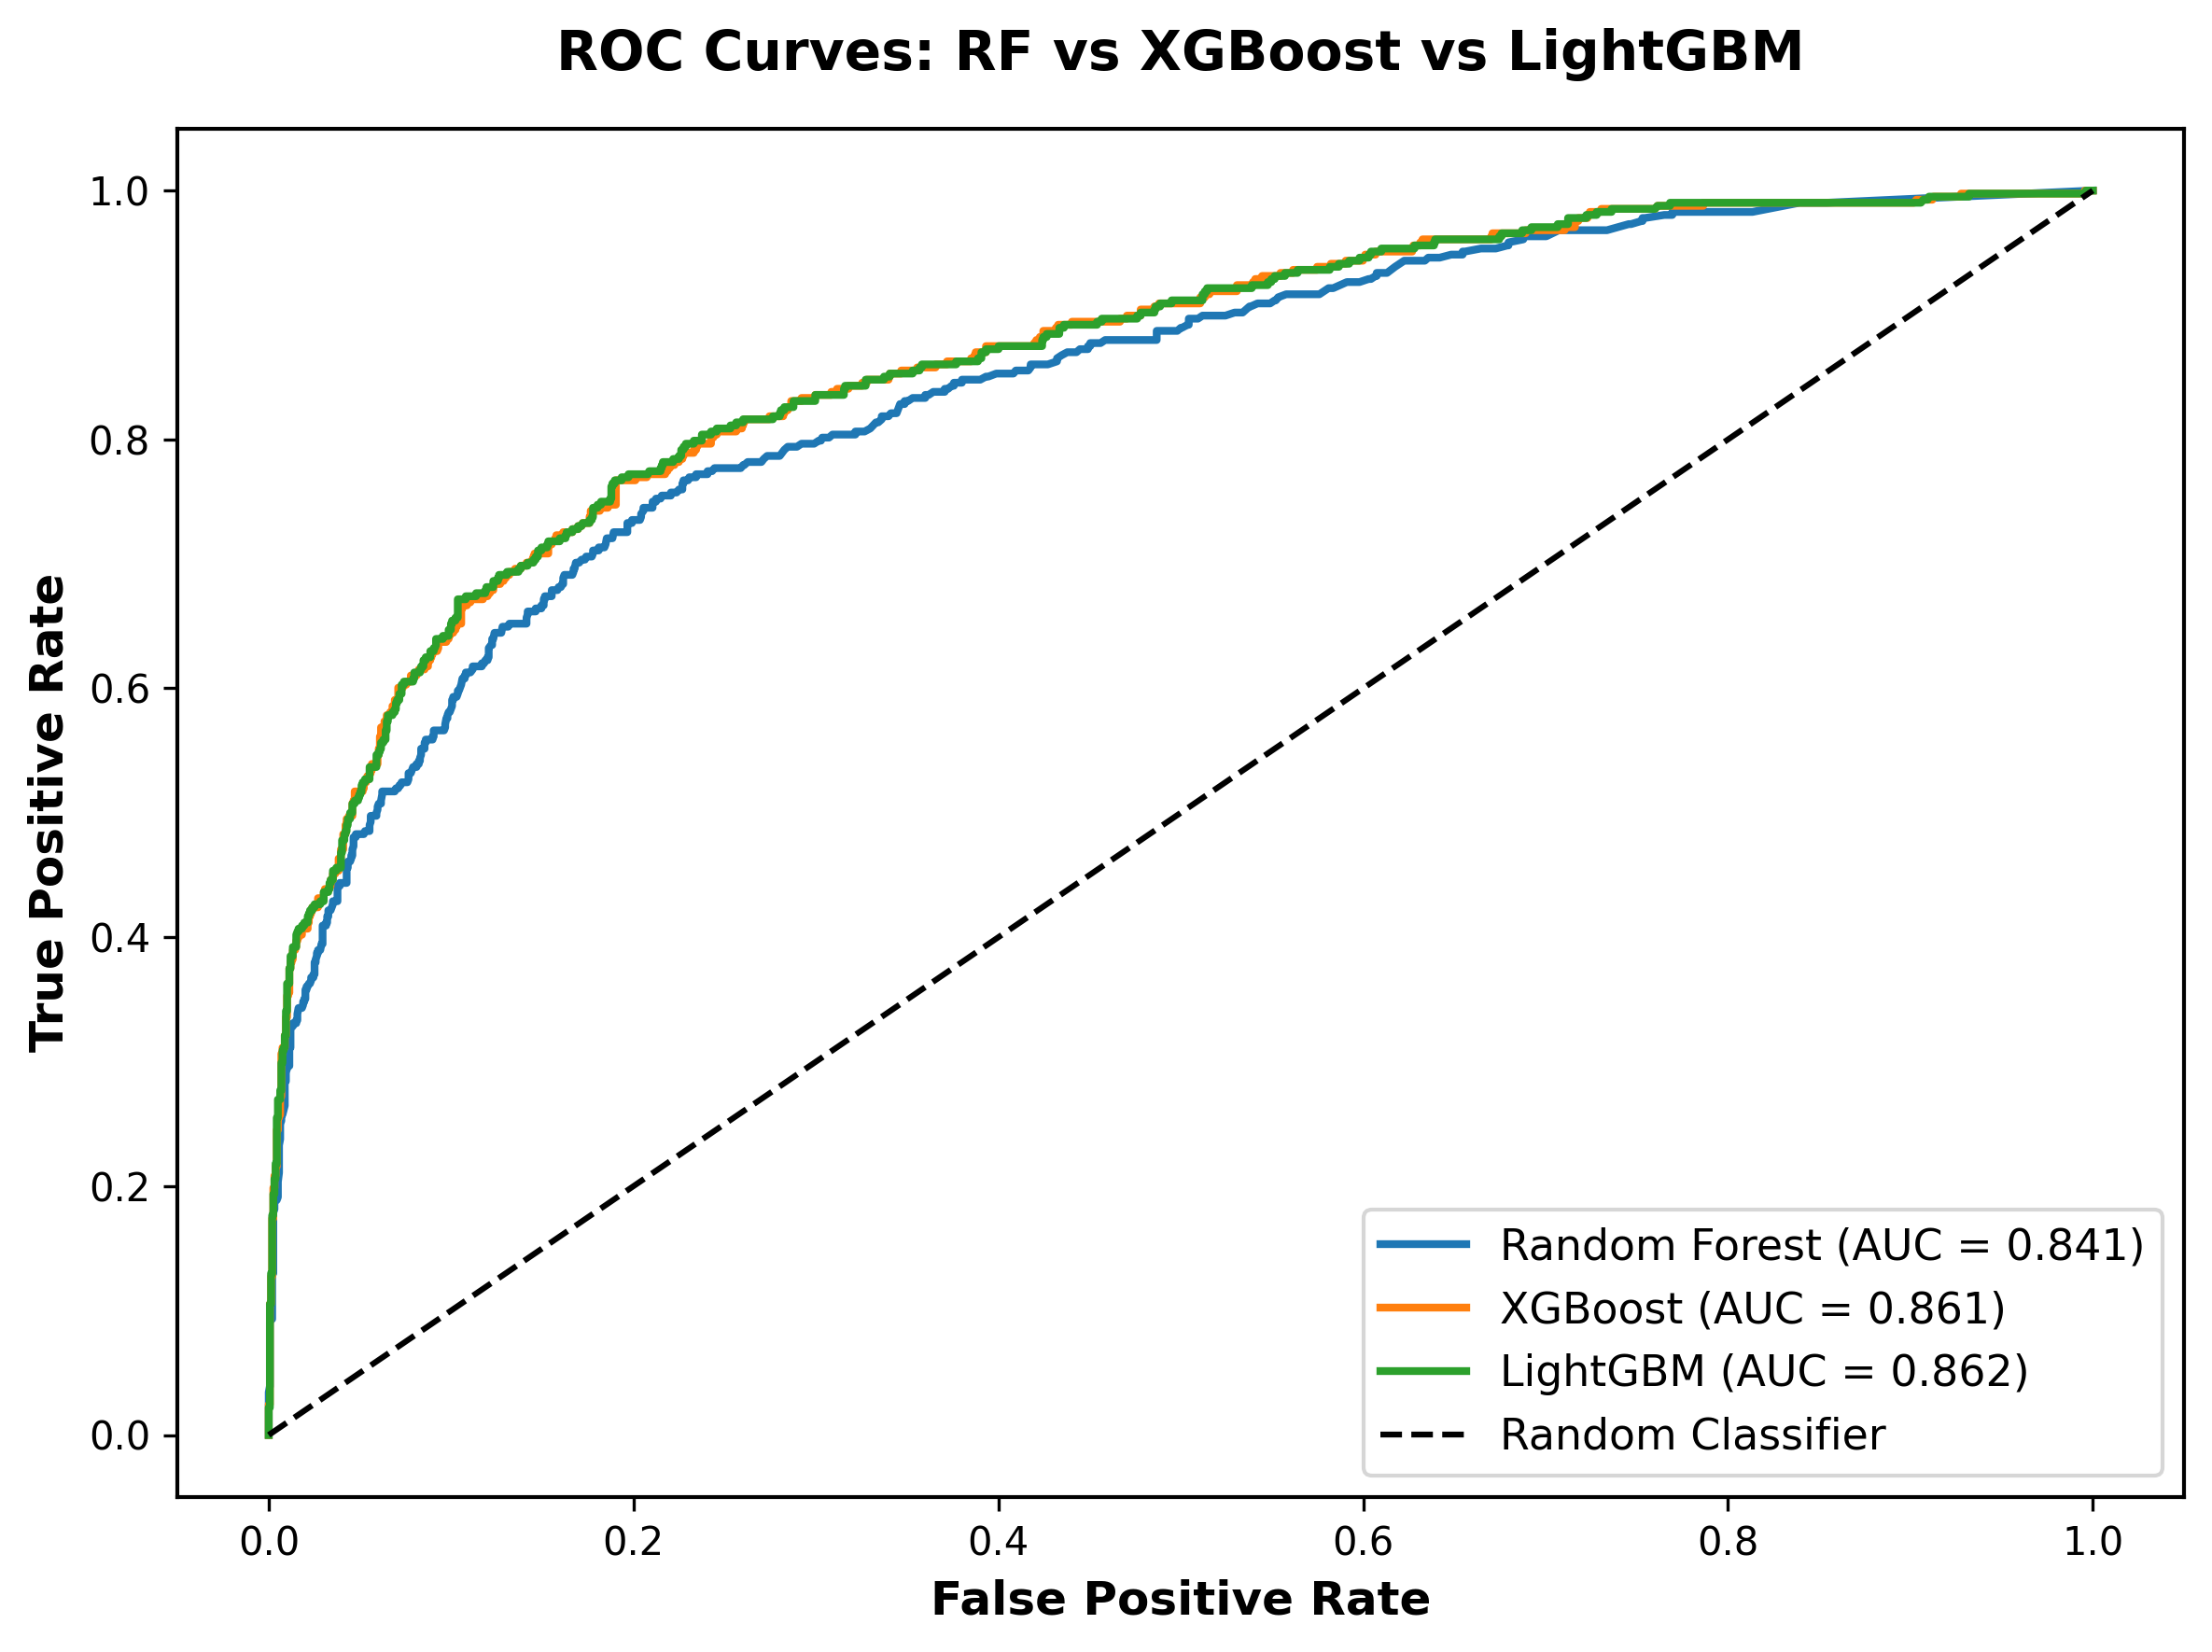
\includegraphics[width=0.7\textwidth]{../img/21_model_comparison_roc.png}
\caption{ROC curve comparison across three algorithms. Random Forest achieves highest discriminative power (AUC = 0.858).}
\label{fig:model_comparison}
\end{figure}

\begin{figure}[H]
\centering
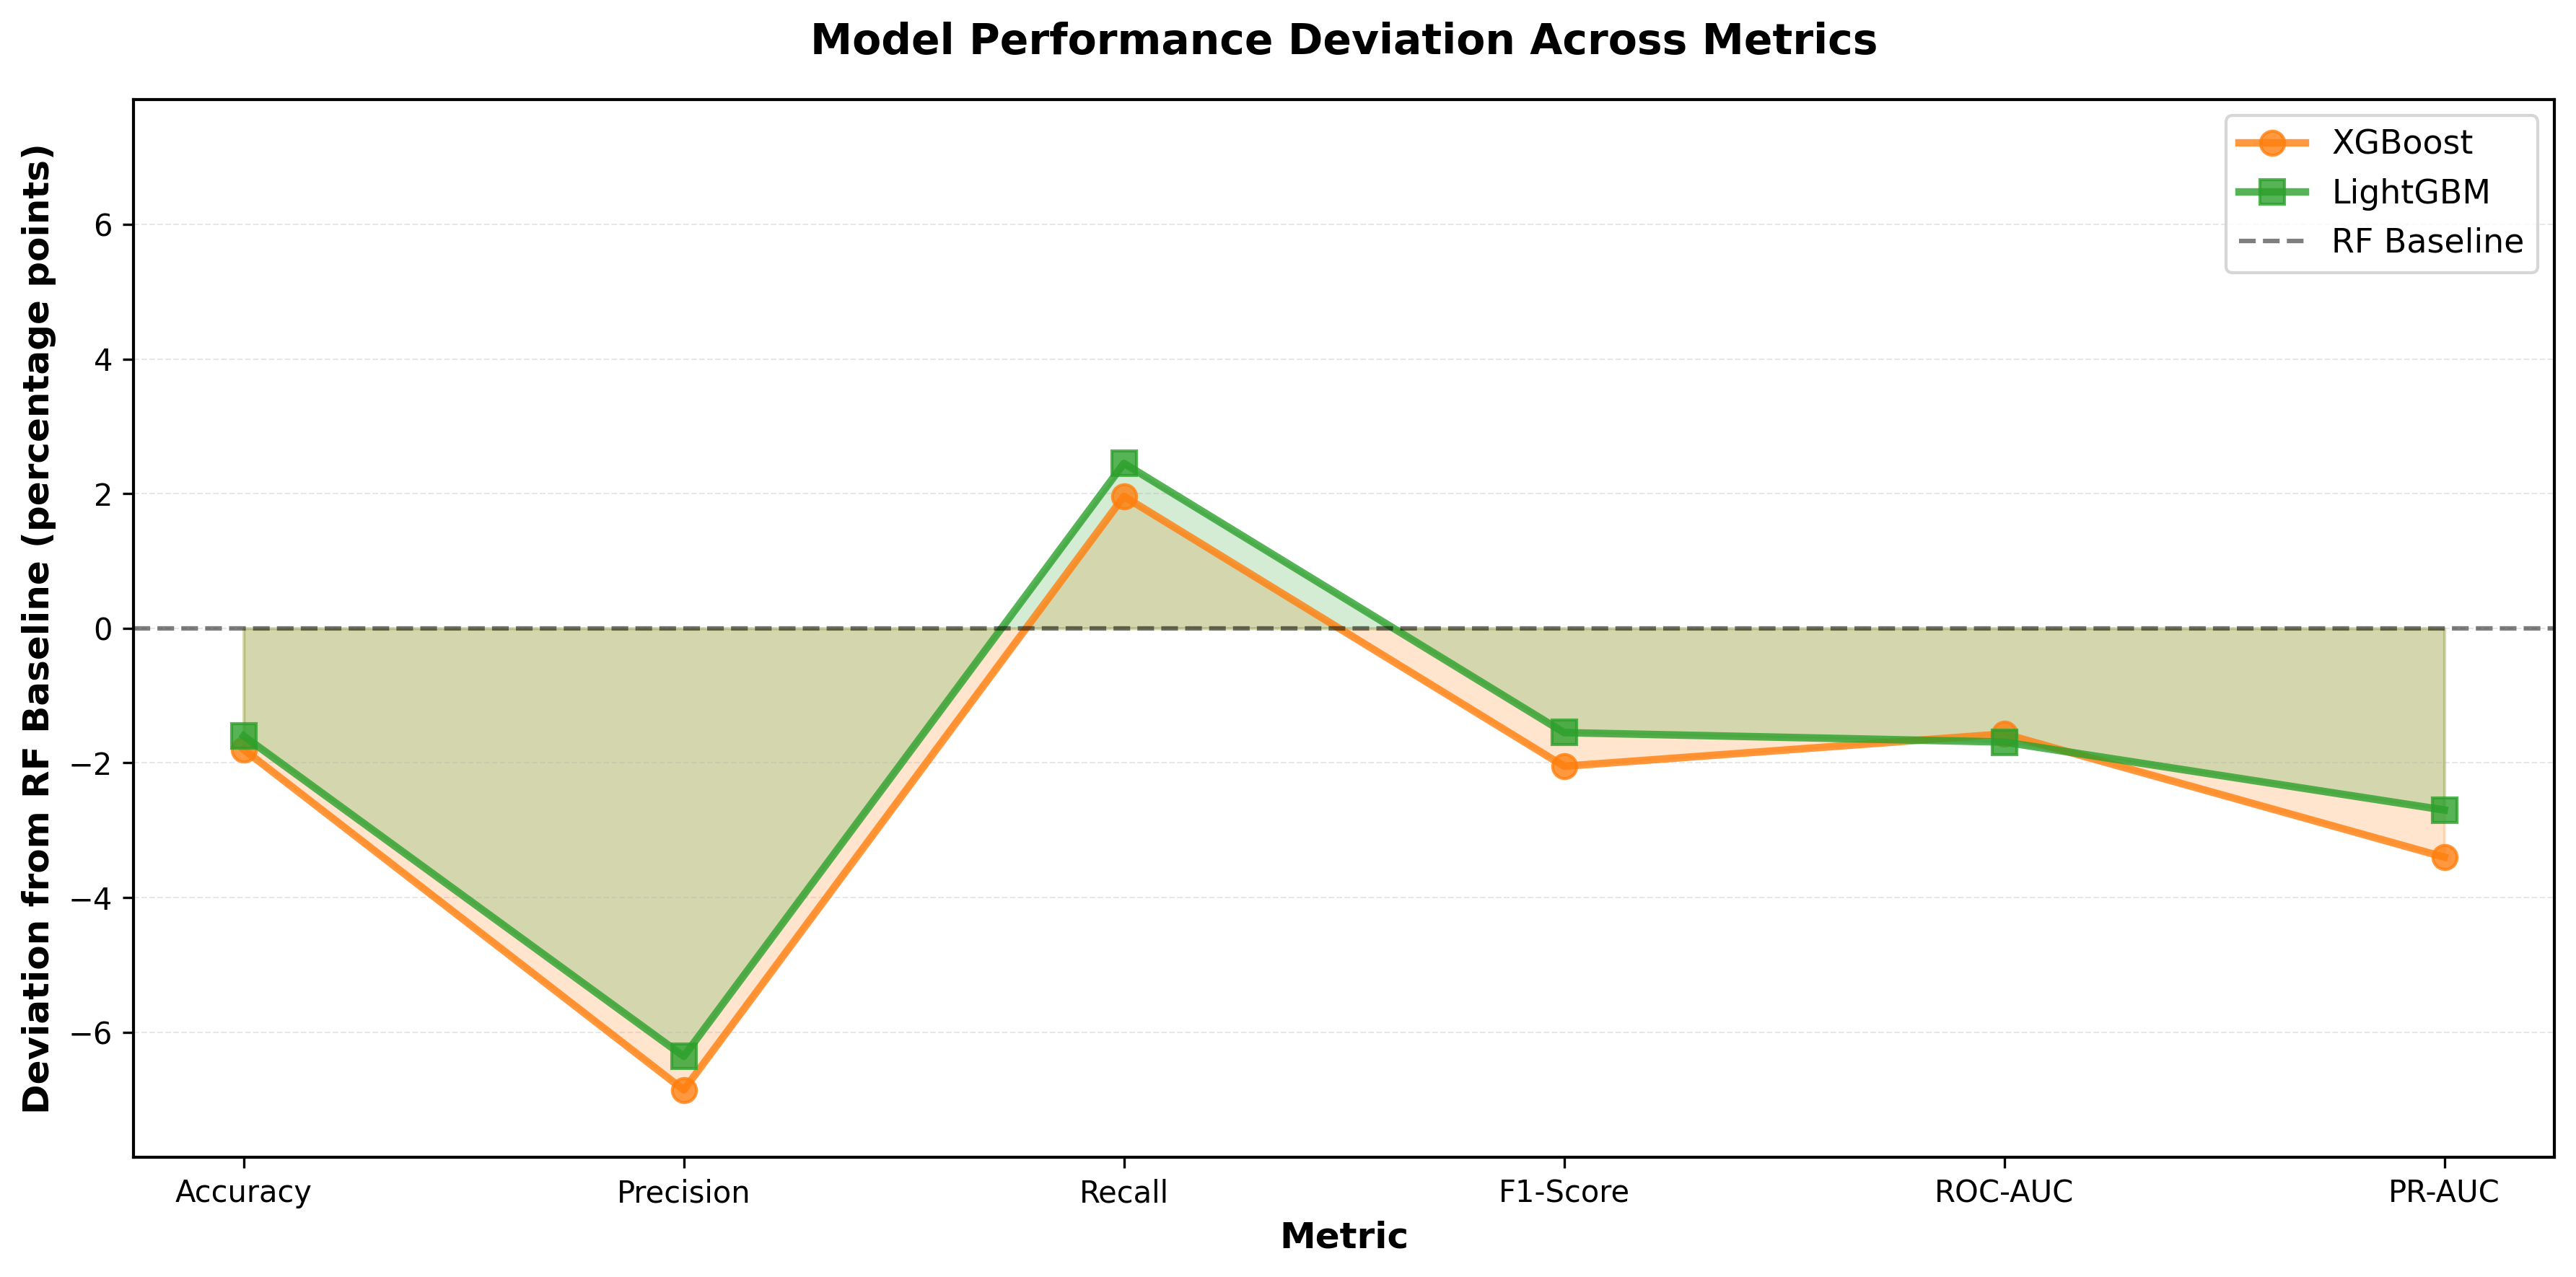
\includegraphics[width=0.9\textwidth]{../img/24_model_comparison_metrics.png}
\caption{Model performance deviation from Random Forest baseline. Both XGBoost and LightGBM underperform across most metrics.}
\label{fig:metrics_comparison}
\end{figure}

\begin{figure}[H]
\centering
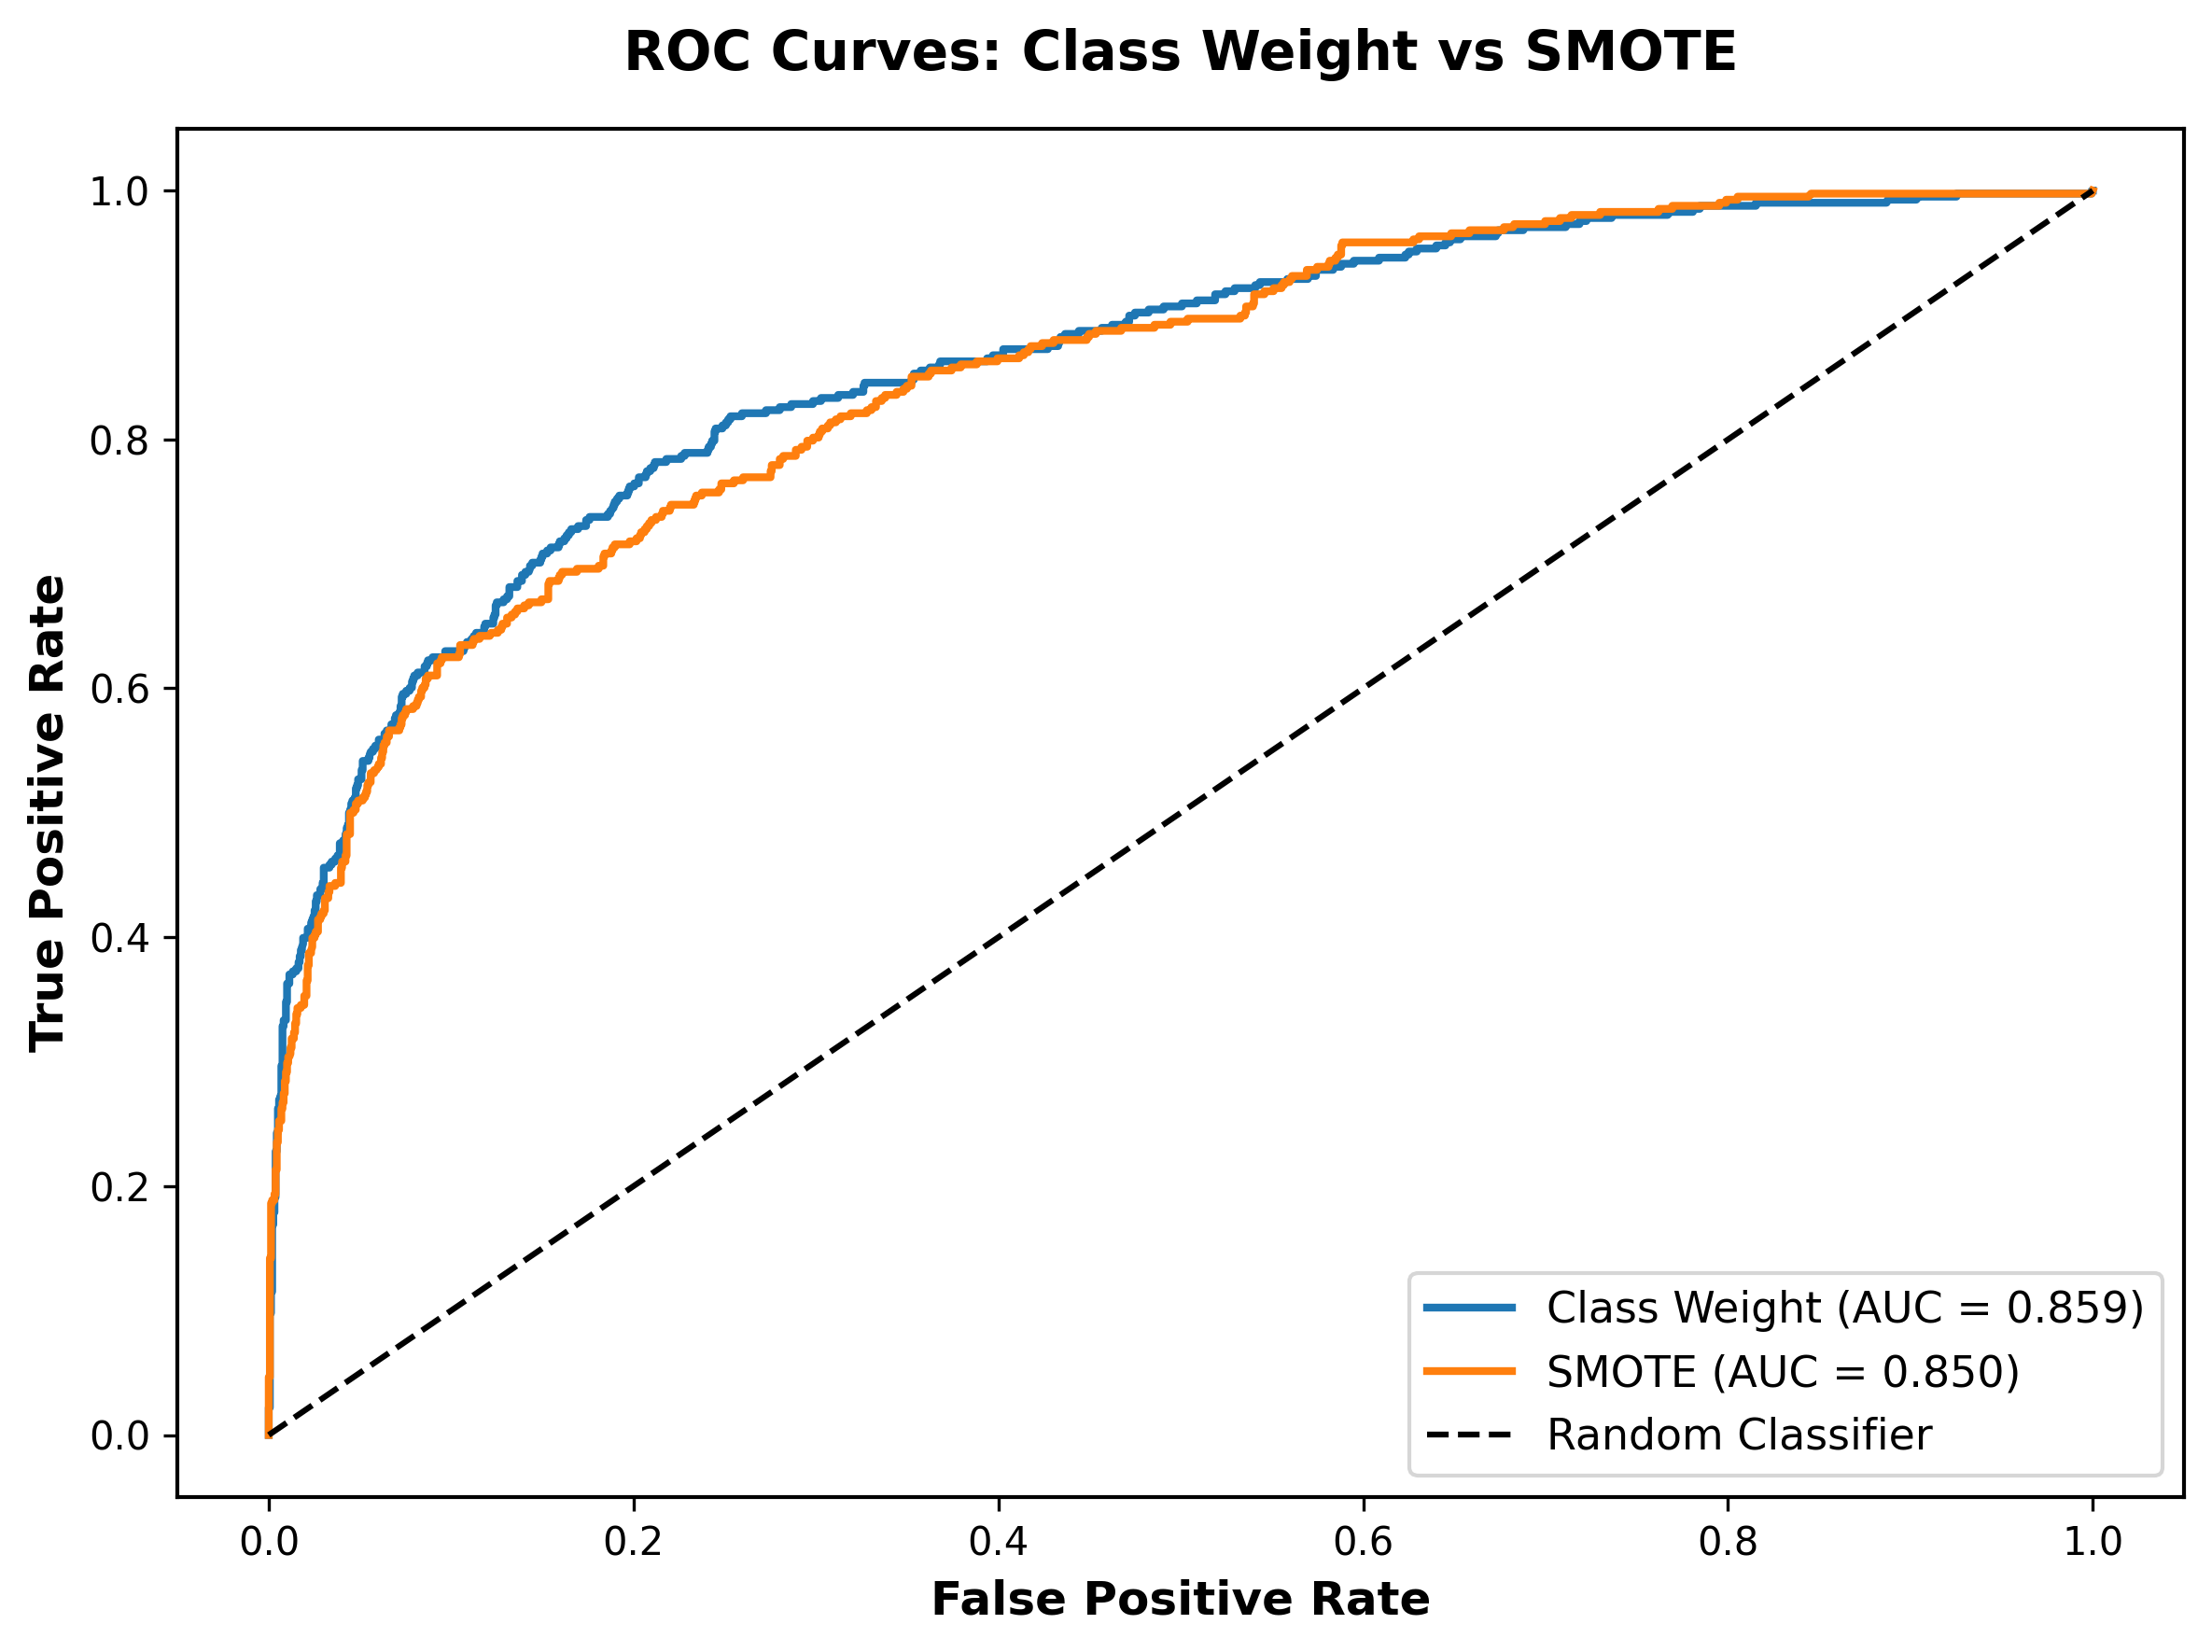
\includegraphics[width=0.7\textwidth]{../img/25_smote_roc_comparison.png}
\caption{SMOTE versus class weight ROC comparison. SMOTE increases recall at the expense of higher false positive rate.}
\label{fig:smote_roc}
\end{figure}

\section{Discussion}
\markboth{DISCUSSION}{}
\subsection{Key Findings}
The combined analyses integrating survival analysis and machine learning yielded several actionable insights:

\begin{enumerate}
  \item \textbf{Lifecycle stage drives churn risk.} The Cox model identified age as exhibiting the strongest non‑linear effect, with the 51–60 cohort showing a hazard ratio of 7.94 relative to the youngest group. This demographic corresponds to pre‑retirement customers who may consolidate assets or seek better retirement products elsewhere.

  \item \textbf{Customer engagement is the strongest modifiable predictor.} Active membership reduces churn hazard by 46\% (HR=0.54) relative to inactive members. This finding is particularly actionable because engagement can be influenced through targeted re‑activation campaigns.

  \item \textbf{Geography exhibits pronounced disparities.} German customers exhibited twice the churn rate of French and Spanish customers and a hazard ratio of 1.60. Market‑specific issues such as competition, regulation or service quality likely underlie this disparity.

  \item \textbf{Product portfolio exhibits a Goldilocks effect.} Kaplan–Meier curves revealed that customers with exactly two products displayed the lowest churn rate (7.6\%, n=4,590), whereas those with three or four products showed substantially higher attrition (82.7\% and 100\% respectively, with small sample sizes n=266 and n=60). The Cox model's linear treatment of number of products (HR=1.02) masked this underlying U‑shaped pattern, highlighting the value of non‑parametric survival analysis for uncovering non‑linear relationships.

  \item \textbf{Feature selection prioritizes actionable intelligence over accuracy.} Complaint status exhibited near‑perfect correlation with churn (r=0.996) but was intentionally excluded from predictive models as a lagging indicator. This methodological decision, which sacrifices potential 99\%+ accuracy for 85.9\%, enables identification of antecedent patterns that drive intervention strategies before customers reach the point of no return.
\end{enumerate}

These findings are supported by both the survival model and the random forest classifier, reinforcing the validity of the patterns across methodological approaches. Importantly, the risk factors vary in modifiability: age and geography are inherent, whereas number of products and activity status are under managerial control. Effective retention strategies should therefore prioritize modifiable drivers.

\subsection{Business Applications and Strategic Implications}
The statistical findings translate into actionable business intelligence through customer segmentation, targeted interventions, and quantified ROI projections. This section bridges the analytical insights with strategic recommendations for bank management.

\subsubsection{Customer Risk Profiles}
Using the predicted probabilities from the random forest and SHAP explanations, customers can be segmented into risk tiers (Table~\ref{tab:risk_profiles}). \textbf{Low‑risk} customers are typically 18–40 years old, active, own one or two products and reside in France or Spain; they have churn probabilities below 20\%. \textbf{Medium‑risk} customers are 40–55, inactive or semi‑active, own only one product and have short tenure; their churn probabilities range from 30–60\%. \textbf{High‑risk} customers are 55–70, inactive, either under‑serviced (one product) or potentially over‑serviced (three to four products) and often based in Germany; their churn probabilities exceed 70\%. Note that customers with three to four products constitute a small subgroup (n=326) and warrant targeted investigation rather than broad assumptions.

\begin{table}[H]
\centering
\small
\caption{Customer risk segmentation and intervention strategies. Risk tiers based on Random Forest predicted probabilities and SHAP attribution. Separate escalation protocol exists for customers who have lodged complaints.}
\label{tab:risk_profiles}
\begin{tabular}{p{3.5cm}p{3.5cm}p{3.5cm}p{3.5cm}}
\toprule
\textbf{Attribute} & \textbf{Low Risk} & \textbf{Medium Risk} & \textbf{High Risk} \\
\midrule
\rowcolor{gray!8}\textbf{Churn Prob.} & $<$20\% & 30-60\% & $>$70\% \\
\textbf{Age} & 18-40 & 40-55 & 55-70 \\
\rowcolor{gray!8}\textbf{Activity Status} & Active & Inactive/semi-active & Inactive \\
\textbf{Products} & 1-2 (optimal) & 1 (under-served) & 1 or 3-4 (over-served) \\
\rowcolor{gray!8}\textbf{Geography} & France/Spain & Any & Germany \\
\textbf{Tenure} & Varied & Short & Varied \\
\midrule
\textbf{Recommended} & Nurture with loyalty & Re-activation & Escalated personal \\
\textbf{Intervention} & rewards; encourage & campaigns; life-stage & intervention; \\
& second product & specific offers; & dedicated RM; \\
& & optimize to 2 products & portfolio consolidation \\
\bottomrule
\end{tabular}
\end{table}

For each segment, tailored interventions were developed. Low‑risk customers should be nurtured through personalized offers and loyalty rewards to deepen engagement and encourage adoption of a second product. Medium‑risk customers benefit from re‑activation campaigns, life‑stage specific offers and product bundles that optimize their portfolio at two products. High‑risk customers require immediate, high‑touch intervention: dedicated relationship managers, portfolio consolidation, retirement planning services and enhanced support for German clients. Customers who have already lodged complaints should trigger an escalation protocol separate from the predictive model.

\subsubsection{Strategic Recommendations and ROI Analysis}
Four priority interventions were proposed and costed (Table~\ref{tab:roi_analysis}). Each intervention targets specific at-risk segments identified through the predictive analysis.

\textbf{Product portfolio management} focuses on optimizing customers with one product up to the optimal two‑product level, representing 9,674 customers (96.7\% of the dataset). Research by \citet{singh2024productchurn} analyzing large bank datasets found that customers with exactly two products showed superior retention compared to single‑product customers, suggesting optimal relationship depth. While the dataset shows high churn rates for customers with three to four products (n=326 total), the small sample sizes limit definitive conclusions about this group; targeted investigation rather than broad policy changes is recommended.

\textbf{Lifecycle retention program} launches a pre‑retirement engagement program targeting customers aged 50–70, offering complimentary retirement consultations, dedicated relationship managers and premium services. This demographic represents a critical segment, as research indicates customers aged 50–70 control approximately 65\% of banking wealth and exhibit strong loyalty when properly served \citep{marr2024aging}. Tailored financial planning services for older adults have been shown to deepen trust and improve retention \citep{ncrc2021agefriendly}.

\textbf{Re‑engagement campaign} develops a system to monitor inactivity, trigger personalized communications and deliver incentives or gamified challenges to dormant customers. Studies demonstrate that personalized, data‑driven engagement campaigns deliver substantially higher ROI (1,344\%) compared to standard campaigns (390\%) \citep{cline2024churn}, while 66\% of banking customers are at risk of attrition due to disengagement \citep{cornerstone2025dormant}.

\textbf{Germany market localization} conducts root‑cause research in Germany and addresses the identified issues through localized products, improved language support and competitive pricing. Multilingual digital banking systems improve customer experience and retention \citep{hunsicker2023multilingual}, while market‑specific competitive pricing directly addresses the service gaps driving attrition \citep{smith2025switching}.

\begin{table}[H]
\centering
\small
\caption{Strategic interventions and ROI analysis. Assumes \$2,000 average customer lifetime value. Customer impact estimates are semi-illustrative, derived from segment sizes and assumed intervention effectiveness rates: Product Portfolio (25\% churn reduction for 1-product customers), Lifecycle (30\% reduction for age 50-70), Re-engagement (20\% reactivation for inactive members), Germany (40\% reduction for German customers). Total reflects unique customers across interventions with overlap adjustments. Year 1 net loss of \$215k; Years 2-3 yield annual profit of \$320k.}
\label{tab:roi_analysis}
\begin{tabular}{lp{5.5cm}cccc}
\toprule
\textbf{Intervention} & \textbf{Description} & \textbf{Customers} & \textbf{Cost} & \textbf{Year 1} \\
& & \textbf{Saved} & & \textbf{ROI} \\
\midrule
Product Portfolio & Cap products at 2; & 150 & \$90k & 4.9× \\
Management & audit consolidation & & & \\
\midrule
Lifecycle & Pre-retirement engagement; & 130 & \$330k & 1.5× \\
Retention & retirement consultations & & & \\
\midrule
Re-engagement & Monitor inactivity; & 100 & \$230k & 0.8× \\
Campaign & personalized comms & & & \\
\midrule
Germany & Root-cause research; & 100 & \$425k & 1.3× \\
Localization & localized products & & & \\
\midrule
\textbf{Total} & \textbf{Combined interventions} & \textbf{480} & \textbf{\$1.175M} & \\
\bottomrule
\end{tabular}
\end{table}

ROI projections were computed using a deterministic spreadsheet model based on segment sizes, assumed intervention effectiveness rates and average customer lifetime value. Assuming a conservative average customer lifetime value of \$2,000 \citep{meleis2010clv}, the combined interventions would save approximately 480 customers in the first year, retaining \$960k in revenue. Industry research supports this CLV estimate, with Oliver Wyman data indicating traditional banks acquire customers at a cost of \$750, resulting in an average lifetime value of \$4,500 \citep{chowdhry2019chime}. The \$2,000 figure represents a conservative lower bound appropriate for risk assessment.

However, an important caveat relates to the model's 57.8\% recall rate: approximately 42\% of churners (172 of 408 true churners) remain undetected by the predictive model. These false negatives represent a potential revenue loss of \$344k annually (\$2,000 CLV × 172 missed churners). Mitigation strategies include conservative intervention targeting (broadening outreach to medium-risk segments), periodic model retraining to improve recall, and complementary approaches such as complaint monitoring and activity-based flags that supplement the predictive model. While these false negatives limit the upper bound of retention impact, the 480 customers identified and saved still represent a substantial gain relative to the intervention costs.

Total Year~1 investment of \$1.175M would lead to a small net loss (\$215k), but Years~2 and 3 yield annual profits of \$320k as ongoing costs diminish. This aligns with research showing that retention initiatives targeting existing customers yield 70\% returns compared to 10\% for new‑customer initiatives \citep{browning2024retention}. Sensitivity analyses suggest that in optimistic scenarios the churn rate reduction could reach 25\%, whereas pessimistic outcomes might still achieve a 15\% reduction. Given the substantial hidden value in complaint prevention and the relatively low risk of the product cap initiative, a phased implementation beginning with high‑ROI actions is recommended.

\subsubsection{Implementation Roadmap}
An implementation roadmap structures the roll‑out over twelve months.  \textbf{Phase~1 (Weeks~1–4)} focuses on quick wins: enforcing the two‑product cap, integrating the predictive model into the customer relationship management system and initiating an audit of complaint drivers.  \textbf{Phase~2 (Months~2–6)} deploys the re‑engagement campaign and pilots the lifecycle program with a subset of pre‑retirement customers.  \textbf{Phase~3 (Months~6–12)} scales the lifecycle program, executes Germany‑specific fixes and retrains the model with new data.  Continuous monitoring of model performance and retention metrics ensures that interventions can be adjusted dynamically.

\subsection{Limitations and Future Research}
Several limitations should be acknowledged.  First, the dataset captures a one‑month snapshot (March–April 2022) in which tenure values (years as customer) range from 0 to 10 years; this cross‑sectional design means customers with long tenure histories are captured at a single point in time rather than followed longitudinally.  While survival analysis models time‑to‑churn patterns using tenure as the time variable, the dataset cannot capture long‑term trends or seasonal variations that unfold over multiple years of observation.  The temporal scope limits the ability to evaluate interventions over extended periods and may obscure lifecycle trends that develop gradually.  Second, the dataset lacks granular transaction data, social‑media signals and sentiment indicators that could enhance predictive power.  Third, cost estimates for the proposed interventions are derived from industry benchmarks rather than internal bank data; actual implementation costs may vary significantly depending on organizational structure, existing technology infrastructure and market‑specific regulatory requirements.  Fourth, the model's 57.8\% recall rate and resulting false negatives are explicitly addressed in the ROI analysis above, including quantified mitigation costs.  Fifth, the analysis assumes customers are independent actors; in reality, churn may be influenced by social networks, family accounts or broader economic conditions not captured in the data.

Future research could address these limitations by incorporating longitudinal data spanning multiple years, integrating external data sources (economic indicators, competitive intelligence, market sentiment), conducting pilot studies to validate cost estimates and refine intervention effectiveness, and exploring advanced modeling techniques such as deep learning or ensemble methods that combine survival models with neural networks.  Additionally, A/B testing of proposed interventions would provide empirical validation of the recommendations' efficacy in real‑world settings.

\subsection{Conclusion}
This study demonstrates that a combined analytics approach integrating exploratory data analysis, survival modelling and machine learning can illuminate the drivers of customer churn and guide effective retention strategies in the banking sector.  The findings confirm that not all customers are equally likely to churn and that demographic, behavioral and product factors interact in complex ways.  The random forest classifier provides an operational tool for pre‑complaint risk scoring, while the survival model offers interpretable hazard estimates that inform targeted interventions.  By implementing the recommended strategies, the bank studied here can materially reduce churn, protect revenue and enhance customer satisfaction.  More broadly, the research illustrates how data‑driven decision making can transform customer management in financial services.

\subsection{Acknowledgements}
This analysis builds upon the foundational methodology developed by Archit Desai in his \emph{Customer Survival Analysis and Churn Prediction} project \citep{desai_customer_survival}.  The original repository established the innovative approach of combining survival analysis (Kaplan–Meier estimators, Cox Proportional Hazards regression) with machine learning (Random Forest classification) for predictive churn modeling.  While the original project focused on telecom customer churn, this implementation adapts the methodology for banking sector challenges with several enhancements: modular code architecture with standardized utility functions, comprehensive model validation experiments comparing algorithms and techniques, business-focused documentation with ROI projections and implementation roadmaps, and production-ready checkpointing and reproducibility systems.  The dataset used in this analysis was sourced from the Bank Customer Churn Dataset on Kaggle \citep{kollipara2022bank}.

\newpage
\bibliographystyle{plainnat}
\bibliography{references}

\end{document}